\documentclass[letterpaper,11pt]{article}

\usepackage{amsmath}
\usepackage{etex}
\usepackage{natbib}
\usepackage{amsfonts}
\usepackage{mathpazo}
\usepackage{hyperref}
\usepackage{multimedia}
\usepackage{graphicx, color}
\usepackage{epsfig}
\usepackage{amsthm}
\usepackage{mathtools}
\usepackage{esint}
\usepackage{amssymb}
\usepackage{url}
\usepackage{graphicx}
\usepackage{relsize}
\usepackage{amsfonts}
\usepackage{bm}
\usepackage{fancyheadings}
\usepackage{float}
\usepackage{color}
\usepackage{mathrsfs}
\usepackage{setspace}
\usepackage[mathscr]{euscript}
\usepackage{caption}
\usepackage{subcaption}
\usepackage{pdflscape}
\usepackage{booktabs}
\usepackage[utf8]{inputenc}
\usepackage[T1]{fontenc}
\usepackage{geometry}
\usepackage[dvipsnames]{xcolor}
\usepackage{tikz}
\usepackage{caption}
\usepackage{subcaption}
\usepackage[bottom]{footmisc}
\usepackage{comment}
\usepackage{xr} % to reference external documents

% External documents
\externaldocument{BEMV_Princeton_AB_v13}
\externaldocument{BEMV_Appendix_AB_v13}
\externaldocument{BEMV_WageDetNote_AB_v13}

\setcounter{MaxMatrixCols}{10}

\hypersetup{
    colorlinks,
    linkcolor={red!75!black},
    citecolor={blue!75!black},
}
\pdfminorversion 4
\setlength{\topmargin}{-0.4in}
\setlength{\textheight}{8.85in}
\setlength{\oddsidemargin}{-0.2in}
\setlength{\evensidemargin}{0.0in}
\setlength{\textwidth}{6.93in}
\renewcommand{\baselinestretch}{1.44}%{1.44}
\defcitealias{GMV}{GMV}
\defcitealias{DFH}{DFH}
\setcounter{page}{1}
\usetikzlibrary{decorations.pathreplacing}
\usetikzlibrary{shapes}
\usetikzlibrary{arrows.meta,arrows}
\usetikzlibrary{fit,positioning}
\tikzset{>=latex}
\definecolor{redSM}{RGB}{226,20,61}
\definecolor{greenSM}{RGB}{0,125,0}
\definecolor{blueSM}{RGB}{0,0,178}
\definecolor{hotpinkSM}{RGB}{191,0,127}
\newcommand{\whiteSM}{\textcolor[rgb]{1,1,1}}           % Used for fillers
\newcommand{\alertblue}{\textcolor{blue}}
\newcommand{\alertroyalblue}{\textcolor{RoyalBlue}}
\newcommand{\purple}{\textcolor{purple}}
\newcommand{\hyperlinkblue}{\textcolor{hyperlinkblue}}
\newcommand{\lightblue}{\textcolor{lightblue}}
\newcommand{\alert}{\textcolor{red}}
\newcommand{\tr}{\textcolor{red}}

%\input{tcilatex}

\usepackage{nicefrac}

%~~~~~~~~~~~~~~~~~~~~~~~~~~~~~~~~~~~~~~~~~~~~~~~~~~~~~~~~~~~~~~~~~~~~~~~~~~~~~~~~~~~~
% DIRECTORIES FOR ALL FIGURES AND TABLES IN PAPER
\newcommand{\MATLABfigureDir}{../2_MATLAB_code/Created_figure_files}       % Figures created by MATLAB
\newcommand{\MATLABtableDir}{../2_MATLAB_code/Created_table_files}         % Tables created by MATLAB
\newcommand{\DRAWNfigureDir}{./Figures_without_data}              % Figures drawn 'by hand' and imported as png or tex files (no data or code used)
%~~~~~~~~~~~~~~~~~~~~~~~~~~~~~~~~~~~~~~~~~~~~~~~~~~~~~~~~~~~~~~~~~~~~~~~~~~~~~~~~~~~~







\begin{document}

\title{\vspace*{-2.5cm}Firm and Worker Dynamics in a Frictional Labor Market %
\thanks{%
The view included are those of the authors and do not represent those of the Federal Reserve System.
We thank our discussants Bj\"{o}rn Br\"{u}gemann, Nir Jaimovich and Thibault Lamadon.
We also thank Pierre Cahuc, V.V. Chari, Steven Davis, Nobu Kiyotaki, Per Krusell, John Moore, Giuseppe Moscarini, and Jean-Marc Robin, and many other seminar participants for their useful feedback.
We thank Sebastian Guarda, Hugo Lhuillier and Alex Weinberg for excellent research assistance.
The views expressed in this study are those of the authors and do not necessarily reflect the position of the Federal Reserve Bank of Minneapolis or the Federal Reserve System.
}
}
\author{\textit{\ Adrien Bilal\thanks{%
Harvard University and NBER},\hspace{.2cm} Niklas Engbom\thanks{%
New York University, CEPR and NBER},\hspace{.2cm} Simon Mongey\thanks{%
Federal Reserve Bank of Minneapolis, University of Chicago and NBER},\hspace{.2cm} and \hspace{.2cm} Giovanni L.
Violante\thanks{%
Princeton University, CEBI, CEPR, IFS, IZA, and NBER}}\vspace*{0.7cm}}
\maketitle

\begin{center}
\textbf{Abstract}
\end{center}

\noindent
This paper integrates the classic theory of firm boundaries, through span of control or taste for variety, into a model of the labor market with random matching and on-the-job search. Firms choose when to enter and exit, whether to create vacancies or destroy jobs in response to shocks, and Bertrand-compete to hire and retain workers. Tractability is obtained by proving that, under a parsimonious set of assumptions, all worker and firm decisions are characterized by their joint surplus, which in turn only depends on firm productivity and size. The job ladder in marginal surplus that emerges in equilibrium determines net poaching patterns by firm characteristics that are in line with the data. As frictions vanish, the model converges to a standard competitive model of firm dynamics. The combination of firm dynamics and search frictions allows the model to: (i) quantify the misallocation cost of frictions; (ii) replicate elusive life-cycle growth profiles of superstar firms; and (iii) make sense of the failure of the job ladder around the Great Recession as a result of the collapse of firm entry.

\vspace*{1.cm}

\noindent \textbf{Keywords:} Diminishing Returns to Scale, Firm Dynamics, Frictional Misallocation, Great Recession, Job Turnover, Marginal Surplus, Net Poaching, On the Job Search, Unemployment, Vacancies,
Worker Flows.\vspace*{0.5cm}

\noindent \textbf{JEL Classification:} D22, E23, E24, E32, J23, J63, J64, J69.

\thispagestyle{empty} 
\newpage \addtocounter{page}{-1}


\section{Introduction}

\sloppy \label{sec:introduction}

Aggregate production in the economy is divided into millions of firms, each facing idiosyncratic fluctuations in its productivity and demand.
Understanding the process of labor reallocation across these production units is important for several reasons.
In the long run, reallocating labor away from unproductive firms toward more productive firms enhances aggregate productivity and growth.
In the short run, the propagation of sectoral and aggregate shocks depends on how quickly labor flows across firms and between unemployment and employment.
From a normative perspective, understanding the potential welfare losses or gains due to reallocation is necessary for assessing the efficacy of policies that subsidize jobless workers, protect employment, or advantage particular sectors or firms.

The labor reallocation process has three key properties.
First, it has distinct layers: the entry and exit of firms, the creation and destruction of jobs at existing firms, and the turnover of workers across existing jobs.
Second, it is intermediated by labor markets that are frictional, as revealed by the coexistence of vacancies and job seekers.
Third, around half of worker turnover occurs through direct job-to-job transitions: most new hires come from another firm rather than from unemployment.

Therefore, addressing labor reallocation requires a framework with two central elements.
First,  a theory of the firm (i.e., its boundaries) and of firm dynamics (entry, growth, separations, exit).
Second, a theory of worker flows intermediated by frictional labor markets that allows for on-the-job search and job-to-job mobility (i.e., poaching).
Quantitatively, such a framework should account for a new body of time series and cross-sectional evidence---emerging from matched employer-employee data---that describes the relationship between firm characteristics and the direction and composition of worker flows.\footnote{
    If we consider hires for a particular firm type (e.g., young, small and fast-growing), by \emph{composition} we mean the split between hires from unemployment and those from employment.
    Within hires from employment, \emph{direction} refers to the characteristics of the employers between which workers are reallocated.}

This paper presents a new model with these features.
A firm is a profit maximizing owner of a technology with decreasing returns to scale and stochastic productivity that chooses optimally whether to enter and when to exit the market.
Equivalently, the firm could be a monopolistic producer facing a downward sloping demand curve with a stochastic shifter, with an isomorphic interpretation in our model.
Firms grow by posting costly vacancies that are randomly matched to either unemployed or employed workers.
Worker flows occur when matched workers determine that the value of working at the newly matched firm exceeds their value of unemployment or employment in their current firm.
In general, with decreasing returns to scale in production, these values are a complicated function of a high dimensional state vector that includes distributions of wages or worker values inside the firm.
This makes the problem seem intractable.

Our first contribution is to set out a parsimonious set of assumptions that are \emph{sufficient} for tractability.
Our assumptions place a minimal structure on the contractual environment such that the state vector becomes manageable.
Three assumptions on bargaining and surplus sharing are common to many single-worker firm environments:
(i) lack of commitment;
(ii) wage contract renegotiation by mutual consent;
(iii) Bertrand competition among employers for employed jobseekers.
Two further assumptions are required in our new multi-worker firm environment:
(iv) no value is lost in internal wage renegotiations between a firm and its incumbent workers; and
(v) vacancy policies maximize combined firm and worker value---for which we offer an explicit microfoundation.
Under these assumptions, firm and workers' decisions are privately efficient, as if the firm and incumbent workers maximize their \emph{total value}.
The state variables of the total value function are only two: firm size $\left(n\right)$ and productivity $\left(z\right)$. 

Two other ingredients are vital to achieve tractability.
First, we work in continuous time.
In a small interval of time only one random event may occur.
For example, a firm only needs to deal with one of its employee meeting another firm, not all combinations of its employees meeting other firms.
Second, we take the continuous limit of a discrete workforce.
Worker flows are determined by comparing the change in total value that would arise if a worker joins or leaves a firm.
With a continuous measure of workers, this \emph{marginal value} can be conveniently expressed as a partial derivative of total value.

We show that total and marginal value are sufficient for characterizing firm and worker dynamics.
Marginal value pins down hiring: facing a convex vacancy cost, firms post vacancies until the marginal cost of a vacancy is equal to the expected marginal value of hiring.\footnote{
    Convex adjustment costs are among the solutions proposed by \citet{ElsbyMichaelsRatner} to obtain empirically plausible sluggish adjustment of labor market aggregates, which is difficult to generate in models with fixed or linear costs.
}
Marginal value also pins down separations: facing a decreasing marginal product of labor, firms fire workers until the marginal value of a worker equals the value of unemployment.
When total value is less (more) than the firm owner's outside option, the firm exits (enters).
Finally, in equilibrium, marginal values determine the direction of worker flows.
Workers climb a \emph{job ladder} in marginal value, quitting when on-the-job search delivers a match with a higher marginal value firm.
An intuitive Bellman equation accounts for the evolution of the total value, while a law of motion reflecting frictional labor reallocation accounts for the evolution of the firm size and productivity distribution.\footnote{
    This representation uniquely pins down firm and worker dynamics, the subject of this paper, but is consistent with multiple wage determination mechanisms that determine how this joint value is split.
    Wages, therefore, are not allocative in that the distribution of firms and flows of workers across firms is independent of wage dynamics.
    In order to study the model's implication for wage dynamics, one has to make additional assumptions. We return on this point in Section \ref{sec:environment}.}

Our second contribution exploits the mathematical tractability of our framework to analytically characterize equilibrium firm and worker reallocation.
First, we analyze firm dynamics and job turnover graphically in $\left(n,z\right)$-space by describing the regions in which a firm exits, fires and hires.
Firms that exit and fire always destroy jobs.
Hiring firms may either grow on net (creating jobs) or shrink on net (destroying jobs) because some of their workers quit to firms with a higher rank on the marginal value ladder.
Second, we decompose sources of net employment growth for hiring firms into the different types of gross flows: hires and separation from/to unemployment and from/to employment via poaching.
This decomposition varies systematically with the firm states $\left(n,z\right)$ that determine marginal surplus.
Third, we establish that our framework generalizes existing work by studying the limiting behaviors of our economy.
As \emph{decreasing returns to scale} vanish, the economy converges to one in which single-worker firms operate in a frictional labor market \`{a} la \citet{postelvinayrobin2002}.
As \emph{frictions} vanish, the economy converges to one in which multi-worker firms operate in a competitive labor market \`{a} la \citet{HopenhaynEMET}.
Surprisingly, on the job search is necessary for this result, as it provides the mechanism that equates the marginal products of labor across firms in the limit.
As in \citet{HopenhaynEMET}, the limit features a non-degenerate firm size distribution.
This is in sharp contrast to the frictionless limit of an economy with constant returns which would see one firm hire all workers in the economy.

Our third contribution exploits the computational tractability of our framework to quantitatively analyze equilibrium firm and worker reallocation.
We estimate the model by Simulated Method of Moments, targeting cross-sectional moments of the size distribution of firms, firm dynamics, job flows and worker flows for the U.S. economy.
We argue that parameters are well-identified.

As a test of the model, we show that our theory is quantitatively consistent with new facts from US employer-employee match data \citep{HHKM2018}.
In the data, job-to-job flows vary systematically across firms: young firms poach workers from older firms, but firm size is only weakly correlated with net poaching.
In our model, with decreasing returns, a small, young, high productivity firm that is yet to grow, has a high marginal value of a worker which places it near the top of the job ladder.
Meanwhile, older firms that are small have reached that size because of low productivity, which places them at the opposite end of the ladder.
Both are small, but the young firms' vacancies are more likely to attract workers from competitors.
To guide future measurement we show that average labor productivity and firm growth are observables that are strongly positively correlated with marginal surplus, so predictive of net poaching and job ladder rank.

We then consider three applications of our model in which we highlight the misallocation effects of labor market frictions along three dimensions of the data: cross-section, firm life-cycle, and time-series.

First, we show that an increase in match efficiency that, by alleviating search frictions, drives unemployment close to zero also accelerates worker reallocation to more productive firms, and in doing so reduces the cross-sectional misallocation of labor across firms and raises TFP by nearly 5 percent.

In our second application, we argue that allowing for misallocation via labor market frictions overcomes a shortcoming of competitive firm dynamics models first identified by \cite{luttmer2011}.
In these environments, jointly matching the volatility of firm growth and the size of young firms requires, respectively,  small shocks and very low productivity of entrants.
Consequently, firms take several hundreds of years to reach the tail of the size distribution, in contrast to the data where this transition is much faster.
In our environment, labor market frictions impede to reach the optimal size instantaneously and allow a distribution of young firms that are all small in size, but in which some have very high productivity. With decreasing returns and on the job search these firms are at the very top of the job ladder, and move quickly toward the tail of the size distribution.

Third, our model offers an intuitive interpretation for firm and worker dynamics around the Great Recession, and links them to the observed decline in TFP through a worsening in the degree of frictional misallocation of labor.
The recession featured a sharp drop in firm entry and a decline in job-to-job reallocation of workers, which has been characterized as a `failure of the job ladder' \citep{Siemer,moscapv}.
Theoretically, our model offers a unifying explanation.
A transitory shock to the discount rate, which is a commonly used stand-in for worsening financial frictions \citep{hall2017high}, lowers the value of entry and shrinks the population of young, high marginal surplus firms with high equilibrium net poaching rates.
Vacancy posting collapses among these firms and labor reallocation up the ladder breaks down.
Quantitatively, the shock generates the empirical contractions in aggregate employment, job-to-job mobility, firm entry, vacancies and output.
In the cross-section, the model matches the decline in net poaching at high productivity firms, and increase in net poaching at low productivity firms \citep{haltiwanger2021}.
The resulting rise in frictional misallocation of labor causes a slump in total factor productivity that accounts for a quarter of the large decline in output.

Collectively, these applications demonstrate that our new theoretical framework is a useful platform to jointly analyze the microeconomic dynamics of firms and workers in a frictional labor market, and how these shape macroeconomic outcomes.

\subsubsection*{Literature}
Our paper connects two literatures that share an idea going back to \citet{Lucas1978}: the dominant force that delivers a non-degenerate firm-size distribution is the combination of diminishing returns in production and heterogeneity in productivity.

%~~~~~~~~~~~~~~~~~~~~~~~~~~~~~~~~~~~~~~~~~~~~~~~~~~~~~~~~~~~~~~~~~~~~~~~~~~~~~
% FIRM DYNAMICS
The first literature studies equilibrium models of single-product firm dynamics with competitive labor markets.
Classic examples are \citet{HopenhaynEMET}, \citet{HopenhaynRogersonJPE}, and \citet{luttmer2011}.\footnote{%
    For a review of the literature see also \citet{luttmer2010}.}
Recent examples, with applications to the Great Recession, are \citet{arellanobaikehoe2019}, \citet{ClementiPalazzoWP} and \citet{sedlacek2020}.
Like these models, our framework features entry, exit, and non degenerate distributions of firm size and age.
Unlike these models, the employment adjustment costs that firms face are endogenous.
They depend on the firm's likelihood of poaching workers from competitors and the expected transfers this requires.
Both are a function of the firm rank on the marginal surplus ladder, which is an equilibrium object.

The second literature comprises a number of papers that model multi-worker firms in frictional labor markets.
Here, two approaches have been taken: directed search and random search.

%~~~~~~~~~~~~~~~~~~~~~~~~~~~~~~~~~~~~~~~~~~~~~~~~~~~~~~~~~~~~~~~~~~~~~~~~~~~~~~
% DIRECTED SEARCH
Under the directed search approach, \citet{KassKircher} and \citet{schaal2017uncertainty} generate firm employment dynamics resembling those in the micro data.\footnote{
    It is worth remarking that these two papers had very different objectives to ours.
    \citet{KassKircher} illustrate that a key advantage of directed search, the efficiency and block-recursivity properties of equilibrium, extends to models with `large' firms.
    \citet{schaal2017uncertainty} proves this property is also robust to the addition of on-the-job-search and studies aggregate uncertainty shocks in the context of the Great Recession.}
Building on \citet{menzio2011efficient}, \citet{schaal2017uncertainty} allows for on the job search, and thus is the closest counterpart to our framework.
A drawback of directed search is that the probability that a firm hires from a competitor versus from unemployment is not determined.\footnote{
    In the equilibrium of directed search models, net hiring costs are equated across firms through free entry, which implies that firms are indifferent across the markets in which they search for workers.
    The probability that a separation from a firm is to employment or unemployment, however, is determined.
}
As a result, this class of models cannot speak to the systematic variation across firm types in net poaching rates or the composition of hires.
A model consistent with these facts is one of the objectives of our analysis.

%~~~~~~~~~~~~~~~~~~~~~~~~~~~~~~~~~~~~~~~~~~~~~~~~~~~~~~~~~~~~~~~~~~~~~~~~~~~~~~
% RANDOM SEARCH
Under the random search approach, \citet{ElsbyMichaelsAEJ} and \citet{acemogluhawkins} solve models where firms face decreasing returns in production, stochastic productivity, linear vacancy costs, and wages determined by Nash bargaining.\footnote{
    \citet{BertolaCaballero1994} derive closed form results under a linear approximation to both marginal product and convex vacancy costs, and a two state Markov process for productivity.
}
Both generate employment relationships with a large average surplus and small marginal surplus.
\citet{ElsbyMichaelsAEJ} demonstrate that the latter yields a volatile job-finding rate over the cycle, while the former avoids a high separation rate.
This resolves the tension identified by \citet{ShimerAER} in the Diamond-Mortensen-Pissarides framework.
\citet{Gavazza2018} introduce recruiting intensity and financial constraints to account for the sharp drop in aggregate match efficiency around the Great Recession.
All of these models abstract from search on the job.\footnote{
    \citet{fujitanakajimaworker2016} introduce on-the-job search and study the dynamics of job-job flows over the business cycle.
    However, solving their equilibrium requires worker's outside option to always equal value of unemployment.
    Hence workers are always indifferent between searching/working and staying/moving.}

Random search models with wage posting feature both on-the-job search and a firm-size distribution.
\citet{BilalOutsource} introduce decreasing returns in the steady-state \citet{burdettmortensen1998} environment, but handling productivity shocks remains out of reach.
With constant returns to scale, out of steady-state dynamics in the \citet{burdettmortensen1998} model are studied by \citet{moscarini2013stochastic,moscapv}, \citet{colemortensen2016}, \citet{engbom2017firm}, \citet{gouin2018productivity} and \citet{audoly2019firmdynamics}.
In these models the size distribution is non degenerate only because of the existence of search frictions: as frictions disappear, all workers become employed at the most productive firm.
Instead, as explained, the frictionless limit of our model is a version of \citet{HopenhaynEMET}.
Another implication of such environments is that large firms, which pay higher wages in the model, should systematically poach from small firms, while the data suggest otherwise.

Within the random search literature, we build on the set-up developed by \citet{postelvinayrobin2002}: Bertrand competition between employers for workers and wage renegotiation under mutual consent.
This environment has become another workhorse of the literature due to its tractability and empirically plausible wage dynamics.\footnote{
    Recent examples are \citet{pvtearnings2010,Jaroschnber,lindenlaub2016multidimensional,borovickova2016job,LiseRobinAER}.}
As opposed to the \citet{postelvinayrobin2002} framework, the probability of filling a vacancy in our model is not a function of the exogenous distribution of firms' productivity, but a function of the \emph{endogenous} distribution of firms' marginal surpluses, which itself depends on how the equilibrium of the frictional labor market allocates workers across heterogeneous firms.
\citet{kiyotaki2007model} develop a version that is a step closer to us.
Their firms have a capacity of one position---an extreme version of decreasing returns--- and when an occupied firm meets another worker, it engages in renegotiation with its incumbent worker.
Our contribution is to generalize this sequential auction protocol to multi-worker firms, show how one can still solve the model's equilibrium through the notion of joint surplus, and do so in a tractable way.

The final expression for joint surplus that features among our equilibrium conditions is reminiscent of that in \citet{LentzMortensenWP}: a version of \citet{klettekortum2004} with on-the-job search in which a firm's demand for labor is limited by demand for its portfolio of products.
While they {assume} that all decisions are based on joint firm-workers values, we derive this result from primitives, provide a characterization of the equilibrium and illustrate how to use the model for a quantitative analysis of newly documented empirical patterns.
Our central finding that a job ladder in marginal surplus arises in equilibrium is closely related to contemporaneous work by \citet{elsbygottfries2021} who elegantly characterize a special case of our environment with linear vacancy costs and no endogenous entry and exit. In their setting, firm value and policies are a function of a single state variable, the marginal product of labor. In our theory, marginal surplus is related to the current and future marginal products of labor, and also depends on average surplus through the exit decision. Nevertheless, in our calibrated model, the correlation between marginal surplus and the current marginal product of labor is high. Finally, the endogenous entry decision, not in \citet{elsbygottfries2021}, is at the heart of three main applications of our model.

\paragraph{Outline.}
Section \ref{sec:environment} establishes the physical and contractual environment.
Section \ref{sec:jointvalue} states our joint value representation and its key properties.
Section \ref{sec:comparativestatics} defines an equilibrium and characterizes firm dynamics and worker flows.
Section \ref{sec:calibration} estimates the model on US data and discusses the model's fit.
Section \ref{sec:misallocation} uses the estimated model to examine, under different angles, how search frictions impede reallocation of labor across firms.
Section \ref{sec:conclusion} concludes. The Appendix contains all proofs and a discussion of identification.


\section{Model}\label{sec:environment}

\subsection{Physical environment}
Time is continuous and there is no aggregate uncertainty.
There are two types of agents.
An exogenous mass $\mathtt{\overline{n}}$ of ex-ante identical, infinitely-lived \emph{workers} that are risk neutral, discount the future at rate $\rho$ and are endowed with one unit of time each period which is inelastically supplied to production.
An infinite mass of homogeneous \emph{potential firms}, of which an endogenous mass become \emph{operating firms}.

\vspace*{-.3cm}
\paragraph{Production technology.}
There is a single homogeneous good.
Workers may either be employed or unemployed.
Unemployed workers produce $b$ units of the final good.
A firm with productivity $z\in Z$ employing $n$ workers produces $y(z,n)$ units of the final good, where $y(z,n)$ is strictly increasing in $z$ and $n$ and concave in $n$, i.e. $y_{nn}(z,n)\leq0$.\footnote{
    In addition, we assume that for any $z$ the Inada conditions hold with respect to $n$: (i) $y(z,0)=0$, (ii) $\lim_{n\rightarrow 0}y_n(z,n) =+\infty$, and (iii) $\lim_{n\rightarrow +\infty}y_n(z,n) = 0$.}$^,$


\paragraph{Firm demographics.}
A potential firm becomes an operating firm by paying a fixed cost $c_0$.
This cost entitles the firm to a draw of productivity $z$ from the distribution $\Pi_{0}\left( z\right)$ and to $n_0$ workers, taken from unemployment.
After entry, $z$ evolves stochastically.
At any point in time a firm may exit, at which point all of its workers become unemployed and the firm produces $\vartheta>0$ units of the final good which we refer to as its \emph{scrap value}.
Denote the mass of entrants $\mathtt{m}_0$ and the mass of operating firms $\mathtt{m}$.

\vspace*{-.3cm}
\paragraph{Matching technology.}
Hiring firms and job-seekers meet in a frictional labor market.
The total number of meetings is given by the CRS aggregate matching technology $m(\mathtt{s},\mathtt{v})$.
Inputs to this function are total vacancies $\mathtt{v}$ and total units of search efficiency $\mathtt{s} = \mathtt{u} + \xi(\overline{\mathtt{n}}-\mathtt{u})$,
where the parameter $\xi$ determines the relative search efficiency of employed workers (labor force minus the unemployed).
Search is random in the following sense.
A firm pays a cost $c(v;z,n)$ to post $v$ vacancies, where $c$ is increasing and convex in $v$.
Each vacancy is matched with a worker at rate $q(\mathtt{s},\mathtt{v}) = m(\mathtt{s},\mathtt{v})/\mathtt{v}$.
The worker is unemployed with probability $\phi = (\mathtt{u}/\mathtt{s})$ , and employed with probability $(1-\phi)$.
A worker faces no cost of search.
An unemployed worker meets a firm at rate $\lambda^U(\mathtt{s},\mathtt{v}) = m(\mathtt{s},\mathtt{v})/\mathtt{s}$.
An employed worker meets a firm at rate $\lambda^E(\mathtt{s},\mathtt{v}) = \xi \lambda^U(\mathtt{s},\mathtt{v})$.
The rates $q$ and $\lambda^U$ can be expressed in terms of \emph{market tightness} $\theta=(\mathtt{v}/\mathtt{s})$.
If constituted, the match of a worker to a firm exogenously expires at rate $\delta$, and the worker becomes unemployed.

\vspace*{-.3cm}
\paragraph{States.}
Let $x$ be the vector of state-variables for the firm.
This vector includes all individual state variables of all workers at the firm.
For now, we do not specify exactly what is in $x$ and, along the way, define a number of functions that map $x$ at instant $t$ into a new state vector at $t+dt$.
Let $H\left(x\right)$ be the measure of $x$ across firms in the economy, $v(x)$ the number of vacancies created by a firm with state $x$, and $n(x)$ employment at firm $x$.
The total mass of vacancies and employed workers in the economy are
\vspace*{-.2cm}\begin{equation*}
\mathtt{v}= \int v\left( x\right) dH\left( x\right) \quad ,\quad
\mathtt{n}=\overline{\mathtt{n}}-\mathtt{u}= \int n\left( x\right) dH\left( x\right) .
\vspace*{-.2cm}\end{equation*}%
Densities that appear in agents' problems describe vacancy- and employment-weighted distributions:
\vspace*{-.2cm}\begin{equation*}
h_v\left( x\right) =\frac{v(x)h(x)}{\mathtt{v}}\quad ,\quad h_n\left(x\right) =\frac{n(x)h(x)}{\mathtt{n}}.
\end{equation*}

\vspace*{-.3cm}
\paragraph{Timing.}
We separate the within-$dt$ timing of events in the model into two parts.

First, events up to the opening of the labor market are described in Figure \ref{fig:Timeline1}.
A firm's productivity $z$ is first realized.
Next, incumbent workers are fired, choose whether to quit the firm, or their employment contracts are renegotiated.
Next, the firm decides whether to stay in operation or exit.
An operating firm produces $y(z,n)$, pays wages according to contracts with its workers, and posts vacancies.

Second, the mutually exclusive events that may occur to a worker or firm are described in Figure \ref{fig:Timeline2}.\footnote{
    The mutual exclusivity property is a consequence of continuous time.}
The first branch in Figure \ref{fig:Timeline2} describes events that may occur to an unemployed worker.
The second and third branch distinguish between direct and indirect events that may affect the value of incumbent worker $i$.
\emph{Direct} events involve worker $i$ meeting with another firm, or the destruction of the worker's job.
\emph{Indirect} events involve worker $i$'s co-worker $j$ meeting with another firm, or the destruction of a co-worker's job.
The final branch describes events that directly impact the firm.
The firm may meet an employed or unemployed worker, emerge either with a new hire or not and new allocation of values to its workers, reflected in updates to the state $x$.
Following any of these events, the state vector $x$ changes, potentially affecting the value of the match to worker $i$.
Through the following assumptions, we put structure on the states in which these events occur and how values evolve in each case.

\begin{figure}[t!]
\begin{center}
\scalebox{0.88}{\begin{tikzpicture}[
    grow=right,
    level 1/.style={sibling distance=1cm,level distance=3.2cm},
    level 2/.style={sibling distance=1cm, level distance=2.7cm},
    level 3/.style={sibling distance=1cm, level distance=2.7cm},
    level 4/.style={sibling distance=1cm, level distance=3cm},
    edge from parent/.style={draw, -latex},
    edge from parent path={(\tikzparentnode.east) -- (\tikzchildnode.west)},
    kant/.style={text width=1cm, text centered, sloped},
    every node/.style={text ragged, inner sep=2mm},
    punkt/.style={rectangle, rounded corners, %shade, top color=white,
    %bottom color=blue!50!black!20
    , draw=BlueViolet, very thick
    , font=\scriptsize}
    ]
\node[punkt] [rectangle split, rectangle split, rectangle split parts=2, text width=2.3cm,
         text ragged, fill=white] {
            \alert{\textbf{Beginning of}} \hskip2cm
            \alert{\textbf{period} $[t,t+dt]$}
            \nodepart{two}
            \setlength{\leftmargini}{1em}
            \vspace*{-.3cm}
            \begin{itemize}
            \item State \alert{$\pmb{x_t}$}:
            \item  Productivity \alert{$\pmb{z_t}$}
            \item  Workers \alert{$\pmb{n_t}$}
            \item  Wages \alert{$\pmb{\{ w_{it} \}_{i=1}^{n_t}}$}
            \item  ...
            \end{itemize}
            }
    %Lower part lv1
    child {
        node[punkt] [rectangle split, rectangle split, rectangle split parts=2, text width=2.2cm,
         text ragged, fill=white] {
           \textbf{\alert{Separations}}
            \nodepart{two}
            \setlength{\leftmargini}{1em}
            \vspace*{-.3cm}
            \begin{itemize}
            \item Workers quit
            \item Firms fire
            \item Renegotiation
            \end{itemize}
        }
        child {
        node[punkt] [rectangle split, rectangle split, rectangle split parts=1, text width=1.3cm,
         text ragged, fill=white] {
           \textbf{\alert{Stay/Exit}}
        }
        child {
        node[punkt] [rectangle split, rectangle split, rectangle split parts=2, text width=2.1cm,
         text ragged, fill=white] {
         \textbf{\alert{Operation}}
         \nodepart{two}
         \setlength{\leftmargini}{1em}
         \vspace*{-.3cm}
         \begin{itemize}
         \item Produce
         \item Pay wages
         \item Post vacancies
         \end{itemize}
        }
        child {
        node[punkt] [rectangle split, rectangle split, rectangle split parts=1, text width=2cm,
         text ragged, fill=white] {
         \textbf{\alert{Labor Market Opens}}
%         \nodepart{two}
%         %\vskip-3mm
%	\textbf{\alert{Productivity shocks}}
         }
        edge from parent
            node[kant, below, pos=.2] {}}
        edge from parent
            node[kant, below, pos=.2] {}}
        edge from parent
            node[kant, below, pos=.2] {}}
        edge from parent
            node[kant, below, pos=.2] {}
    };
\end{tikzpicture}
}
\caption{Timing of events prior to the opening of the labor market}\label{fig:Timeline1}\vspace*{-.4cm}
\scalebox{0.88}{\begin{tikzpicture}[
    grow=right,
    kant/.style={text width=4cm, text centered, sloped},
    every node/.style={text ragged, inner sep=2mm},
    punkt/.style={rectangle, rounded corners, %shade, top color=white,
    %bottom color=blue!50!black!20
    , draw=BlueViolet, very thick}
    , font=\scriptsize
    ]
% first row
\node[punkt, text width=.4in,fill=white] (init) {\alert{\textbf{Labor Market Opens}} \\};
%\alt<1,6->{\node[punkt, text width=.7in,fill=white] (init) {\alert{\textbf{Labor Market Opens}}};}{\node[punkt, black, text width=.7in, opacity=0.15] (init) {Labor Market Opens};}

% second row
\node[text width=0in, right of=init, node distance = .85in] (init2) {};
\node [text width=0in, above of=init2, node distance=2.4in] {};
\node [text width=0in, below of=init2, node distance=2.2in] {};


% 1ST BRANCH

\node[punkt, text width=1.1in, above of=init2, node distance = 1.7in, fill=white] (unemployed1) {\textbf{\alert{Direct}} events to \textbf{\alert{unemployed}} worker};
\draw[->,BlueViolet] (init.north) -- (unemployed1.west) {};

\node [punkt, text width=1.1in, right of=unemployed1, node distance=2.4in,fill=white] (unemployed2) {\textbf{\alert{Take-leave offer}}};
\draw[->,BlueViolet] (unemployed1) -- (unemployed2) node[midway,above,sloped] {\textbf{\alertroyalblue{Meeting}}};

\node [text width=0in, right of=unemployed2, node distance=2.6in] (unemployed3) {};
\node [punkt, text width=1.8in, opacity=1, above of=unemployed3, node distance=.2in, fill=white] (unemployed31) {\textbf{\alert{Unemployment}}};
\draw[->,opacity=1,BlueViolet] (unemployed2.east) -- (unemployed31.west) node[midway,above,sloped,opacity=1] {\textbf{\alertroyalblue{Reject}}};
\node [punkt, text width=1.8in, opacity=1, below of=unemployed3, node distance=.2in, fill=white] (unemployed32) {\textbf{\alert{New firm}}};
\draw[->,opacity=1,BlueViolet] (unemployed2.east) -- (unemployed32.west) node[midway,below,sloped,opacity=1] {\textbf{\alertroyalblue{Accept}}};



\node[punkt, text width=1.1in, above of=init2, node distance = 1.7in, fill=white, opacity=0.15] (unemployed1) {\textbf{\alert{Direct}} events to \textbf{\alert{unemployed}} worker};
\draw[->,BlueViolet, opacity=0.15] (init.north) -- (unemployed1.west) {};

\node [punkt, text width=1.1in, right of=unemployed1, node distance=2.4in,fill=white, opacity=0.15] (unemployed2) {\textbf{\alert{Take-leave offer}}};
\draw[->,BlueViolet, opacity=0.15] (unemployed1) -- (unemployed2) node[midway,above,sloped] {\textbf{\alertroyalblue{Meeting}}};

\node [text width=0in, right of=unemployed2, node distance=2.6in] (unemployed3) {};
\node [punkt, text width=1.8in, above of=unemployed3, node distance=.2in, fill=white, opacity=0.15] (unemployed31) {\textbf{\alert{Unemployment}}};
\draw[->,BlueViolet, opacity=0.15] (unemployed2.east) -- (unemployed31.west) node[midway,above,sloped, opacity=0.15] {\textbf{\alertroyalblue{Reject}}};
\node [punkt, text width=1.8in, below of=unemployed3, node distance=.2in, fill=white, opacity=0.15] (unemployed32) {\textbf{\alert{New firm}}};
\draw[->,BlueViolet, opacity=0.15] (unemployed2.east) -- (unemployed32.west) node[midway,below,sloped, opacity=0.15] {\textbf{\alertroyalblue{Accept}}};



% 2ND BRANCH

\node [punkt, text width=1.1in, above of=init2, node distance = .6in, fill=white] (employed1) {\textbf{\alert{Direct}} events to \textbf{\alert{employed}} worker \alert{$\pmb{i}$}};
\draw[->,BlueViolet] (init.north) -- (employed1.west) {};

\node [text width=0in, right of=employed1, node distance=2.4in] (employed2) {};
\node [punkt, text width=1.1in, above of=employed2, node distance=.2in,fill=white] (employed21) {\textbf{\alert{Sequential auction}}};
\draw[->,BlueViolet] (employed1.east) -- (employed21.west) node[midway,above,sloped] {\textbf{\alertroyalblue{Meeting}}};
\node [punkt, text width=1.1in, below of=employed2, node distance=.2in,fill=white] (employed22) {\textbf{\alert{Unemployment}}};
\draw[->,BlueViolet] (employed1.east) -- (employed22.west) node[midway,below,sloped] {\textbf{\alertroyalblue{Destroyed}}};

\node [text width=0in, right of=employed21, node distance=2.6in] (employed3) {};
\node [punkt, text width=1.8in, opacity=1, above of=employed3, node distance=.2in, fill=white] (employed31) {Possible \textbf{\alert{wage gain}} for \alert{$\pmb{i}$}};
\draw[->,opacity=1,BlueViolet] (employed21.east) -- (employed31.west) node[midway,above,sloped,opacity=1] {\textbf{\alertroyalblue{Stay}}};
\node [punkt, text width=1.8in, opacity=1, below of=employed3, node distance=.2in, fill=white] (employed32) {\textbf{\alert{New firm}} for \alert{$\pmb{i}$}};
\draw[->,opacity=1,BlueViolet] (employed21.east) -- (employed32.west) node[midway,below,sloped,opacity=1] {\textbf{\alertroyalblue{Switch}}};


\node [punkt, text width=1.1in, above of=init2, node distance = .6in, fill=white, opacity=0.15] (employed1) {\textbf{\alert{Direct}} events to \textbf{\alert{employed}} worker \alert{$\pmb{i}$}};
\draw[->,BlueViolet, opacity=0.15] (init.north) -- (employed1.west) {};

\node [text width=0in, right of=employed1, node distance=2.4in, opacity=0.15] (employed2) {};
\node [punkt, text width=1.1in, above of=employed2, node distance=.2in,fill=white, opacity=0.15] (employed21) {\textbf{\alert{Sequential auction}}};
%\draw[->,BlueViolet, opacity=0.15] (employed1.east) -- (employed21.west) node[midway,above,sloped] {\textbf{\alertroyalblue{Contact}}};
\node [punkt, text width=1.1in, below of=employed2, node distance=.2in,fill=white, opacity=0.15] (employed22) {\textbf{\alert{Unemployment}}};
\draw[->,BlueViolet, opacity=0.15] (employed1.east) -- (employed22.west) node[midway,below,sloped] {\textbf{\alertroyalblue{Destroyed}}};

\node [text width=0in, right of=employed21, node distance=2.6in, opacity=0.15] (employed3) {};
\node [punkt, text width=1.8in, above of=employed3, node distance=.2in, fill=white, opacity=0.15] (employed31) {Possible \textbf{\alert{wage gain}} for \alert{$\pmb{i}$}};
\draw[->,BlueViolet, opacity=0.15] (employed21.east) -- (employed31.west) node[midway,above,sloped, opacity=0.15] {\textbf{\alertroyalblue{Stay}}};
\node [punkt, text width=1.8in, below of=employed3, node distance=.2in, fill=white, opacity=0.15] (employed32) {\textbf{\alert{New firm}} for \alert{$\pmb{i}$}};
\draw[->,opacity=1,BlueViolet, opacity=0.15] (employed21.east) -- (employed32.west) node[midway,below,sloped, opacity=0.15] {\textbf{\alertroyalblue{Switch}}};



% 3RD BRANCH

\node [punkt, text width=1.1in, below of=init2, node distance = 0.6in, fill=white] (indirect1) {\textbf{\alert{Direct}} events to employed workers \alert{$\pmb{j \neq i}$}};
\draw[->,BlueViolet] (init.south) -- (indirect1.west) {};

\node [text width=0in, right of=indirect1, node distance=2.4in] (indirect2) {};
\node [punkt, text width=1.1in, above of=indirect2, node distance=.25in,fill=white] (indirect21) {\textbf{\alert{Sequential auction}}};
\draw[->,BlueViolet] (indirect1.east) -- (indirect21.west) node[midway,above,sloped] {\textbf{\alertroyalblue{Meeting}}};
\node [punkt, text width=1.1in, below of=indirect2, node distance=.25in,fill=white] (indirect22) {\textbf{\alert{Unemployment}} \\[.05in]
$\rightarrow$ New state for \alert{$\pmb{i}$}};
\draw[->,BlueViolet] (indirect1.east) -- (indirect22.west) node[midway,below,sloped] {\textbf{\alertroyalblue{Destroyed}}};

\node [text width=0in, right of=indirect21, node distance=2.6in] (indirect3) {};
\node [punkt, text width=1.8in, opacity=1, above of=indirect3, node distance=.25in, fill=white] (indirect31) {-- Possible \textbf{\alert{wage gain}} for \alert{$\pmb{j}$} \\
-- \textbf{\alert{New state}} for \alert{$\pmb{i}$}};
\draw[->,BlueViolet] (indirect21.east) -- (indirect31.west) node[midway,above,sloped,opacity=1] {\textbf{\alertroyalblue{Stay}}};
\node [punkt, text width=1.8in, below of=indirect3, node distance=.25in, fill=white] (indirect32) {-- \textbf{\alert{New firm}} for \alert{$\pmb{j}$} \\
-- \textbf{\alert{New state}} for \alert{$\pmb{i}$}};
\draw[->,BlueViolet] (indirect21.east) -- (indirect32.west) node[midway,below,sloped,opacity=1] {\textbf{\alertroyalblue{Switch}}};


\node [punkt, text width=1.1in, below of=init2, node distance = 0.6in, fill=white, opacity=0.15] (indirect1) {\textbf{\alert{Direct}} events to employed workers \alert{$\pmb{j \neq i}$}};
\draw[->,BlueViolet, opacity=0.15] (init.south) -- (indirect1.west) {};

\node [text width=0in, right of=indirect1, node distance=2.4in, opacity=0.15] (indirect2) {};
\node [punkt, text width=1.1in, above of=indirect2, node distance=.25in,fill=white, opacity=0.15] (indirect21) {\textbf{\alert{Sequential auction}}};
%\draw[->,BlueViolet, opacity=0.15] (indirect1.east) -- (indirect21.west) node[midway,above,sloped] {\textbf{\alertroyalblue{Contact}}}
\node [punkt, text width=1.1in, below of=indirect2, node distance=.25in,fill=white, opacity=0.15] (indirect22) {\textbf{\alert{Unemployment}} \\[.05in]
$\rightarrow$ New state for \alert{$\pmb{i}$}};
\draw[->,BlueViolet, opacity=0.15] (indirect1.east) -- (indirect22.west) node[midway,below,sloped] {\textbf{\alertroyalblue{Destroyed}}};

\node [text width=0in, right of=indirect21, node distance=2.6in, opacity=0.15] (indirect3) {};
\node [punkt, text width=1.8in, above of=indirect3, node distance=.25in, fill=white, opacity=0.15] (indirect31) {-- Possible \textbf{\alert{wage gain}} for \alert{$\pmb{j}$} \\
-- \textbf{\alert{New state}} for \alert{$\pmb{i}$}};
\draw[->,BlueViolet, opacity=0.15] (indirect21.east) -- (indirect31.west) node[midway,above,sloped, opacity=0.15] {\textbf{\alertroyalblue{Stay}}};
\node [punkt, text width=1.8in, below of=indirect3, node distance=.25in, fill=white, opacity=0.15] (indirect32) {-- \textbf{\alert{New firm}} for \alert{$\pmb{j}$} \\
-- \textbf{\alert{New state}} for \alert{$\pmb{i}$}};
\draw[->,BlueViolet, opacity=0.15] (indirect21.east) -- (indirect32.west) node[midway,below,sloped, opacity=0.15] {\textbf{\alertroyalblue{Switch}}};


% 4TH BRANCH

\node [punkt, text width=1.1in, below of=init2, node distance=1.7in, fill=white](firm1){Events to \textbf{\alert{firm}}};
\draw[->,BlueViolet] (init.south) -- (firm1.west) {};

\node [text width=0in, right of=firm1, node distance=2.4in] (firm2) {};
\node [punkt, text width=1.1in, above of=firm2, node distance=.2in,fill=white] (firm21) {\textbf{\alert{Take-leave offer}}};
\draw[->,BlueViolet] (firm1.east) -- (firm21.west) node[midway,above,sloped] {\textbf{\alertroyalblue{Meets unemployed}}};
\node [punkt, text width=1.1in, below of=firm2, node distance=.2in,fill=white] (firm22) {\textbf{\alert{Sequential auction}}};
\draw[->,BlueViolet] (firm1.east) -- (firm22.west) node[midway,below,sloped] {\textbf{\alertroyalblue{Meets employed}}};

\node [text width=0in, right of=firm2, node distance=2.6in] (firm3) {};
\node [punkt, text width=1.8in, opacity=1, above of=firm3, node distance=.25in, fill=white] (firm31) {-- Possible \textbf{\alert{wage cut}} for incumbents \\
-- \textbf{\alert{New state}} for all workers};
\node [punkt, text width=1.8in, opacity=1, below of=firm3, node distance=.25in, fill=white] (firm32) {-- Possible \textbf{\alert{wage cut}} for incumbents \\
-- \textbf{\alert{New state}} for all workers};
\draw[->,opacity=1,BlueViolet] (firm21.east) -- (firm31.west) node[midway,above,sloped,opacity=1] { \textbf{\alertroyalblue{Hire}}};
\draw[->,opacity=1,BlueViolet] (firm22.east) -- (firm31.west) node[midway,above,sloped,opacity=1] {};
\draw[->,opacity=1] (firm21.east) -- (firm32.west) node[midway,below,sloped,opacity=1] {};
\draw[->,opacity=1] (firm22.east) -- (firm32.west) node[midway,below,sloped,opacity=1] {\textbf{\alert{Not hire}}};


\node [punkt, text width=1.1in, below of=init2, node distance=1.7in, fill=white, opacity=0.15](firm1){Events to \textbf{\alert{firm}}};
\draw[->,BlueViolet, opacity=0.15] (init.south) -- (firm1.west) {};

\node [text width=0in, right of=firm1, node distance=2.4in] (firm2) {};
\node [punkt, text width=1.1in, above of=firm2, node distance=.2in,fill=white, opacity=0.15] (firm21) {\textbf{\alert{Take-leave offer}}};
\draw[->,BlueViolet, opacity=0.15] (firm1.east) -- (firm21.west) node[midway,above,sloped] {\textbf{\alertroyalblue{Meets unemployed}}};
\node [punkt, text width=1.1in, below of=firm2, node distance=.2in,fill=white, opacity=0.15] (firm22) {\textbf{\alert{Sequential auction}}};
\draw[->,BlueViolet, opacity=0.15] (firm1.east) -- (firm22.west) node[midway,below,sloped] {\textbf{\alertroyalblue{Meets employed}}};

\node [text width=0in, right of=firm2, node distance=2.6in] (firm3) {};
\node [punkt, text width=1.8in, above of=firm3, node distance=.25in, fill=white, opacity=0.15] (firm31) {-- Possible \textbf{\alert{wage cut}} for incumbents \\
-- \textbf{\alert{New state}} for all workers};
\node [punkt, text width=1.8in, below of=firm3, node distance=.25in, fill=white, opacity=0.15] (firm32) {-- Possible \textbf{\alert{wage cut}} for incumbents \\
-- \textbf{\alert{New state}} for all workers};
\draw[->,BlueViolet, opacity=0.15] (firm21.east) -- (firm31.west) node[midway,above,sloped, opacity=0.15] {\textbf{\alertroyalblue{Hire}}};
\draw[->,BlueViolet, opacity=0.15] (firm22.east) -- (firm31.west) node[midway,above,sloped, opacity=0.15] {};
\draw[->, opacity=0.15] (firm21.east) -- (firm32.west) node[midway,below,sloped, opacity=0.15] {};
\draw[->, opacity=0.15] (firm22.east) -- (firm32.west) node[midway,below,sloped, opacity=0.15] {\textbf{\alert{Not hire}}};


\end{tikzpicture}
}
\caption{Labor market: Set of mutually exclusive possible labor market events }\label{fig:Timeline2}
\vspace*{-.3cm}
\end{center}
\end{figure}

\subsection{Information and contractual environment}\label{sec:assumptions}

The information structure is such that everything that is payoff relevant is observable by both firms and workers, and thus we rule out private information by assumption.\footnote{
    For example, the number of vacancies posted by the firm is observable to workers, and whether a particular incumbent worker has an outside offer (as well as the identity of the competing firm) is observable to the current firm and other incumbent workers.
    See \citet{Lentz2015} for an environment where on-the-job search behavior, including the identity of firms in outside meetings, is unobservable to the firm and cannot be directly contracted upon.}
The contractual environment is rooted in incomplete contract theory, where there is a key distinction between the information available to firm and workers, and what is verifiable by a third party, e.g. a court, and hence contractible.
The only verifiable and hence contractible objects are the wage, whether the firm made the wage payment, and whether the worker provided labor services.
Therefore, a contract between the firm and one of its workers is a binding agreement that specifies a constant wage, i.e. a fixed payment from the firm to the worker, in exchange for labor services.
This contract satisfies five assumptions:

\begin{enumerate}
\item[(A-LC)] \textbf{Limited commitment.} All parties are subject to limited commitment. In particular,
\begin{enumerate}
\item \textbf{Layoffs - } Firms can fire workers at will.
\item \textbf{Quits -} Workers can always quit into unemployment or to another firm when they meet one.
\item \textbf{Collective agreements -} Workers cannot commit to any other worker inside the firm. \emph{De facto} this assumption rules out transfers among workers.
\end{enumerate}
\item[(A-MC)] \textbf{Mutual consent.} The wage (contract) can be renegotiated only by mutual consent, i.e. only if one party can credibly threaten to dissolve the match (the firm by firing, the worker by quitting). A threat is credible
when one of the two parties has an outside option that provides her with a value that is higher than the value under the current contract.
\item[(A-EN)] \textbf{External negotiation.} An \textit{external negotiation} is a situation where, through search, the firm comes into contact with an external job seeker or an incumbent worker comes into contact with another firm. In external negotiations, all offers are \emph{take-it-or-leave-it}.
\begin{itemize}
\item In a meeting with an unemployed worker, the firm makes a take-leave offer to the worker.
\item In a meeting with an employed worker, the two firms Bertrand compete through a \textit{sequential auction}. First, the poaching firm makes the take-leave wage offer. Second, the target firm makes a take-leave counteroffer to the worker. Third, the worker decides.
\end{itemize}
\item[(A-IN)] \textbf{Internal negotiation.}
    An \emph{internal negotiation} is any other situation where contracts between firm and any incumbent workers are modified (following \textbf{(A-MC)}, an internal negotiation takes place when any party has a credible threat).
    The only parties involved in an internal negotiation are those that have a threat and those that are under that threat.
    We assume that---with respect to worker and firm values---the internal negotiation is a \emph{zero-sum game} and that participation is individually rational for all parties.\footnote{
        We adopt the standard definition of a zero-sum game: each individual's gain or loss is exactly offset by losses and gains of other participants.
        We also adopt the standard definition of individual rationality: after internal negotiation each player who remains employed at the firm receives at least the outside option that was present before internal negotiation.}
    Apart from these assumptions we leave internal negotiation unrestricted.
\item[(A-VP)] \textbf{Vacancy posting.} The firm posts the privately efficient amount of vacancies, which is the one that maximizes the sum of the values of the firm and its workers. Below we propose one possible micro-foundation for \textbf{(A-VP)}.
\end{enumerate}

\paragraph{Discussion of assumptions.}

Assumption \textbf{(A-LC)} implies an environment with at-will employment. \textbf{(A-MC)} is common under incomplete contracts and in the terminology of \citet{macleod1989implicit} yields \emph{self-enforcing contracts}, a feature consistent with most legal frameworks. \textbf{(A-EN)} is a particular protocol to resolve the game between two firms competing for a worker. Combined, these three assumptions amount to the contractual environment of \citet{postelvinayrobin2002}. The authors show that they lead to a joint value representation in the one-worker-one-firm model. We now discuss how \textbf{(A-IN)} and \textbf{(A-VP)} are sufficient to extend this convenient representation to an environment with multi-worker firms and diminishing marginal product of labor.

\textbf{(A-IN)} is a standard assumption in virtually all bargaining protocols. As such, it allows for a large class of possible micro-foundations for the internal renegotiation game.
Each would imply different wage dynamics.
The central takeaway is that, no matter the details of such a game and the ensuing wages, if \textbf{(A-IN)} is satisfied then \textit{allocations} are uniquely determined by joint value dynamics.
This paper focuses on \textit{allocations}, i.e. firm and worker dynamics. We leave for future research an investigation of what different internal renegotiation games imply for wage dynamics at the firm and worker level, and which is most consistent with data on wages.

\textbf{(A-VP)} is admittedly a strong assumption, but necessary to simplify the environment for analytical characterization and quantitative analysis.
Absent \textbf{(A-VP)}, the firm would over-post vacancies relative to the privately efficient amount.
The incentive to over-post comes from credible threats to layoff incumbents and hence lower their wages.
First, \emph{over-hiring} threatens layoffs by lowering the marginal product of labor, as extensively discussed by  \citet{StoleZwiebelRESTUD} and \citet{brugemann2018intra}.
Second, if a posted vacancy matches with a job seeker with a low outside option, the firm may have no intention of hiring but the match nonetheless generates a threat to \emph{swap} the incumbent worker.
Proceeding under either would require the full distribution of wages as a state variable, ruling out tractability.
Assumption \textbf{(A-VP)} resolves these issues.\footnote{
    In a different environment \citet{hawkins2015bargaining} allows full commitment to a fixed wage.
    This assumes away wage cuts, and hence delivers efficient vacancy posting.}

The presence of these inefficiencies and the need for an assumption like \textbf{(A-VP)} is unique to an environment with DRS, on-the-job search and endogenous vacancy posting. With DRS and on-the-job-search, but exogenous contact rates \citep[as in][]{kiyotaki2007model}, there is no endogenous vacancy choice and these inefficiencies do not arise.
With on-the-job search and constant returns, over-hiring does not occur due to a constant marginal product of labor \citep{postelvinayrobin2002},
and hiring a worker that matches with a vacancy is always profitable leaving the swap threat hollow.
Without on-the-job search but with decreasing returns, incumbents are all hired from unemployment and with the same outside option are paid the same wage \citep{ElsbyMichaelsAEJ,acemogluhawkins}.
Over-hiring occurs, but with a degenerate distribution of wages within the firm this does not impede tractability, and swapping is not a threat because the job seeker and incumbent are paid the same wage.
If not addressed, both inefficiencies would render the model intractable.

We propose one possible micro-foundation for assumption {\bf(A-VP)}.
The idea is to ex-ante remove any gains to the firm from expected future wage cuts that would otherwise encourage excess vacancy posting.
We assume that workers anticipate that firm's behavior and offer a preemptive wage cut that leaves the firm indifferent between the efficient vacancy policy and the firm's privately optimal policy.\footnote{
    Alternative implementations could be based on the introduction of `social norms' that prevent firms from cutting the wage of a worker and swapping an incumbent worker with a new worker.
    Because they would involve deviations from lack of commitment {\bf(A-LC)}, we do not emphasize these alternative implementations in this paper.}
\begin{itemize}
    \item[(A-VPI)] After the firm announces its proposed vacancies for $dt$, a randomly selected incumbent worker has the opportunity to make a take-leave counter-offer to the firm.
    The counter-offer specifies acceptable wages for incumbents in exchange for an alternative spot vacancy policy.\footnote{
            This assumption does not require commitment because it is not state-contingent.
            It is a `spot contract' between the parties involved: a transfer in exchange for an immediate action.}
\end{itemize}

We conclude by noting that that in directed search environments, full state-contingent contracts and one-sided commitment by firms deliver bilateral efficiency between a one-worker-one-firm pair \citep{menzio2011efficient}, and private efficiency between a firm and its many workers \citep{schaal2017uncertainty}. We extend this literature by showing that a similar joint value representation can also be achieved in an environment with random search, incomplete contracts, and no commitment.

\section{Joint value representation}\label{sec:jointvalue}
Having described the economy's environment and the contract space, we now describe the main theoretical result of the paper.
For presentation purposes, the environment is specialized in two ways.
First, each firm employs a continuum of workers $n$.
Second, productivity follows a diffusion $dz_t = \mu(z_t) dt + \sigma(z_t) dW_t$.\footnote{
As we show in the Appendix of \citet{BEMVworkingpaper}, our results also hold with an integer-valued workforce and when the productivity process is a jump-diffusion.}

\paragraph{Result.}
All \emph{allocative decisions} in the economy---entry, exit, vacancy posting and mobility of workers between firms---are determined by the \emph{joint value}, $\Omega(z,n)$.
The {joint value} equals the present discounted value of an operating firm's profits plus the present discounted value of lifetime utility of its incumbent workers, and satisfies the following, where $U$ is lifetime utility of an unemployed worker:
\vspace{-.2cm}\begin{eqnarray}  \label{eq:JointValue}
\rho \Omega\left(z,n\right) = && \max_{v \geq 0}\:y\left(z,n\right) -c\left(
v;z,n\right) \\
\text{\emph{$EU$ job destruction}:} &&\quad +\:\:\:\:\:\:\:\:\:\:\:\,\delta n \Big[U-\Omega_n\big(z,n\big)\Big]  \notag \\
\text{\emph{$UE$ unemployed hire}:} &&\quad +\:\:\phi q(\theta)v \Big[\Omega_n\big(z,n\big) -U \Big]  \notag
\\
\text{\emph{$EE$ poaching hire}:} &&\quad +\:\:(1-\phi)q(\theta) v \int \max\Big\{\Omega_n\big(z,n\big) -
\Omega_n\big(z^{\prime},n^{\prime}\big) \ , \ 0 \Big\}d{H_n}\left( z^{\prime
},n^{\prime}\right)  \notag \\
\text{\emph{Shock}:} &&\quad +\:\:\mu(z) \Omega_z\big(z,n\big) + \frac{\sigma(z)^2}{2}
\Omega_{zz}\big(z,n\big).  \notag
\vspace{-.3cm}\end{eqnarray}
Firms' operation requires $(z,n)$ to be interior to an \emph{exit boundary}, and an additional \emph{layoff boundary} determines when separations occur:
\vspace{-.2cm}\begin{equation}\label{eq:Boundaries}
\text{\emph{Exit boundary}:}\quad\quad\Omega(z,n) \geq \vartheta + n U,
\quad\quad,\quad  \quad
\text{\emph{Layoff boundary}:}\quad\quad \Omega_n(z,n) \geq U.
\vspace{-.2cm}\end{equation}
Conditions \eqref{eq:JointValue} and \eqref{eq:Boundaries} represent the solution of the Hamilton-Jacobi-Bellman variational inequality, which we include for completeness in Appendix \ref{appx:S_characterization}, equation \eqref{eq:AppHJBVI}, along with a discussion on the derivation of the boundary conditions.
The entry decision can be written in terms of joint value as:
\begin{equation}\label{eq:EntryDecision}
\text{\emph{Entry condition}:}\quad\quad \int\Omega(z,n_0)d\Pi_0(z) \geq c_0 + { n_0U}
\end{equation}
The first term in \eqref{eq:JointValue} is simply output net of vacancy costs.
Next, the firm exogenously loses one of its $n$ workers to unemployment at rate $\delta$.
The separated worker receives the value of unemployment $U$, and the remaining workers and firm see their joint value decline by the marginal value of the lost worker.

The firm hires by posting vacancies which are matched to a worker at rate $q(\theta)$.
The probability that this worker is unemployed is $\phi$, and the firm always hires unemployed workers.
This investment increases the value of the firm and incumbents by $\Omega_n$ but dilutes their equity, as $U$ is pledged to the new worker.
The firm also hires from other firms by poaching.
Workers at other firms are met according to the employment-weighted distribution of productivity and size, $H_n$.
Upon meeting, the total value increases by $\Omega_n(z,n)-\Omega_n(z',n')$.
The first term is the gain in value to the firm and incumbent workers due to the new hire.
The second term is the value that the firm and incumbent workers pledge to the new worker, which is equal to the highest value its former employer would pay to retain them.
Hence poaching is successful if this difference is positive and workers flow to the highest marginal value firm.\footnote{
    This term reads as if the poaching coalition induces a breach of contract between worker and former employer, and compensates the latter exactly for the associated loss of value.
    This scheme is reminiscent of the result in \citet{diamond1979equilibrium} and \citet{kiyotaki2007model} that compensatory damages in breach of contracts restore efficiency.}

Conversely, an incumbent worker may quit to a higher marginal value firm.
The firm and remaining workers will lose $\Omega_n(z,n)$ and so are prepared to increase the worker's value by $\Omega_n(z,n)$ to retain them.
Knowing this, the external firm hires the worker by offering the worker exactly $\Omega_n(z,n)$.
The joint value of the firm, remaining workers and poached worker are therefore unchanged and, as in \citet{postelvinayrobin2002}, no \emph{`$EE$ Quit'} term appears in \eqref{eq:JointValue}.\footnote{This result implies that if workers' search effort was costly and endogenous, its privately efficient level would be zero, and thus workers' job to job transitions would only occur through exogenous contacts. To make search effort salient, one needs to modify (A-EN) and introduce positive bargaining power for workers in the contractual environment.}

Boundary conditions \eqref{eq:Boundaries} describe firm exit and layoffs.
First, firms operate if the value of doing so exceeds the joint value of exit: the scrap value $\vartheta$ plus unemployment for its $n$ workers.
Second, if productivity falls, the marginal value of a worker will fall, but must remain above the opportunity cost of employment.
To ensure this, firms layoff workers to sustain $\Omega_n(z,n)\geq U$.
Finally, \eqref{eq:EntryDecision} states that firms enter if the joint value of operating $\Omega(z,n_0)$ net of the entry cost $c_0$ exceeds the joint outside value for the $n_0$ initial employees. \medskip

The joint value representation has three appealing properties.

\subsection{Properties of the joint value representation}

\vspace*{-.1cm}
\paragraph{(1) Parsimony.}
Firm and worker policies are characterized by a low-dimensional state vector: productivity and size.
Given decreasing returns to scale in production and on-the-job search, this simplification is a contribution.
First, with decreasing returns spillovers exist as bargaining moves from one worker to the next.
This problem has been addressed in environments where workers have homogeneous outside options, which restricts attention to labor market transitions between employment and unemployment.\footnote{See \citet{StoleZwiebelRESTUD}, recently revisited by \citet{brugemann2018intra}.}
With on the job search, however, past offers create heterogeneous outside options within the firm, precluding these approaches.
Second, in models with on-the-job search these bargaining spillovers are assumed away either by (i) constant returns to scale, which reduces decision making units to one-worker-one-firm pairs and impedes a proper study of firm dynamics; or (ii) the combination of full commitment to complex state-contingent contracts and directed search.
Our contribution is to prove that a plausible set of minimal assumptions on the contractual environment is sufficient to micro-found a parsimonious representation of allocations.

\vspace*{-.3cm}
\paragraph{(2) Private efficiency.}
All agents’ decisions (entry, exit, separations, vacancies, and hires) maximize their joint value.
Put differently, in external and internal negotiations all privately attainable gains from trade are exploited such that no transfer could yield a Pareto improvement.
Crucially, our assumptions on bargaining do not directly imply this result.
Instead, these assumptions provide the basis upon which decentralized negotiation decisions lead to a privately efficient outcome in all scenarios that matter for allocations: when the firm negotiates internally with its incumbent workers, when the firm negotiates with a potential new hire, and when the firm decides how many vacancies to open.
We have therefore shown how the Coase theorem arises in our context without the need to assume full commitment and complex state contingency in contracting.\footnote{
    We leave the characterization of the socially efficient allocations to future work, but note that the decentralized and planner's allocations will not coincide.
    Besides the standard congestion externality \`a la Hosios, an additional composition externality arises.
    As in \citet{acemoglu2001good}, low-productivity firms do not internalize that their vacancies divert workers away from high-productivity firms.
    These distorted vacancy decisions affect the equilibrium distribution of workers across firms $H_n(n,z)$ which, in turn, influences the hiring opportunities of all other firms and distorts output.}

\vspace*{-.3cm}
\paragraph{(3) Endogenous job ladder.}
In one-worker-one-firm models, it is the firm's \textit{exogenous} productivity that fully determines its position on the job ladder.
Here the ladder is in \emph{endogenous marginal values} of labor $\Omega_n(z,n)$.
These equilibrium objects are determined by the current marginal product of labor together with expectations of future productivity, worker mobility, exit, market tightness and composition of vacancies and workers across firms and unemployment.

\paragraph{Proof.}
To convey the economics of how our assumptions lead to this result, we use a static model in Appendix \ref{appx:staticexample}.
One by one, we cover the construction of each term in \eqref{eq:JointValue}.
The approach and arguments for the proof in the case of the dynamic model are extensions of the proof of the static model.
While the proof for the static model is compact, the complete proof of the joint value representation for the dynamic model requires much additional notation and is contained in the Appendix of the working paper version \citep{BEMVworkingpaper}.

\subsection{Surplus formulation}
A convenient formulation of $(\ref{eq:JointValue})$ is in terms of \emph{joint surplus}, defined $S(z,n):= \Omega(z,n)-nU$, such that
\vspace*{-.3cm}\begin{equation*}
S_n(z,n) = \Omega_n(z,n) - U
\quad,\quad
S_z(z,n) = \Omega_z(z,n)
\quad,\quad S_{zz}(z,n) = \Omega_{zz}(z,n).
\vspace*{-.3cm}\end{equation*}
Hence the marginal (joint) surplus $S'_n=S_n(z^\prime,n^\prime)$ at a competitor is sufficient to characterize how surplus changes over an $EE$ hire.
With these definitions, along with the value of unemployment $\rho U = b$, the joint value \eqref{eq:JointValue} becomes joint surplus:
\vspace*{-.3cm}\begin{eqnarray}\label{eq:finalBellmanS}
\rho S\left(z,n\right) & = & \max_{v\geq0}\quad y\left(z,n\right)\:-\:nb\:-
\:\delta nS_{n}\left(z,n\right) + \mu(z)S_{z}\left(z,n\right)\:+\:\frac{\sigma^{2}(z)}{2}S_{zz}\left(z,n\right)\\
&& \quad\quad\quad+\:q(\theta)v
\Bigg[
\phi S_{n}\left(z,n\right)\:+\:\left(1-\phi\right)\int_{0}^{S_{n}\left(z,n\right)} \Big( S_{n}\left(z,n\right)-S_{n}^{\prime} \Big) \:\:dH_n\left(S_{n}^{\prime}\right)
\Bigg] - c\Big(v;z,n\Big)  \notag %\\
\vspace*{-.3cm}\end{eqnarray}
subject to the same two boundary conditions now expressed in terms of surplus:
\vspace*{-.3cm}\begin{equation}\label{eq:BoundariesS}
\text{$S(z,n)\geq \vartheta\quad$ for exit, and $\quad S_n(z,n)\geq 0\quad$ for layoffs.}
\vspace*{-.3cm}\end{equation}

\paragraph{Properties of $S(z,n)$.}
To analyze worker and firm dynamics we first establish some properties of the joint surplus function under standard assumptions on technology.
Suppose
(i) productivity follows a geometric Brownian motion with $\mu(z) = \mu\cdot z$, $\sigma(z) =\sigma \cdot z$,
(ii) the vacancy cost function is isoelastic in vacancies only $c(v) = \bar{c} v^{1+\gamma}$, and
(iii) the production function satisfies $y_z > 0, y_n >0, y_{nn} < 0, y_{zn} > 0$.\footnote{
    The functional form assumed in our quantitative analysis satisfies these assumptions: $y(z,n) = zn^\alpha$ with $\alpha \in(0,1)$.}
In Appendix \ref{appx:S_characterization} we show that under these assumptions the following Properties hold inside the boundaries:
\textbf{(P1)} $S$ is increasing and concave in employment: $S_n > 0$, $S_{nn} < 0$;
\textbf{(P2)} $S$ is increasing in productivity: $S_z > 0$;
\textbf{(P3)} $S$ is supermodular in productivity and labor: $S_{zn}> 0$.
We now combine these with the surplus formulation to characterize firm optimal polices.

\subsection{Vacancy policy}
From $(\ref{eq:finalBellmanS})$, the first order condition for the firm's vacancy decision gives
\vspace*{-.3cm}\begin{equation}\label{eq:voptimality}
c_v\big(v;z,n\big) = q(\theta)R\big(S_n(z,n)\big)
\quad,\quad\text{where}\quad R(S_n) = \phi
S_n+\left(1-\phi\right)\int_{0}^{S_n} \Big( S_n-S_n^{\prime} \Big) \:dH_n\left(S_n^{\prime}%
\right)
\vspace*{-.3cm}\end{equation}
The return on a vacancy $R$ is independent of $v$, and is a strictly increasing and strictly convex function of only marginal surplus:
\vspace*{-.3cm}\begin{equation}\label{eq:Rprime}
R^\prime(S_n) = \underbrace{\Big.\left[\phi + (1-\phi)H_n(S_n)\right]\cdot 1\Big.}_{\text{Higher surplus on each hire}} \:\:+ \underbrace{\Big.(1-\phi)h_n(S_n)\cdot 0\Big.}_{\text{Surplus on additional hires}=\:0}
\quad\quad,\quad\quad
R^{\prime\prime}(S_n) = (1-\phi)h_n(S_n) \notag
\vspace*{-.3cm}\end{equation}
On the \emph{intensive margin}, an increase in $S_n$ increases the return to hiring an unemployed or employed worker one-for-one.
On the \emph{extensive margin}, an increase in $S_n$ widens the set of firms from which the firm will poach, increasing the probability of a hire by $(1-\phi)h_n(S_n)$, but hiring from these additional firms yields zero additional value as the target firm's marginal surplus associated with the worker is close to that of the poaching firm.

\paragraph{Endogenous hiring cost.}
The literature on firm dynamics models exogenous employment adjustment costs.
Instead, search frictions and the job ladder induce an endogenous firm-specific \emph{hiring cost function} that depends on both equilibrium market tightness and on the firm rank on the job ladder.

The vacancy yield of a firm with marginal surplus $S_n(z,n)$ is $q(\theta)[\phi+(1-\phi)H_n(S_n)]$.
Attaining ${h}$ hires costs $\mathcal{C}({h},n,z,S_n)$, due to the ${v}(h,S_n)$ vacancies required:
\vspace*{-.3cm}\begin{equation}\label{eq:CostFunction}
\mathcal{C}\Big({h},z,n,S_n\Big) = c\Big(v\Big({h},S_n\Big);\:z,\:n\Big)
= c\left(\frac{{h}}{q(\theta)\big[\phi + (1-\phi)H_n(S_n)\big]};z,n\right).
\vspace*{-.3cm}\end{equation}
This reduced form hiring cost function is increasing and convex in ${h}$ and decreasing in marginal surplus, and
is also determined by two equilibrium objects: the aggregate distribution of marginal surplus $H_n(S_n)$ and overall market tightness via $q(\theta)$.
The cost function \eqref{eq:CostFunction} makes clear the role of frictions and on-the-job search as endogenous sources of adjustment cost: the cost is low for firms at the top of the job ladder, and for all firms under a slack labor market.\footnote{%
    To draw a comparison, the standard convex adjustment cost in firm dynamics models is independent of equilibrium objects and depends only on firm employment growth.
    In the directed search model of \citet{KassKircher} or random search model of \citet{Gavazza2018} the equilibrium meeting rate $q(\theta)$ enters, but without on the job search there
    is no additional role for the distribution of firms.}

\subsection{Hire and separation policies}

Figure \ref{fig:CompStat1} characterizes the firm's hiring and separation choices for alternative pairs $(z,n)$.
Consider panel (a).
The red dashed line is the value of hiring net of the scrap value: $\Omega(z,n)-\vartheta$.
The lower blue dashed line extending from the origin gives the total value of unemployment to the firms' employees: $U\times n$.
The exit threshold $n^\ast_E(z)$ is determined by their intersection, at which point the per-worker value net of $\vartheta$ is equal to the value unemployment: $\left(\Omega(z,n^\ast_E(z))-\vartheta\right)/n=U$.
If $n<n^\ast_E(z)$, the firm fires its $n$ workers.
As opposed to this condition on \emph{average values}, the layoff threshold $n^\ast_L(z)$ equates the \emph{marginal value}, i.e. the slope of $\Omega(z,n)$, to $U$.
If $n>n^\ast_L(z)$, the firm fires $\left(n-n^\ast_L(z)\right)$ incumbents who each receive $U$, and the joint value is $\Omega(z,n^\ast_L(z)) + \left(n-n^\ast_L(z)\right)U$.
The upper envelope of these choices is given by the solid red line.

Panel (b) and (c) describe these policy regions for lower productivity firms.
Under a lower productivity, the exit and layoff regions extend, while the hiring region shrinks (Panel b).
At an even lower productivity it is optimal for the firm to exit for all $n$ (Panel c).

\begin{figure}[ttt]
\begin{center}
\begin{subfigure}{0.30\textwidth}
\scalebox{0.75}{\begin{tikzpicture}

% Axes
\draw[thick,->] (0,0)--(0,5.5) node[above]{$\Omega(z,n)$};
\draw[thick,->] (0,1.5) node[left]{$0$} --(6,1.5) node[right]{$n$};

% Omega
\draw[dashed,red] (0,0.2) ..controls (1,2.8) and (2,3.35) .. (2.85,3.824);
\draw[dashed,red] (2.85,3.824) ..controls (3.5,4.05) and (4.25,4.3) .. (5,4.4);

\draw[line width = 0.5mm,red] (0,1.5)--(0.95,2.11);
\draw[line width = 0.5mm,red] (0.95,2.11) ..controls (1,2.43) and (2,3.35) .. (2.85,3.824);
\draw[line width = 0.5mm,red] (2.85,3.824)--(5,5.2) node[above,yshift=6pt]{$\pmb{\Omega(z^H,n)-\vartheta}$};

% U n
\draw[dashed,blue](0,1.5)--(5,4.7) node[right]{$U \times n$};
\draw[dashed,blue](0,2)--(5,5.2) node[right]{\hskip17.8mm \ };

% Dots
\draw[fill] (0.95,2.1) circle [radius=0.06];
\draw[fill] (2.85,3.824) circle [radius=0.06];
\draw[fill] (4.3, 4.25) circle [radius = 0.06];

% Dashed lines
\draw[dashed] (0.95,0)--(0.95,2.1)node[right,yshift=-25pt]{$n_E^\ast(z)$} ;
\draw[fill]   (0.95,1.5) circle [radius=0.06];
\draw[dashed] (2.85,0) --(2.85,3.824)node[right,yshift=-75pt]{$n_L^\ast(z)$};
\draw[fill]   (2.85,1.5) circle [radius=0.06];
\draw[dashed] (4.3, 0) --(4.3, 4.25);

% Braces
\draw[decorate, decoration = {brace, amplitude = 6pt,mirror}, xshift = 0pt, yshift = -4pt] (0, 0) -- (0.94, 0);
\draw (0.475,-0.75) node{\textbf{\alertroyalblue{Exit}}};

\draw[decorate, decoration = {brace, amplitude = 6pt,mirror}, xshift = 0pt, yshift = -4pt] (0.96, 0) -- (2.84, 0);
\draw (1.8,-0.75) node{\textbf{\alert{Hire}}};

\draw[decorate, decoration = {brace, amplitude = 6pt,mirror}, xshift = 0pt, yshift = -4pt] (2.86, 0) -- (4.3, 0);
\draw (3.5,-0.75) node{\textbf{\alertroyalblue{Layoff}}};

\draw[decorate, decoration = {brace, amplitude = 6pt,mirror}, xshift = 0pt, yshift = -4pt] (4.32, 0) -- (5.5, 0);
\draw (5,-0.7) node{\textbf{\alertroyalblue{Exit}}};

\end{tikzpicture}
}
\caption{High productivity}
\end{subfigure}
\begin{subfigure}{0.30\textwidth}
\scalebox{0.75}{\begin{tikzpicture}

% Axes
\draw[thick,->] (0,0)--(0,5.5) node[above]{$\Omega(z,n)$};
\draw[thick,->] (0,1.5) node[left]{$0$} --(6,1.5) node[right]{$n$};

% Omega
\draw[dashed,red] (0.5,0.25) ..controls (0.7,1) and (0.9,1.8) .. (1.3,2.332);
\draw[dashed,red] (2.5,3.3) ..controls (3.5,4) and (4.25,4.15) .. (5,4.3);

\draw[line width = 0.5mm,red] (0,1.5)--(1.3,2.32);
\draw[line width = 0.5mm,red] (1.3,2.32) ..controls (1.4,2.5) and (2.1,3) .. (2.5,3.3);
\draw[line width = 0.5mm,red] (2.5,3.3)--(5,4.9) node[above,yshift=6pt]{$\pmb{\Omega(z^M,n)-\vartheta}$};

% U n
\draw[dashed,blue](0,1.5)--(5,4.7) node[right]{$U \times n$};
\draw[dashed,blue](0,1.7)--(5,4.9) node[right]{\hskip17.8mm \ };

% Dots
\draw[fill] (1.3,2.32) circle [radius=0.06];
\draw[fill] (2.5,3.3) circle [radius=0.06];
\draw[fill] (4.1,4.1) circle [radius=0.06];

% Dashed lines
\draw[dashed] (1.3,0)--(1.3,2.32)node[right,yshift=-33pt]{$n_E^\ast(z)$};
\draw[fill]   (1.3,1.5) circle [radius=0.06];
\draw[dashed] (2.5,0) --(2.5,3.3)node[right,yshift=-60pt]{$n_L^\ast(z)$};
\draw[fill]   (2.5,1.5) circle [radius=0.06];
\draw[dashed] (4.1,0) --(4.1,4.1);

% Braces
\draw[decorate, decoration = {brace, amplitude = 6pt,mirror}, xshift = 0pt, yshift = -4pt] (0, 0) -- (1.29, 0);
\draw (0.65,-0.75) node{\textbf{\alertroyalblue{Exit}}};

\draw[decorate, decoration = {brace, amplitude = 6pt,mirror}, xshift = 0pt, yshift = -4pt] (1.31, 0) -- (2.49, 0);
\draw (1.8,-0.75) node{\textbf{\alert{Hire}}};

\draw[decorate, decoration = {brace, amplitude = 6pt,mirror}, xshift = 0pt, yshift = -4pt] (2.51, 0) -- (4.09, 0);
\draw (3.4,-0.75) node{\textbf{\alertroyalblue{Layoff}}};

\draw[decorate, decoration = {brace, amplitude = 6pt,mirror}, xshift = 0pt, yshift = -4pt] (4.11, 0) -- (5.5, 0);
\draw (4.9,-0.7) node{\textbf{\alertroyalblue{Exit}}};

\end{tikzpicture}
}
\caption{Medium productivity}
\end{subfigure}
\begin{subfigure}{0.30\textwidth}
\scalebox{0.75}{\begin{tikzpicture}

% Axes
\draw[thick,->] (0,0)--(0,5.5) node[above]{$\Omega(z,n)$};
\draw[thick,->] (0,1.5) node[left]{$0$} --(6,1.5) node[right]{$n$};

% Omega
\draw[dashed,red] (0.7,0.25) ..controls (2,3) and (4,4) .. (5,4.2) node[above,yshift=-35pt]{$\pmb{\Omega(z^L,n)-\vartheta}$};

% U n
\draw[dashed,blue](0,1.5)--(5,4.7) node[right]{$U \times n\hskip7.5mm \ $};

%\draw[thick,red] (2.5,3.5)--(5,5.12) node[above,yshift=6pt]{$\pmb{\Omega(z^M,n)}$};
%\draw[line width = 0.5mm,red](0,1.5)--(5,4.7) node[above,yshift=-50pt]{$\pmb{\Omega(z^L,n)-\vartheta}$};

% Braces
\draw[decorate, decoration = {brace, amplitude = 6pt,mirror}, xshift = 0pt, yshift = -4pt] (0, 0) -- (5.5, 0);
\draw (2.75,-0.75) node{\textbf{\alertroyalblue{Exit}}};

\end{tikzpicture} }
\caption{Low productivity}
\end{subfigure}
\caption{Values of exit, hiring and layoff for fixed levels of productivity $z$}\label{fig:CompStat1}
\end{center}
\end{figure}

\subsection{The gross worker flow composition of net employment growth}
\label{sec:worker_reall}
The model decomposes firms' net job growth into the four worker flows discussed in the introduction: hires from unemployment $(UE)$, poaching inflows $(EE^{+})$, separations into unemployment $(EU)$, and poaching outflows $(EE^{-})$.
Firm's net job growth in the hiring region is given by
\vspace*{-.3cm}
\begin{equation}\label{eq:growth_decomp}
\frac{dn}{n} = \underbrace{\Big.q(\theta)\frac{v(z,n)}{n}\Big[\phi +
(1-\phi)H_n(S_n(z,n))\Big]}_{\text{Inflows: }(UE)\text{ and }(EE^{+})} - \underbrace{\Big.\Big[\delta +
\lambda^E(\theta)\overline{H}_v(S_n(z,n))\Big]}_{\text{Outflows: }(EU)\text{ and }(EE^{-})}.
\vspace*{-.3cm}
\end{equation}\medskip

Under assumptions (i)-(iii) stated above, we can also prove an additional property: \textbf{(P4)}
Net employment growth $dn/n$ is increasing with productivity $z$ and decreasing with size $n$.
See Appendix \ref{appx:S_characterization}.

Figure \ref{fig:GrossFlows} illustrates how the four worker flows vary with $n$ for a given level of $z$.
Consider a firm that is at the layoff frontier: $n=n^\ast_L(z)$.
Marginal surplus is zero so the firm posts zero vacancies and shrinks due to exogenous separations and poaching.
Conditional on a meeting, any worker employed in that firm leaves $(\overline{H}_v(0)=1)$, so separations occur at rate $\delta+\lambda^E(\theta)$.
As the firm shrinks, decreasing returns in production cause the firm's marginal surplus to increase \textbf{(P1)}.
In terms of outflows, the firm loses fewer workers to competitors.
In terms of inflows, the firm posts vacancies which always generate hires from unemployment and, as marginal surplus increases further, hires from employment too.
Firms shrink towards $n^\ast_{ZG}(z)$ where there is zero growth but gross flows in both directions are still positive.
For any given productivity $z$, the firm with the highest marginal surplus has the smallest size compatible with operating, i.e. size $n_{E}^\ast(z)$, and grows quickly away from $n_{E}^\ast(z)$ with high vacancy posting and net poaching.

Moreover, if $c(v;z,n)=c(v,S_n)$, then faster growing firms have:\vspace*{-.3cm}
\begin{itemize}
\item[(1)] Higher rates of $EE^{+}$, lower rates of $EE^{-}$ and higher rates of net-poaching: $(EE^{+}-EE^{-})$\vspace*{-.3cm}
\item[(2)] Higher shares of hires from employment $EE^{+}$ and lower shares from unemployment $UE$\vspace*{-.3cm}
\item[(3)] Higher shares of separations to unemployment $EU$ and lower shares to employment $EE^{-}$.
\end{itemize}
The intuition is simply that fast growing firms have high marginal surplus.
For example, the pattern in (2) can be observed from Figure \ref{fig:GrossFlows}.
As one moves leftward along the $x$-axis, $S_n$ increases, the firm's growth rate increases, and $EE^{+}$ as a share of total hires increases as well.

\begin{figure}[ttt]
\begin{center}
\hspace*{-3.5cm} \scalebox{0.90}{\input{\DRAWNfigureDir/GrossFlows_Q.tex}}
\caption{Gross worker flows by employment level, for given productivity}\label{fig:GrossFlows}\vspace*{-.3cm}
\end{center}
{\footnotesize {\underline{Notes:} The solid red curve represents total
separations $(EU+EE^{-})$ and the dashed red horizontal line exogenous quits
$EU$. The green curve represents total hires $(UE+EE^{+})$ and the dashed
green curve hires from unemployment $(UE$).} }
\end{figure}

We conclude by noting that this type of analysis on the composition of hires by firm size and productivity cannot be performed in current directed search models.
As explained in the Introduction, in that class of models, the composition of hires at the firm level is indeterminate.

\section{Equilibrium}\label{sec:comparativestatics}
We formally define an equilibrium, and employ a phase diagram to characterize firm and worker dynamics in $(n,z)$-space.
We also study two limiting equilibria, one where decreasing returns in production vanish, and another where matching frictions vanish.

\subsection{Equilibrium}
A stationary equilibrium with positive entry is:
(i) a joint surplus function $S(z,n)$;
(ii) a vacancy policy $v(z,n)$;
(iii) a law of motion for firm level employment $\frac{dn}{dt}(z,n)$;
(iv) a stationary distribution of firms $H(z,n)$;
(v) vacancy- and employment-weighted distributions of marginal surplus $H_v(S_n) $ and $H_n(S_n)$;
(vi) a positive mass of entrants $\mathtt{m}_0$,
(vii) a vacancy meeting rate $q(\theta)$ and conditional probability of meeting an unemployed worker $\phi$, such that:
\begin{itemize}
\item[(i)] Total surplus $S(z,n)$ satisfies the HJB equation $(\ref{eq:finalBellmanS})$ and associated boundary conditions.
\item[(ii)] The vacancy policy $v(z,n)$ satisfies the first order condition:
\vspace*{-.3cm}\begin{equation*}
c_v(v(z,n);z,n) = q(\theta)\left[\phi S_n(z,n) + (1-\phi)\int_0^{S_n(z,n)} \Big(S_n(z,n)-S_n^\prime\Big) \:\:dH_n(S_n^\prime)\right].
\vspace*{-.3cm}\end{equation*}
\item[(iii)] The law of motion for firm level employment is
\vspace*{-.3cm}{\small\begin{equation*}
\frac{dn}{dt}(z,n) =
\begin{cases}
-\frac{n}{dt} & n<n_{E}^{\ast}(z) \\
q(\theta)v(z,n)\Big[\phi+(1-\phi)H_n(S_{n}(z,n))\Big]
- n\Big[\delta + \lambda^E(\theta)(1-H_v(S_n(z,n)))\Big] & n\in\Big[n_{E}^{\ast}(z),n_{L}^{\ast}(z)\Big) \\
\frac{n^{\ast}_L(z)-n}{dt} & n\geq n_L^{\ast}(z),%
\end{cases}%
\vspace*{-.3cm}\end{equation*}}%
where the notation $\frac{n}{dt}$ denotes a jump of size $n$, and where the exit threshold satisfies value-matching consistent with \eqref{eq:finalBellmanS},
and the exit and layoff boundaries satisfy smooth-pasting conditions in productivity and employment:\footnote{
Smooth pasting conditions obtain only when firms are actually crossing the exit or layoff boundaries. Firms may then choose the exit or layoff boundaries by taking an interior first-order optimality condition.  For additional details and discussion see Appendix \ref{appx:HJBVI}.
}
\vspace*{-.3cm}\begin{equation*}
\underbrace{\Big.S\big(z,n^\ast_E(z)\big)=\vartheta\Big.}_{\text{Value-matching from \eqref{eq:finalBellmanS}}}
\:,\:
\underbrace{\Big.
S_z\big(z,n^\ast_E(z)\big) = 0 \:,\:
S_n\big(z,n^\ast_E(z)\big) = 0 \: \quad \text{if}\: \frac{dn}{dt}\big(z,n^\ast_E(z)\big) < 0\:,\:
S_n\big(z,n^\ast_L(z)\big) = 0 \Big.}_{
\text{Smooth-pasting conditions from \eqref{eq:finalBellmanS}}}
\vspace*{-.3cm}\end{equation*}
\item[(iv)] Vacancy- and employment-weighted distributions of marginal surplus are consistent:
\begin{eqnarray*}
H_v(S_n) = \int \mathbb{1}_{[S_n(z,n)\leq S_n]}\frac{v(z,n)}{\mathtt{v}}dH(z,n)\quad,\quad \mathtt{v} = \int v(z,n)dH(z,n) \\
H_n(S_n) = \int \mathbb{1}_{[S_n(z,n)\leq  S_n]} \frac{n}{\mathtt{n}}dH(z,n)\quad,\quad \mathtt{n} = \int n\,dH(z,n)
\end{eqnarray*}
\item[(v)] The measure of firms $H(z,n)$ is stationary, and admits a density function $h(z,n)$ that satisfies:
\vspace*{-.3cm}\begin{equation*}
0=
-\:     \frac{\partial}{\partial n} \left( \frac{dn}{dt}\left(z,n\right)h\left(z,n\right) \right)
\:-\:   \frac{\partial}{\partial z} \Bigg(\mu\left(z\right)h\left(z,n\right) \Bigg)
\:+\:   \frac{\partial^2}{\partial z^2}\left(\frac{\sigma\left(z\right)^{2}}{2}h\left(z,n\right)\right)\:
\:+\:   \mathtt{m}_0\:\pi_0(z)\:\bm{\Delta}(n)
\vspace*{-.3cm}\end{equation*}
where $\bm{\Delta}$ is the Dirac delta ``function'' which is zero everywhere except $n=n_0$ where it is infinite.
\item[(vi)] Entry $\mathtt{m}_0$ is such that the expected value of a new entrant is zero:
\vspace*{-.3cm}\begin{equation*}
c_0 = \small\int S(z,n_0)d\Pi_0(z),
\vspace*{-.3cm}\end{equation*}
\item[(vii)] Vacancy meeting rate $q(\theta)$ and conditional probability of meeting an unemployed worker $\phi$ are consistent with the aggregate matching function given employment $\mathtt{n}$, unemployment $\left(\mathtt{u} = \overline{\mathtt{n}} - \mathtt{n}\right)$, and vacancies $\mathtt{v}$.
\end{itemize}
\noindent
The numerical procedure to compute the equilibrium of the model is described in the Appendix of \citet{BEMVworkingpaper}.

\subsection{Firm dynamics, job reallocation and worker turnover: a phase diagram}
We now can represent firm dynamics (entry and exit), job reallocation (net growth), and worker reallocation (hires and separations) in the $(n,z)$-space.
Figure \ref{fig:CompStat3} describes the functions that determine the stay/exit frontier $n^\ast_E(z)$, hire/layoff frontier $n^\ast_L(z)$, and the zero growth locus $n^{\ast}_{ZG}(z)$.

First, Panel (a) considers the model without a scrap value such that there is no endogenous exit.
From  \eqref{eq:BoundariesS} the layoff frontier has slope ${dz}/{dn} = -{S_{nn}}/{S_{zn}}$.
Therefore properties \textbf{(P1)} $(S_{nn}<0)$ and \textbf{(P3)} $(S_{zn}>0)$, imply the layoff frontier is positively sloped.
Recall from Figure \ref{fig:CompStat1} that, fractionally to the left of the layoff frontier $n^\ast_L(z)$, $S_n\approx 0$, so vacancy posting is low and the firm shrinks due to $EE^{-}$ and $EU$ flows.
Therefore the zero growth locus along which $dn=0$ must be located strictly to the left of the layoff frontier.
Between the zero-growth locus and the layoff frontier, firms hire but lose even more workers, and so experience job destruction $(JD)$.
To the left of the zero-growth locus, marginal surplus is sufficiently large that firms are successful in hiring and retaining workers, and so experience job creation $(JC)$.
In all cases some endogenous separations through quits also occur, thus the model generates both hires for shrinking firms and endogenous separations for growing firms.
To the right of the layoff frontier, firms fire workers, destroying jobs en masse, and in doing so jump back to the frontier.

\begin{figure}[ttt]
\begin{center}
\begin{subfigure}{0.33\textwidth}
\scalebox{0.75}{
\begin{tikzpicture}

% Axes
\draw[thick,->] (0,0)--(0,6.5) node[above]{$z$};
\draw[thick,->] (0,0) node[left]{$0$} --(7,0) node[right]{$n$};

% Frontiers
\draw[blue,thick] (0,0) ..controls (2,3.5) and (4,4.5) .. (6.5,5) node[above]{Hire} node[below,yshift=-4pt]{Layoff};

% HP - Included Shrink/Expand line
\draw[black,thick] (0,0) ..controls (2,4) and (3,5.5) .. (4.3,6) node[above, yshift=2pt]{$dn=0$};

% Regions
%\draw (4,6) node{\alert{\textbf{Stay and hire}}};
\draw (4,3) node{\alert{\textbf{Stay \& Layoff}}};
%\draw (4,0.5) node{\alert{\textbf{Exit}}};

% Actions
\draw[fill] (5.5,4) circle [radius=0.06];
\draw[->] (5.35,4)--(3.8,4);
\draw[fill] (3.65,4) circle [radius=0.06];

\draw[fill] (2.75,2.25) circle [radius=0.06];
\draw[->] (2.6,2.25)--(1.7,2.25);
\draw[fill] (1.575,2.25) circle [radius=0.06];

\draw[fill] (4,1.25) circle [radius=0.06];
\draw[->] (3.85,1.25)--(0.9,1.25);
\draw[fill] (0.775,1.25) circle [radius=0.06];

% Hiring & growing
\draw[fill] (0.5,4) circle [radius=0.06];
\draw[->] (0.55,4.1)..controls (0.75,4.5) ..(0.95,4.1);

\draw[fill] (1,4) circle [radius=0.06];
\draw[->] (1.05,4.1)..controls (1.25,4.5) ..(1.45,4.1);

\draw[fill] (1.5,4) circle [radius=0.06];
\draw[->] (1.55,4.1)..controls (1.75,4.5) ..(1.95,4.1);

\draw[fill] (2,4) circle [radius=0.06];
%\draw[->] (3.05,4.1)..controls (3.325,4.5) ..(3.6,4.1);

% Hiring & shrinking

\draw[fill] (4.8,5) circle [radius=0.06];
\draw[->] (4.75,5.1)..controls (4.55,5.5) ..(4.35,5.1);

\draw[fill] (4.3,5) circle [radius=0.06];
\draw[->] (4.25,5.1)..controls (4.05,5.5) ..(3.85,5.1);

\draw[fill] (3.8,5) circle [radius=0.06];
\draw[->] (3.75,5.1)..controls (3.55,5.5) ..(3.35,5.1);

\draw[fill] (3.3,5) circle [radius=0.06];


\end{tikzpicture}
}
\caption{No endogenous exit $(\vartheta=0)$}
\end{subfigure}
\hspace{1cm}
\begin{subfigure}{0.33\textwidth}
\scalebox{0.75}{%
%\begin{tikzpicture}
%
%% Axes
%\draw[thick,->] (0,0)--(0,6.5) node[above]{$z$};
%\draw[thick,->] (0,0) node[left]{$0$} --(7,0) node[right]{$n$};
%
%% hire fire
%\draw[blue,dotted] (0,0) ..controls (2,2.5) and (4,4.5) .. (6.5,4.5);
%\draw[blue,dotted] (2.05,2.32)..controls (2.35,2.5) and (4,4.5) .. (6.5,4.5) ;
%\draw[blue,thick] (2.35,2.6)..controls (2.35,2.5) and (4,4.5) .. (6.5,4.5) node[right]{Hire / Fire};
%%node[above,yshift=-1pt]{Hire} node[below,yshift=-1pt]{Fire};
%
%% stay exit
%\draw[blue,thick] (0.5,6) ..controls (0.55,5) and (0.75,3) .. (1.33,2.6);
%\draw[blue,thick] (1.33,2.6) ..controls (4,2.6) ..  (7,2.6) node[right]{Stay / Exit} ;
%\draw[blue,dotted] (0.5,6) ..controls (0.75,2.5) and (1.25,2) .. (3,2.5);
%\draw[blue,dotted] (3,2.5) ..controls (4,2.75) and (5,3.15) .. (6.5,3.4);
%%node[above,yshift=-1pt]{Stay} node[below,yshift=-1pt]{Exit};
%
%
%% dn = 0
%\draw[black,dotted](0,0) ..controls (0.5, 1.3) and (1,2) ..(1.3,2.6) ;
%\draw[black,thick] (1.3,2.6) ..controls (2,4) and (3,5.5) .. (4.3,6) node[above, yshift=2pt]{$dn=0$};
%
%
%% Regions
%\draw (4.75,3.45) node{\alert{\textbf{Stay \& Fire}}};
%\draw (4,0.5) node{\alert{\textbf{Exit}}};
%\draw (2.2,6) node{\alert{\textbf{Hire \& Grow}}};
%\draw (4.6,5.1) node{\alert{\textbf{Hire \& Shrink}}};
%
%
%\end{tikzpicture}




\begin{tikzpicture}

% Axes
\draw[thick,->] (0,0)--(0,6.5) node[above]{$z$};
\draw[thick,->] (0,0) node[left]{$0$} --(7,0) node[right]{$n$};

% hire fire
\draw[blue,dotted] (0,0) ..controls (2,2.5) and (4,4.5) .. (6.5,4.5);
\draw[blue,dotted] (2.05,2.32)..controls (2.35,2.5) and (4,4.5) .. (6.5,4.5) ;
\draw[blue,thick] (2.35,2.6)..controls (2.35,2.5) and (4,4.5) .. (6.5,4.5) node[right]{Hire / Layoff};
%node[above,yshift=-1pt]{Hire} node[below,yshift=-1pt]{Fire};

% stay exit
\draw[blue,thick] (0.5,6) ..controls (0.55,5) and (0.75,3) .. (1.33,2.6);
\draw[blue,thick] (1.33,2.6) ..controls (4,2.6) ..  (7,2.6) node[right]{Stay / Exit} ;
\draw[blue,dotted] (0.5,6) ..controls (0.75,2.5) and (1.25,2) .. (3,2.5);
\draw[blue,dotted] (3,2.5) ..controls (4,2.75) and (5,3.15) .. (6.5,3.4);
%node[above,yshift=-1pt]{Stay} node[below,yshift=-1pt]{Exit};


% dn = 0
\draw[black,dotted](0,0) ..controls (0.5, 1.3) and (1,2) ..(1.3,2.6) ;
\draw[black,thick] (1.3,2.6) ..controls (2,4) and (3,5.5) .. (4.3,6) node[above, yshift=2pt]{$dn=0$};


% Regions
\draw (4.75,3.45) node{\alert{\textbf{$\:\:\:\:\:\:$Layoff \& $JD$}}};
\draw (4,0.5) node{\alert{\textbf{Exit}}};
\draw (2.2,6) node{\alert{\textbf{Hire \& $JC$}}};
\draw (4.6,5.1) node{\alert{\textbf{Hire \& $JD$}}};


% Actions

% exit
\draw[fill] (4,1.25) circle [radius=0.06];
\draw[->] (3.85,1.25)--(0.15,1.25);
\draw[fill] (0,1.25) circle [radius=0.06];

% fire and stay
\draw[fill] (6,4) circle [radius=0.06];
\draw[->] (5.8,4)--(4.6,4);
\draw[fill] (4.36,4) circle [radius=0.06];


% hire and grow
\draw[fill] (1,4.5) circle [radius=0.06];
\draw[->] (1.05,4.6)..controls (1.25,5) ..(1.45,4.6);
\draw[fill] (1.5,4.5) circle [radius=0.06];
\draw[->] (1.55,4.6)..controls (1.75,5) ..(1.95,4.6);
\draw[fill] (2,4.5) circle [radius=0.06];


% shire and hrink
\draw[fill] (3.65,4.2) circle [radius=0.06];
\draw[->] (3.6,4.3)..controls (3.4,4.7) ..(3.2,4.3);
\draw[fill] (3.2,4.2) circle [radius=0.06];
\draw[->] (3.15,4.3)..controls (2.95,4.7) ..(2.75,4.3);
\draw[fill] (2.75,4.2) circle [radius=0.06];

\draw (1.85,2.48) node{\alert{\textbf{$\times$}}};

\end{tikzpicture}
}
\caption{Endogenous exit $(\vartheta>0)$}
\end{subfigure}
\caption{Exit, layoff and zero-growth frontiers in the $(n,z)$-space}\label{fig:CompStat3}
\vspace*{-.3cm}
\end{center}
{\footnotesize{
\underline{Notes:}
This figure plots exit, layoff and zero-growth frontiers for two cases: without and with positive scrap value.
It also includes examples of hypothetical firm paths, in each case keeping productivity fixed.
A firm (black dot) that begins in the layoff region jumps to the layoff frontier, firing $n-n^\ast_{S}(z)$ workers.
Subsequent declines in productivity smoothly move the firm along the layoff frontier until, possibly, exit.
A firm that is located in the hiring region smoothly converges toward the $dn=0$ line by growing or shrinking.}}
\end{figure}

Panel (b) introduces a positive scrap value which induces endogenous exit.
First, let us ignore the smooth-pasting conditions.
From  \eqref{eq:BoundariesS} the exit frontier would have slope ${dz}/{dn}= -{S_{n}}/{S_{z}}$.
Therefore properties \textbf{(P1)} $(S_{n}>0,\:S_{nn}<0)$ and \textbf{(P2)} $(S_{z}>0)$, imply the exit frontier would have a minimum at $S_n=0$, where it crosses the layoff frontier, increasing on either side.

The smooth pasting conditions modify this frontier.
A necessary condition for optimal exit is that $S_n=0$: if marginal surplus was positive on the exit boundary $(S=\vartheta)$, then the firm could post vacancies and increase $S>\vartheta$, and hence would not want to exit.
Now recall that by Property \textbf{(P1)}, $S$ is strictly concave in $n$, but optimal layoffs imply $S_n=0$ on the layoff boundary, implying that $S_n$ is not zero again away from the layoff frontier.
Combined, these observations have two implications.
First, firms do not exit along the downward sloping section of the exit frontier in the \emph{Hire \& $JC$} region.
Indeed, firms in this region have very high marginal surplus and drift to the right.
Second, firms cannot be located in the part of the \emph{Hire \& $JD$} region with a red $\times$-mark.
A firm located here would be headed toward exit with $S_n>0$, which violates optimality.
As a result, to the right of the intersection of the zero-growth locus and the $S(z,n)=\vartheta$ locus, the exit frontier is flat.

The stationary distribution of firms in the economy has support along the layoff frontier, and to its left, with
zero mass along the left exit frontier.
Growing firms do not exit, but shrinking firms may experience productivity shocks that force them over the horizontal section of the exit frontier.
All firms---except those on the layoff frontier---post vacancies, and hire workers from employment and unemployment, and lose workers to employment and unemployment.\footnote{The results derived in Section \ref{sec:worker_reall} regarding gross flows fully describe employment dynamics of the firm when interior to these boundaries. In particular, one can think of Figure \ref{fig:GrossFlows} as describing gross firm hiring along a straight horizontal line drawn in the $(n,z)$ space of Figure \ref{fig:CompStat3} and running from the exit to the layoff frontier.} Finally, not depicted in the figure, the mass $\texttt{m}_0$ of entrants is distributed according to $\Pi_0(z)$, along a vertical line at $n=n_0$.
Only those with a high enough value of $z$ keep operating.

\subsection{Limiting economies}\label{sec:limits_theory}

Our economy includes as special cases two well known frameworks for worker flows on the one hand, and firm dynamics on the other.

\subsubsection{Vanishing decreasing returns in production}
\label{sec:vanish_DRS}
In traditional search and matching models with random, on the job search, the constant returns to scale assumption
implies an indeterminate firm size distribution.
These are models of \emph{jobs} rather than \emph{firms}, with each job having match output $y(z)$.
Here we show that the Bellman equation \eqref{eq:finalBellmanS} is a natural generalization of expressions of firm value found in these settings.

Consider the limiting case of \eqref{eq:finalBellmanS} when the function $y$ is linear in $n$, $y(z,n) = zn$.
Depending on the form of the recruiting cost function, we obtain either the surplus representation in \citet{LiseRobinAER} or a slight variant thereof.
The formulation in \citet{LiseRobinAER} arises when vacancy costs are independent of $n$, $c(v,n) = c(v)$, and the scrap value is zero (no endogenous exit).
Under these assumptions \eqref{eq:finalBellmanS} becomes affine in size, where the slope gives the value of an existing match and the intercept gives the value of a vacancy:
{\small
\begin{equation*}
\rho S(z,n) = S_0(z) + n\times \rho\widehat{S}(z)\quad\text{where}\quad
\begin{cases}
\:\:\rho\widehat{S}(z) = y(z) - b - \delta\widehat{S}(z) + \mu(z)\widehat{S}_z(z) + \frac{\sigma^2(z)}{2}\widehat{S}_{zz}(z) \\
\:\: S_0(z) = \max_v q(\theta)v \left[ \phi \widehat{S}(z) + (1-\phi) \int_0^{\widehat{S}(z)} \Big( \widehat{S}(z) - S'\Big) dH_n(S')\right]- c(v) %\\
\end{cases}
\end{equation*}}%
These correspond to equations (3), (6) and (7) in \citet{LiseRobinAER}.
Since $\widehat{S}$ is independent of $n$, $H_n(S') = H(z)$.
The rank of a firm on the job ladder is determined only by its exogenous productivity $z$.
The value of new jobs therefore depends block-recursively on the value of existing ones.
In this limit, firm size is irrelevant for joint surplus and the distribution of marginal surplus.

A similar limiting economy arises when the production function is linear, but vacancy costs are homogeneous of degree one in $(v,n)$ and, again, the scrap value is zero. See Appendix \ref{appx:CRS_limit} for details.

\subsubsection{Vanishing frictions}
We first consider the limit as matching efficiency goes to infinity in the absence of on the job search.
We then add on-the-job search and show that this is key for obtaining a version of \citet{HopenhaynEMET} in the limit.
Formal proofs are in Appendix \ref{appx:limiting_economies}.

\paragraph{Frictionless limit without on-the-job-search.}
Let $A$ be a scalar in front of the matching function, and take this parameter to infinity in an economy without on-the-job search $(\xi=0)$.
Now consider the  free-entry condition $\int S(n_0,z)d\Pi_0(z) = c_0$ and the Bellman equation for joint surplus,
{
\begin{equation}
\rho S(n,z) = \max_v \:y(n,z) - bn - c(v) - \delta nS(n,z) + qvS_n(n,z) + \mu(z) S_z(n,z) + \frac{\sigma(z)^2}{2} S_{zz}(n,z)
\end{equation}}%
The only general equilibrium object in total surplus is $q$.
Therefore there is a unique value of $q$, independent of $A$, such that the free-entry condition holds.
With $q$ unaffected by the increase in $A$, firm vacancy policies $v(n,z)$ and firm dynamics conditional on entry remain the same, while the measure of firms adjusts such that $q$ remains constant.
Since there exists dispersion in the marginal product of labor for any arbitrary $A$, then this dispersion continues to exist even in the limit.
This limiting result differs from the competitive equilibrium of a frictionless model in which all firms' marginal products of labor are equal and equated to the wage.\footnote{To draw an analogy, consider a comparative statics in the \citet{HopenhaynEMET} model with respect to a parameter that does not directly enter the free entry condition. The effect is a change in the aggregate supply of labor and, thus, the mass of firms, but not their distribution. See also \citet{kaas2020block}.}

\vspace*{-.3cm}
\paragraph{Frictionless limit with on-the-job search.}
On-the-job search breaks this result, allowing equilibrium $q$ to increase.
As $A$ increases unemployment $\mathtt{u}$ still goes to zero but, with on-the-job search total units of search efficiency remain positive $\mathtt{s}_\infty=\xi\overline{\mathtt{n}}$.
Meanwhile aggregate feasibility ensures that vacancies $\mathtt{v}_\infty$  remain finite.
Hence in the limit $\theta_\infty = \mathtt{s}_\infty/\mathtt{v}_\infty$ is constant, and $q=A\theta_\infty^{-(1-\beta)}$ increases in $A$.
As $q$ increases, reallocation of labor via job-to-job quits accelerates.
These quits cause marginal surplus to increase at low-$S_n$ origin firms and decline at high-$S_n$ poaching firms, compressing the distribution of $S_n$ to a point.

Our main result, shown in Appendix \ref{appx:limiting_economies}, is that in the limit as $q$ goes to infinity, firm behavior is described by the following Bellman equation, employment policy function and boundary condition:
\vspace*{-.3cm}\begin{equation}\label{eq:hopenhayn}
\rho {S}(z) = \max_n\: y(z,n) - nb + \mu(z) S_z(z)+ \frac{\sigma^2(z)}{2} S_{zz}(z)
\quad,\quad
y_n\big(z,n^\ast(z)\big) = b
\quad,\quad
\Big.{S}(z)  \geq  \vartheta
\quad,\quad
\vspace*{-.1cm}\end{equation}
This characterization contains three results.
First, with infinitely fast reallocation, there is no dispersion in marginal surplus in equilibrium and hence no surplus gained from on-the-job search.
Second, behavior is \emph{as if} firms choose their optimal size each instant, with all hires realized through immediate job-to-job reallocation.
Third, this implies the only state variable is $z$ and the productivity-size distribution is degenerate on $(z,n^*(z))$, along which marginal products are equalized.
Thus the limit of our model is isomorphic to \citet{HopenhaynEMET} with respect to job reallocation, firm exit, and the expected profits of entrants, which are zero net of entry costs.

We conclude by noting that this natural limiting behavior of our economy stands in stark contrast to traditional search models with constant returns to scale.
In bargaining and wage posting models, all employment would go to the most productive firm.

\section{Estimation}\label{sec:calibration}

Having provided a qualitative discussion of the model, we now turn to its quantitative implications.
To that end, we estimate the model on U.S. data.
Because the model is set and solved in continuous time, we can construct correctly time-aggregated measures at any desired frequency.

\subsection{Methodology}
We make the following functional form assumptions.
The production function is $y(z,n)=zn^\alpha$.
The vacancy cost function is $c(v,n) = \frac{\overline{c}}{1+\gamma}\left(\frac{v}{n}\right)^{\gamma}v$, as in \citet{KassKircher}, such that the per-vacancy cost is increasing in the vacancy rate.
The matching function is Cobb-Douglas with vacancy elasticity $\beta$: a worker meets a vacancy at rate $f(\theta)=A\theta^{\beta}$ and a vacancy meets a worker at rate $q(\theta)=A\theta^{-(1-\beta)}$.
The distribution of entrant productivity draws is Pareto with a minimum of one and shape parameter $\zeta$.
Log productivity follows a random walk, $d \log z(t) = \mu dt + \sigma dW(t)$.
We add exogenous firm exit at rate $d$.
These assumptions leave 16 parameters to determine. We proceed in three steps.

\paragraph{Externally set or normalized.}
We normalize or set to standard values five parameters, as summarized in Table \ref{table: estimated parameters}A.
The discount rate $\rho$ implies an annual real interest rate of five percent.
The elasticity of the matching function $\beta=0.50$ is based on standard values in the literature \citep{Petrongolo2001}.
When solving the model we add a fixed cost of operation $c_f$ and set the scrap value $\vartheta$ to zero; the two are isomorphic.
Without loss of generality we are then able to normalize $c_f$.\footnote{
    The argument that we can normalize $c_f$ to one has two pieces.
    First, for a given fixed cost $c_f$, we can always choose an entry cost $c_0$ that generates the desired mass of firms $\mathtt{m}$, see below.
    Second, with Pareto initial draws of productivity followed by a random walk, a higher fixed cost simply scales the economy up.}
From the first order condition for vacancies \eqref{eq:voptimality} it is clear that we cannot identify $\overline{c}$ and $A$ separately, so we normalize $\overline{c}$.
Finally, we set employment of entering firms, $n_0$, to one which we interpret as the labor input of the entrepreneur or founder.

\begin{table}[ttt]
\begin{center}
\scalebox{0.7}{
\input{"\MATLABtableDir/Table1_ParametersMoments".tex}
}
\caption{Estimated parameters and targeted moments} \label{table: estimated parameters}
\vspace*{-.3cm}
\end{center}
\footnotesize{\underline{Notes}:
Annual firm dynamics moments are from HP-filtered Census BDS data between 2011--2016, with the exception of the standard deviation of annual growth rates, which is from \citet{ElsbyMichaelsAEJ}. Quarterly worker flows are from HP-filtered Census J2J data between 2011--2016.}
\end{table}

\paragraph{Estimated offline.}
We set three parameters to target directly three moments in the data, as summarized in Table \ref{table: estimated parameters}B.
First, the entry cost $c_0$ is pinned down by an average firm size of $23$.
The measure of active firms $\mathtt{m}$ that delivers an average firm size of $23$ when there is a unit measure of workers and a non-employment rate of 10 percent is $0.90/23$.
While $\mathtt{m}$ is an equilibrium outcome, the fact that a higher $\mathtt{m}$ decreases the value of entry through a tighter labor market implies a unique $c_0$ that satisfies the free-entry condition under a given $\mathtt{m}$.
Here, and throughout, we use a broader definition of the pool of job-seekers than in the standard unemployment definition in the CPS.
This accounts for the fact that a significant number of hires come directly from out of the labor force and some of our data sources (JOLTS and Census J2J) do not identify whether the origin of hires or destination of separations is unemployment or non-participation.\footnote{
    Our definition of the non-employment rate is constructed as follows.
    The numerator equals the sum of the unemployed (FRED series UNEMPLOY) plus those out-of-the-labor-force who answer that they `currently want a job' in the CPS (NILFWJN).
    The denominator equals the sum of the civilian labor force (CLF16OV) plus the same subgroup of those out-of-the-labor-force (NILFWJN).
    From 2011-2016 this ratio is, on average, just above 10 percent.}

Second, the exogenous exit rate $d$ is pinned down by an annual exit rate of firms with 1000--2499 employees of 0.2 percent.
Such firms may layoff workers, but never exit endogenously in the model, as total surplus is far from the exit frontier.

Third, the vacancy cost elasticity $\gamma$ is pinned down by the cross-sectional relationship between vacancy- and vacancy-filling rates.
In JOLTS microdata, \citet{DFH} document a nearly log-linear relationship between each of these and the hiring rate, which implies a log-linear relation between them.
In the model, these relationships are driven by marginal surplus.
The following cross-sectional relationship can be derived from the firm's optimality condition, using a log linear approximation that is valid for firms with small growth rates:
\begin{equation}
\label{eq:GammaRegression}
\log \frac{v^*(z,n)}{n} \approx \kappa_0 + \kappa_1 \log  \left( \frac{h^*(z,n)}{v} - \kappa_2 \right)\quad\text{, where}\quad \gamma = \frac{1}{\kappa_1}
\end{equation}
Firms with high marginal surplus post more vacancies per worker, and fill them more quickly as they can poach labor from more firms.
We compute these objects in JOLTS microdata in narrow monthly growth rate bins, then estimate \eqref{eq:GammaRegression} by non-linear least squares.\footnote{
    We use establishment-month observations in JOLTS microdata 2002--2018  \citep[see][]{MongeyViolante}.
    As in \citet{DFH}, we pool all vacancies, hires and employment in net monthly growth rate bins of one percent width.
    We then use these to compute the vacancy rate and vacancy yield at the bin level.
    To be consistent with our approximation we use growth rate bins between 2.5 and 9.5 percent when estimating \eqref{eq:GammaRegression}.}
Our estimates imply $\gamma=3.45$.
Figure \ref{figure:_VacDec} shows this value for the vacancy cost elasticity provides a good fit to the microdata.


\begin{figure}[t]
\vspace*{-0.1cm}
\begin{center}
\hspace*{-.5cm}
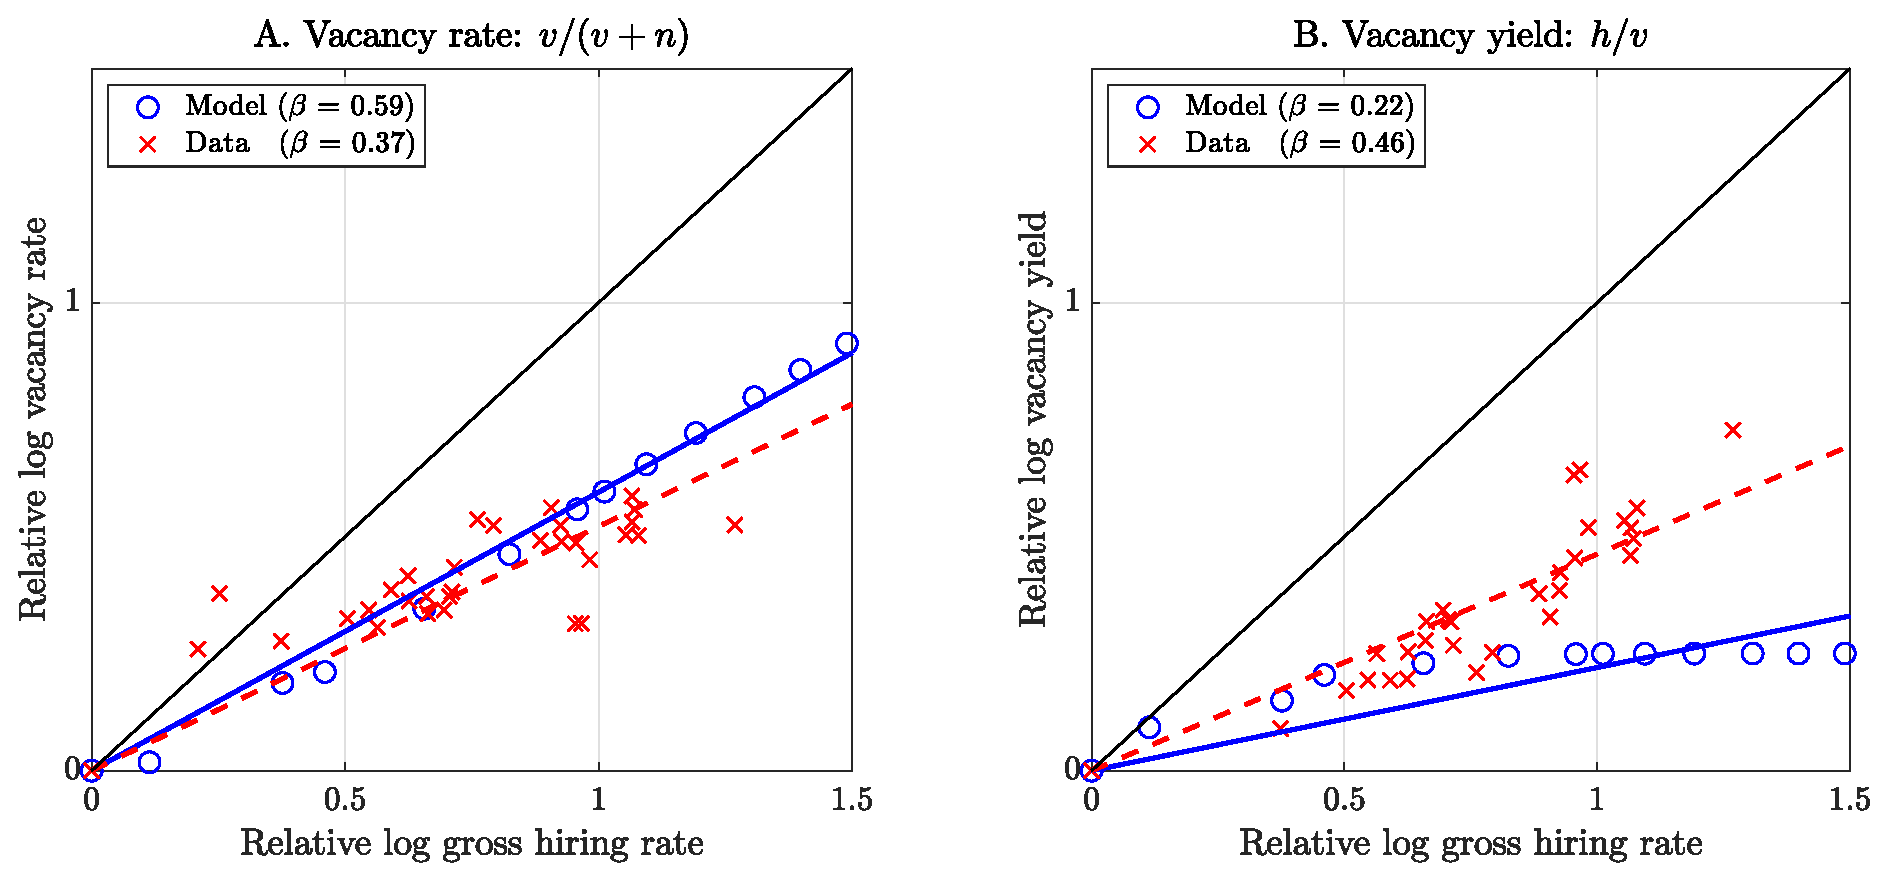
\includegraphics[width=15cm]{\MATLABfigureDir/Fig6_VacancyRatesYields_eps}
\caption{Vacancy rates by firm gross hiring rate}\label{figure:_VacDec}\vspace*{-0.3cm}
\end{center}
{\footnotesize \underline{Notes}
\textbf{Data}: Establishment-month observations in JOLTS microdata 2002-2018 are pooled in bins,
where bins are determined by net monthly growth rate, and have a width of 1 percent.
Growth rates computed as in \citet{DFH}.
Within bin $b$, total hires $h_b$, total vacancies $v_b$, total employment $n_b$ are computed.
From these, the gross hiring rate $h_b/n_b$, and implied daily vacancy posting rate $vr_b = v_b/(n_b)$ are computed using the daily recruiting model of \citet{DFH}.
\textbf{Model}: The variables are constructed in the same way as in the data.
Points plotted are logs of these variables, differenced about the bin representing a one percent net growth rate.
}
\end{figure}

\paragraph{Internally estimated.}
The remaining parameters are estimated by minimizing the objective function
\vspace*{-.3cm}\begin{equation*}
\mathcal{G}(\bm{\psi})=\Big(\bm{\widehat{m}}-\bm{m(\psi)}\Big)'\mathbf{W}^{-1}
\Big(\bm{\widehat{m}}-\bm{m(\psi)}\Big)
\quad,\quad
\bm{\psi} = \Big\{\mu,\sigma,\alpha,\zeta,A,\xi,\delta,b\Big\}\:,
\vspace*{-.3cm}\end{equation*}
where $\bm{\widehat{m}}$ is a vector of empirical moments and $\bm{m(\psi)}$ are their model counterpart.
The matrix $\mathbf{W}$ contains squares of the data moments on the main diagonal and zeros elsewhere.\footnote{
    Our moments are taken from various data sources and in most instances we cannot compute variances of the moments, let alone covariances with other moments.}
We target eight moments that are relatively standard to firm dynamics and frictional labor market literatures.
While this remaining subset of parameters is jointly estimated, some moments are particularly informative about some parameters. Next, we briefly outline our logic.

The drift of productivity, $\mu$, is informed by the (unweighted) firm exit rate.
The more negative the drift, the faster firms exit.
The standard deviation of productivity shocks, $\sigma$, is informed by the standard deviation of annual log employment growth.
If shocks are larger, employment is more volatile.
Decreasing returns, $\alpha$, is informed by the employment share of firms with more than 500 employees.
A smaller span of control allows for fewer large firms.
The thickness of the tail of the productivity distribution of entrants, $\zeta$, is informed by job creation among young firms \citep{decker2020}.\footnote{
    A natural alternative would have been to target the productivity gap between entrants (younger than 1 year old) and incumbents. The model does well in this respect. At the estimated parameter vector, this gap is 27 (35) percent in the model (data) \citep{Gavazza2018}.}
Matching efficiency, $A$, is informed by the nonemployment rate, as a more efficient labor market reduces nonemployment.
Relative search efficiency of employed workers, $\xi$, and the exogenous separation rate, $\delta$, are informed by quarterly $EE$ and $EN$ rates.
Finally, the flow value of leisure, $b$, is informed by the job destruction rate of incumbent firms.
The direct effect of $b$ on marginal surplus $S_n(n,z)$ is one-for-one, so under a higher $b$, a productivity shocks is more likely to lead a firm to hit the layoff frontier $S_n(n,z)=0$, and destroy jobs.
Table \ref{table: estimated parameters}C summarizes the parameters estimated by minimum distance.
In Appendix \ref{appx:identification} we discuss identification more formally, and plot the marginal effect of each parameter on its associated target moment and on the objective function.


\subsection{Model fit}\label{sec: nontargeted}
The estimated model is consistent with micro data that was not directly targeted by the estimation.
This data sits at the intersection of firm and worker dynamics:
(i) the distribution of firms and employment, (ii) job and worker flows across the distribution, and (iii) patterns of net poaching across the distribution.


% DISTRIBUTION OF FIRMS AND EMPLOYMENT BY AGE AND SIZE
\begin{figure}[t!]
\begin{center}
\hspace*{-0.5cm}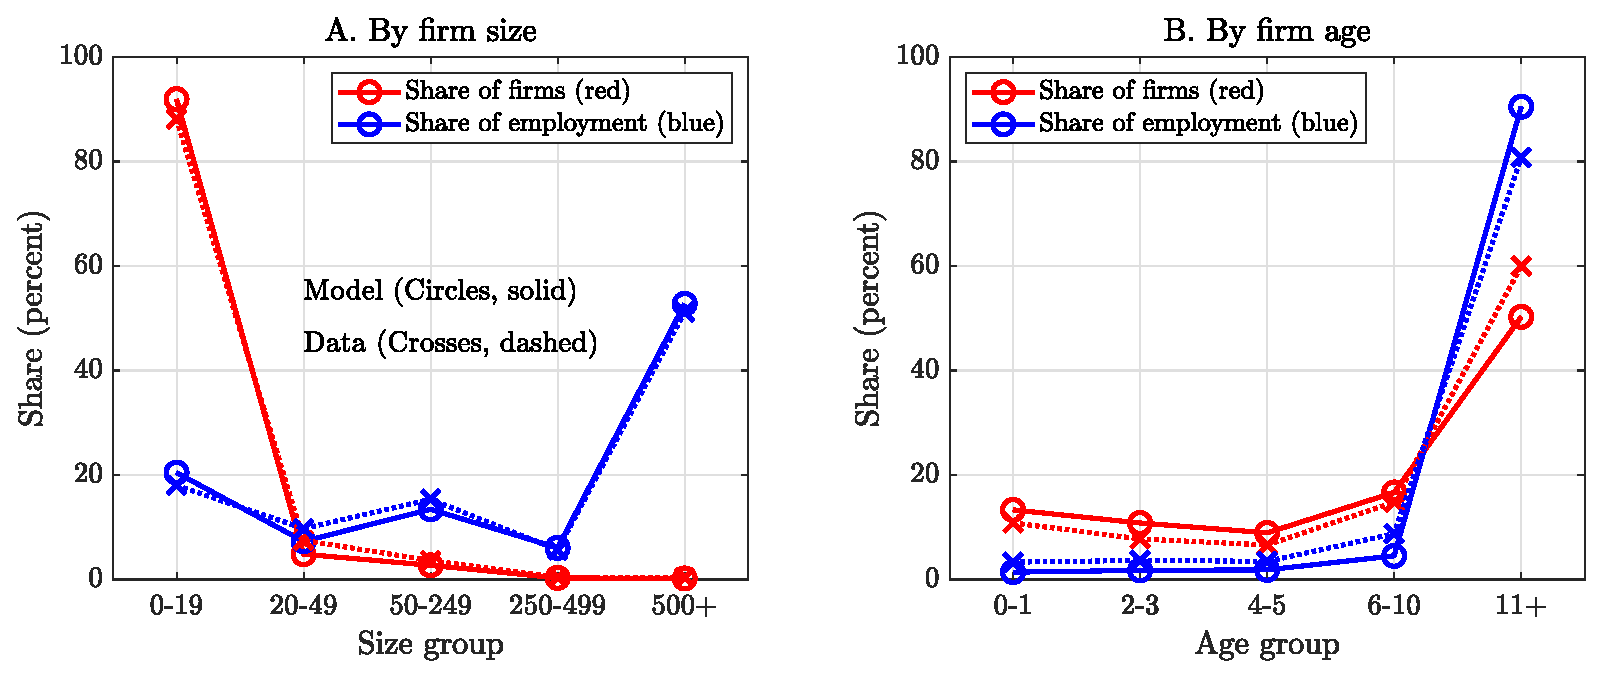
\includegraphics[width=16cm]{\MATLABfigureDir/Fig7_DistributionSizeAge_eps}
\caption{Distribution of firms and employment by firm age and size in data and model}\label{figure:_AgeSize}\vspace*{-.3cm}
\end{center}
{\footnotesize \underline{Source:}
Census BDS
}
\end{figure}
%C:\Users\Simon Mongey\Dropbox\34_Bilal Engbom Mongey Violante\5_Draft\TablesFiguresRevision\Table2Figures.m

\paragraph{1. Distribution of firms and employment.}
Figure \ref{figure:_AgeSize} shows that the model reproduces the skewed firm size and age distributions.
In both data and model, around 90 percent of firms are small (less than 20 employees), but these firms account for only around 20 percent of employment.
Symmetrically, firms with more than 500 employees represent less than 1 percent of firms, but more than 50 percent of employment.
By age, around half of firms are older than 10 years, but these account for 80 percent of employment in the data, and somewhat more in the model.

%%%%%%%%%%%%%%%%%%%%%%%%%%%%%%%%%%%%
% NET POACHING AND MARGINAL SURPLUS
\begin{figure}[t]
\begin{center}
\small{A. Job, worker and firm reallocation by age}\vspace{.2cm}
\hspace*{-0.5cm}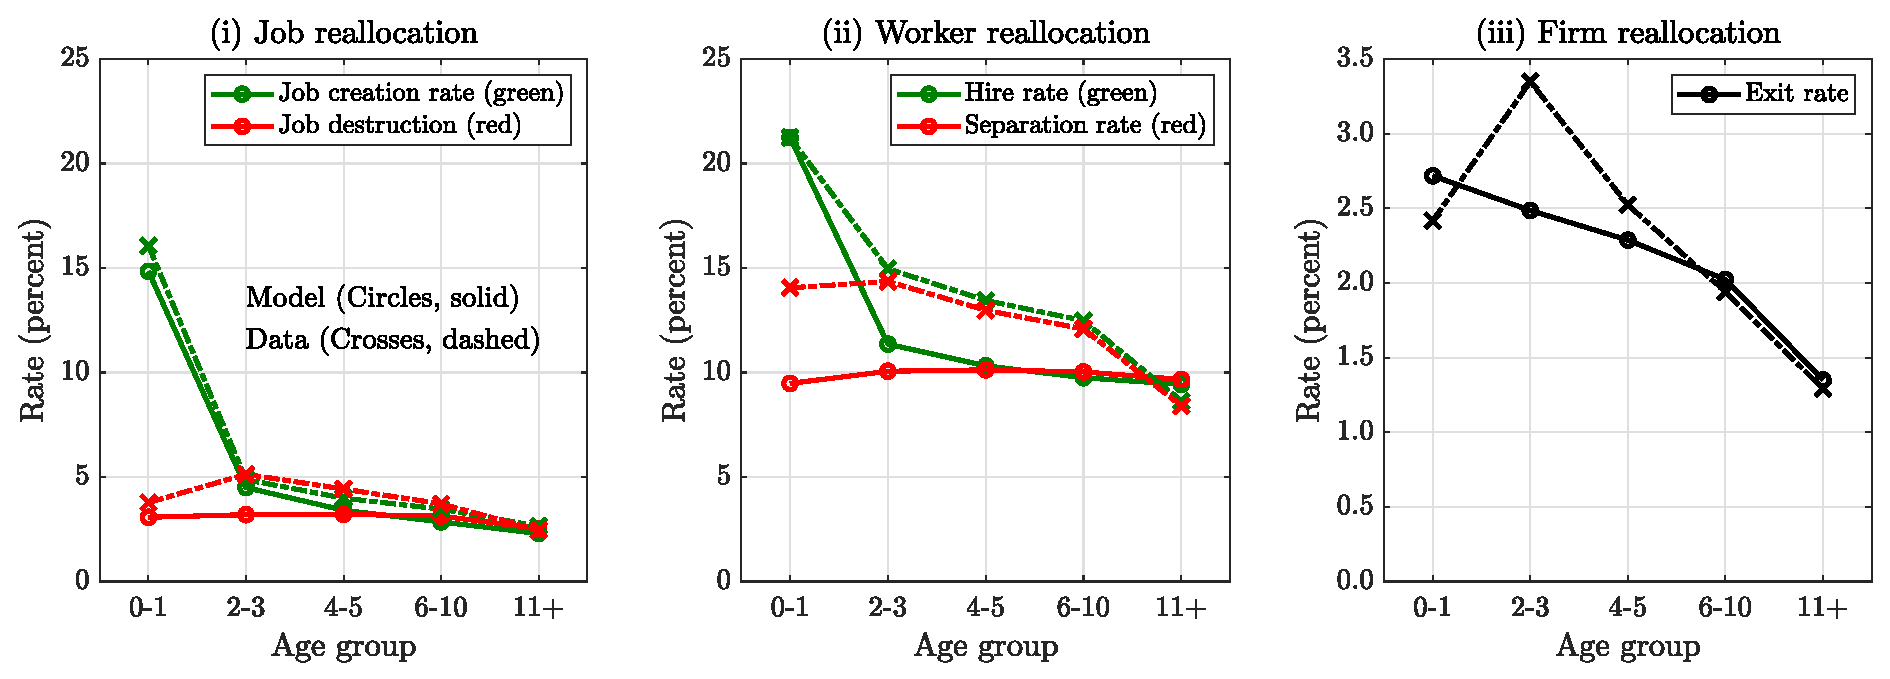
\includegraphics[width=16cm]{\MATLABfigureDir/Fig8A_ReallocationAge_eps}\vspace{.2cm}

\small{B. Job, worker and firm reallocation by size}\vspace{.2cm}
\hspace*{-0.5cm}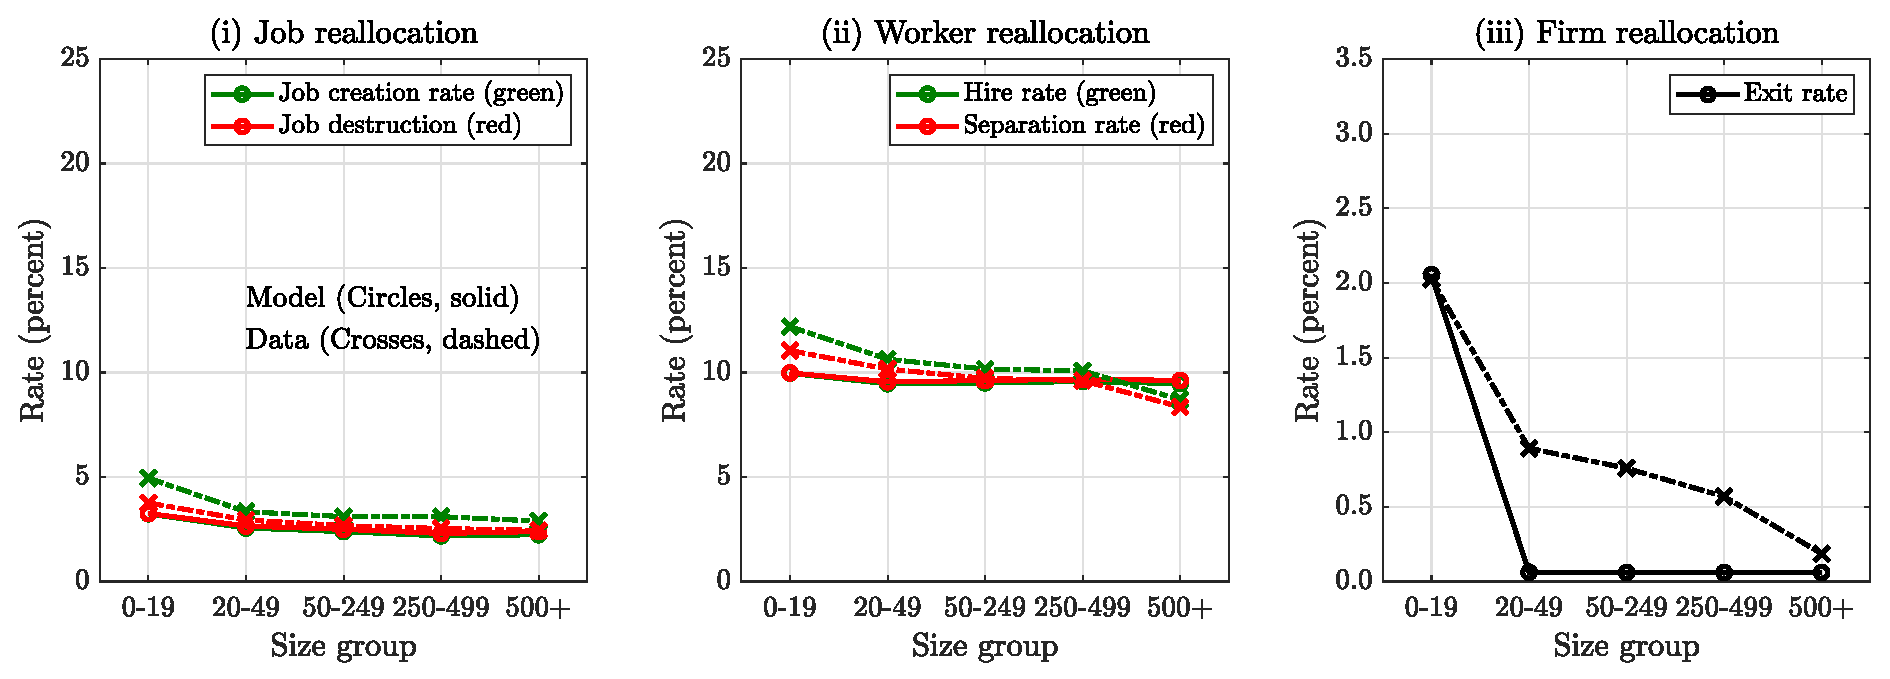
\includegraphics[width=16cm]{\MATLABfigureDir/Fig8B_ReallocationSize_eps}
\caption{Job, worker and firm reallocation by size and age}\label{figure:Reallocation}\vspace*{-0.3cm}
\end{center}
\footnotesize{
\underline{Notes}:
\textbf{Data}:
Census BDS firm data for annual job creation, job destruction and exit.
Quarterly rates constructed by dividing by four.
Census J2J firm data for quarterly hiring and separation rates.
Authors aggregate data into bins given in table which reflect the granularity of J2J data.
Census J2J separations (hires) include separations to (hires from) non-employment.
\textbf{Model}:
Time aggregated to a quarterly frequency.
}
\end{figure}
%C:\Users\Simon Mongey\Dropbox\34_Bilal Engbom Mongey Violante\5_Draft\TablesFiguresRevision\Table3Figures.m
%%%%%%%%%%%%%%%%%%%%%%%%%%%%%%%%%%%%

\paragraph{2. Firm, job and worker reallocation.}
Figure \ref{figure:Reallocation} examines turnover at the level of firms, jobs and workers.
As in the data the rate of job creation peaks for young firms and then declines with age, while job destruction rates are relatively flat.
The model is also consistent with the mild decline in job turnover by size.
Not shown in the figure, in the data (model) 16 percent (15 percent) of all jobs are created by new firm births and 28 percent (26 percent) by firms less than 10 years old.
In terms of worker flows,  EE transitions allow the model to account for the key fact that worker reallocation rates are around three times as large as job reallocation rates, thus generating the right amount of churning.
In the cross-section, the model can reproduce the stark negative empirical relationship between hiring rates and firm age, but struggles to match the gradient at which the separation rate declines with age in the data after age 3.
The model is also in line with the mild decline in worker turnover by size.
The model reproduces the negative gradient for firm exit with respect to age observed in the data.
Absent jumps in the productivity process, firms slowly shrink before exiting, and so every firm  above medium size only exits exogenously: as a result, the model matches small and very large firm exit rates, but not those of intermediate size firms.\footnote{
    Note that the fact that the model slightly overestimates both (i) the hiring and separation rates at old firms (Figure \ref{figure:Reallocation}A), and (ii) the employment share at old firms (Figure \ref{figure:_AgeSize}B), implies that the total share of hires and separations at old firms is larger than in the data (e.g. 15 ppt higher for age 11+ firms).
}

%%%%%%%%%%%%%%%%%%%%%%%%%%%%%%%%%%%%
% NET POACHING AND MARGINAL SURPLUS
\begin{figure}[t]
\begin{center}
\hspace*{-0.5cm}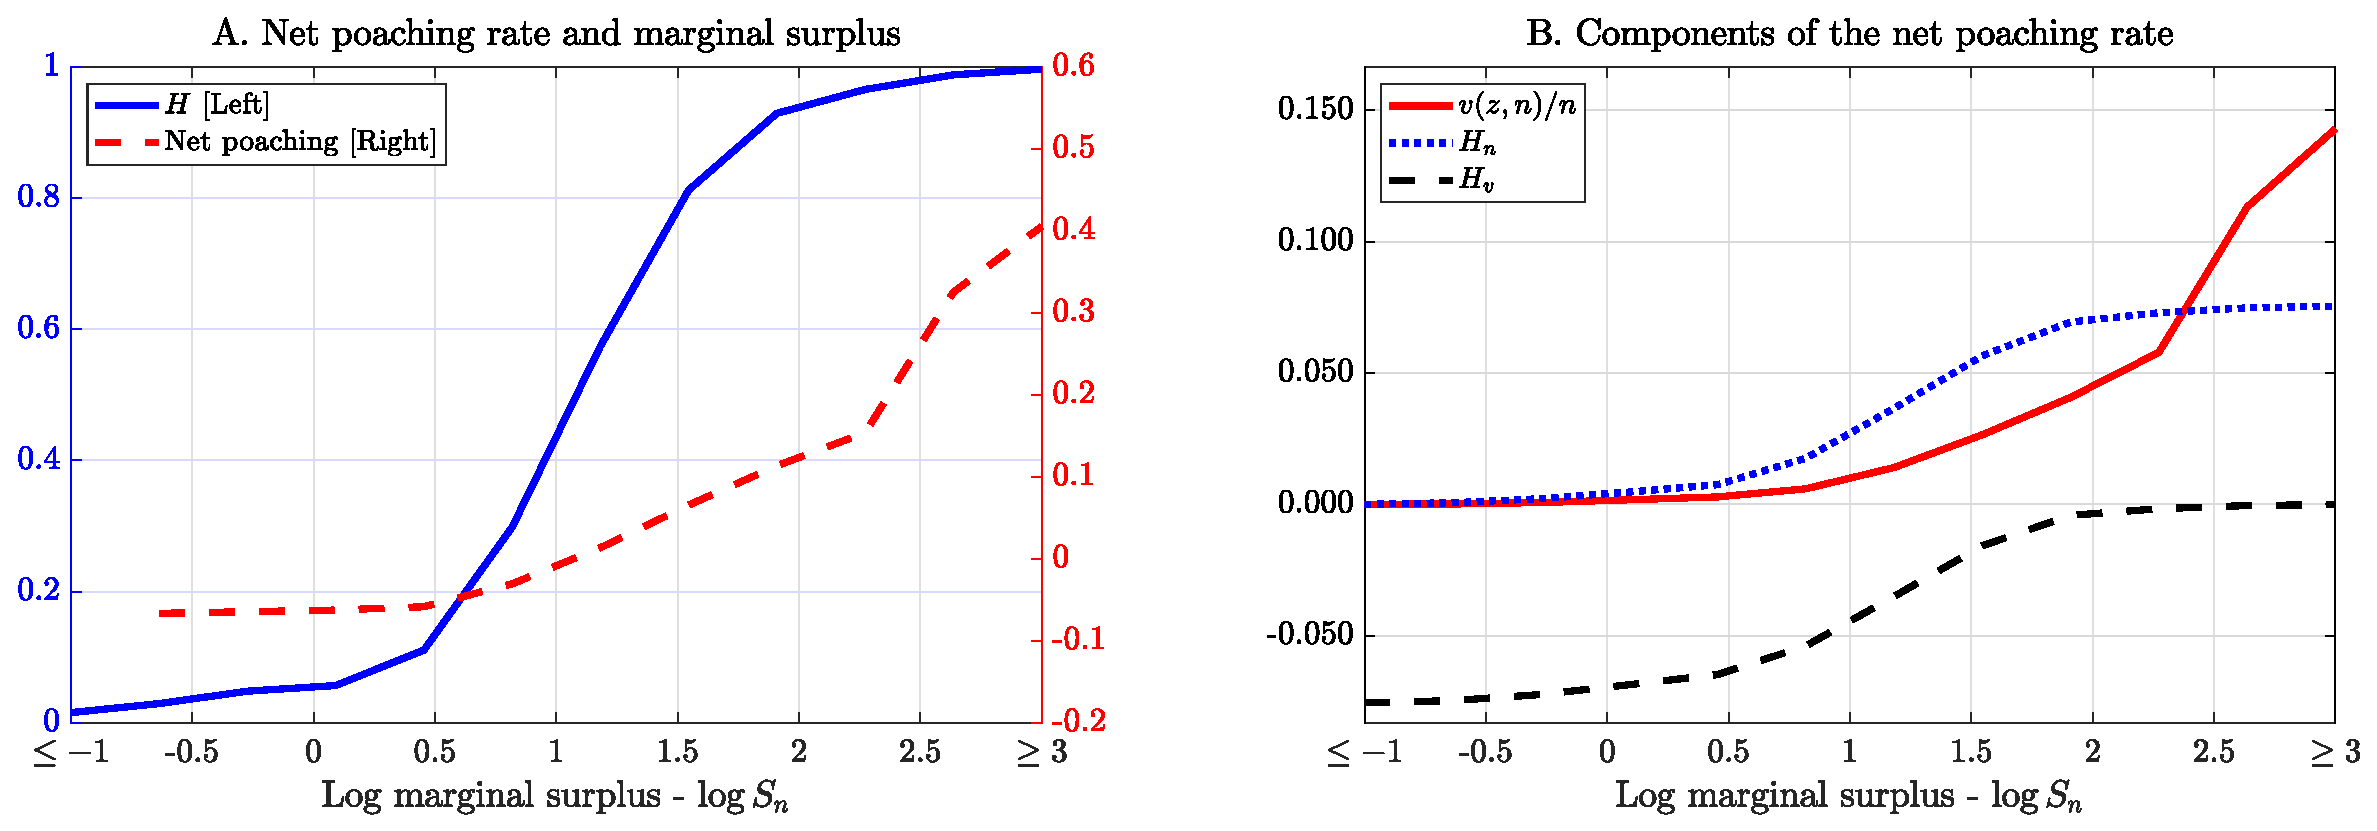
\includegraphics[width=18cm]{\MATLABfigureDir/Fig9_PoachingSurplusDistribution_eps}
\caption{Net poaching and marginal surplus distribution}\label{figure:PoachingSnDecomposition}\vspace*{-0.3cm}
\end{center}
{\footnotesize \underline{Notes:}
\textbf{Panel A.} Net poaching rate $p(S_n)$ by log marginal surplus $S_n$ and the CDF of log marginal surplus.
\textbf{Panel B.} Decomposition of the change in net poaching rate as $S_n$ rises into three components: (i) higher vacancies (red line), (ii) more poaching hires due to higher rank on the job ladder (green line), and (iii) lower poaching separations due to higher rank on the job ladder (blue line).
}
\end{figure}
%C:\Users\Simon Mongey\Dropbox\34_Bilal Engbom Mongey Violante\3_NewCode\NikToSimon\Figure_PoachingSnDecomposition2.m
%%%%%%%%%%%%%%%%%%%%%%%%%%%%%%%%%%%%

\paragraph{3. Net poaching by firm characteristics.}
Figure \ref{figure:PoachingSnDecomposition}A plots the distribution of marginal surplus $H(S_n)$ together with the net poaching rate as a function of marginal surplus.
The CDF reveals that the equilibrium density $h(S_n)$ is quite dispersed.
Net poaching is flat and negative at the low end of the distribution of $S_n$, after which it starts increasing steadily.
What explains this particular shape?
Under our assumptions on vacancy costs, the vacancy rate of the firm $(\widetilde{v}=v/n)$ depends only on marginal surplus.\footnote{
    To see this note that the marginal cost of a vacancy is $c_v(v,n) \propto (v/n)^\gamma$ and, as characterized in Section \ref{sec:comparativestatics}, the marginal benefit of a vacancy depends only on $S_n$.
}
The net poaching rate $p(S_n)$ is therefore:
\vspace*{-.3cm}\begin{equation*}
p(S_n) = \widetilde{v}(S_n)q(\theta)(1-\phi)H_n(S_n) - \lambda^E(\theta)\overline{H}_v(S_n).
\vspace*{-.3cm}\end{equation*}
Higher marginal surplus increases net poaching through three channels:
(i) a higher return to vacancies leads to higher vacancy posting, increasing $EE$ hires $(\uparrow \widetilde{v}(S_n))$;
(ii) conditional on a vacancy, a greater fraction of meetings result in a hire $(\uparrow H_n(S_n))$;
(iii) firm incumbents match with fewer competitors that result in an $EE$ quit $(\downarrow \overline{H}_v(S_n))$.
Figure \ref{figure:PoachingSnDecomposition}B plots these three forces using the following decomposition:
\vspace*{-.2cm}\begin{equation*}
p(S_n) =
\underbrace{\bigg.\int^{S_n}_0\frac{\partial \widetilde{v}(u)}{\partial u}q(\theta)(1-\phi)H_n(u)du}_{\text{Increasing $\uparrow \widetilde{v}(S_n)$}}
+ \underbrace{\bigg.\int^{S_n}_0 \widetilde{v}(u)q(\theta)(1-\phi)h_n(u)du}_{\text{Increasing $\uparrow H_n(S_n)$}}
- \underbrace{\bigg.\lambda^E(\theta)\overline{H}_v(S_n)}_{\text{Decreasing $\downarrow \overline{H}_v(S_n)$}}
\end{equation*}
Firms with very low marginal surplus do not hire and lose all their employees who meet other firms, so net poaching for them approaches $-\lambda^{E}(\theta)$.
In the middle range of $\log{S_n}$ a rise in marginal surplus increases firms' net poaching mostly through changes in its marginal surplus rank which, in turn, expands hires from other firms $(EE^{+})$ and reduces quits $(EE^{-})$.
The vacancy rate initially rises slowly, but as firms get toward the top of the job ladder, vacancies are the only way to keep growing.
This explains why net poaching keeps rising even in the region where the CDF is flattening out, over which poaching translates into negligible jumps up the ladder.

We now project this relationship between net poaching and marginal surplus onto observables in order to compare model and data.
\citet{HHKM2018} document two key empirical patterns: (i) a negligible gradient of net poaching by size, which is inconsistent with wage posting models, and (ii) a steeper negative gradient by age, as young poach from old.
Panels A and B of Figure \ref{figure:J2J2} show that the model matches these patterns quite well, albeit the slope by age is somewhat more pronounced in the model relative to the data.
Size is not a particularly good predictor of where a firm sits on the marginal surplus job ladder.
Consider a vertical slice of Figure \ref{fig:CompStat3}.
At a given size some firms are highly productive, have a high $S_n$, have positive net poaching and create jobs on net.
Meanwhile, other firms are less productive, have a low $S_n$, negative net poaching and destroy jobs on net.
In contrast, young firms are on average small and productive: they sit to the left of $dn=0$ and, having not yet grown, are high on the marginal surplus job ladder.
They therefore display large and positive net poaching rates.\footnote{Put differently, the reason why small firms do not have high net poaching rates on average is because some of them are young and highly productive, but did not have had time to grow yet, while others are small simply because they are unproductive.}

%%%%%%%%%%%%%%%%%%%%%%%%%%%%%%%%%%%%
% NO AGGREGATION ACROSS AGE GROUPS
\begin{figure}[ttt]
\begin{center}
\hspace*{-0.5cm}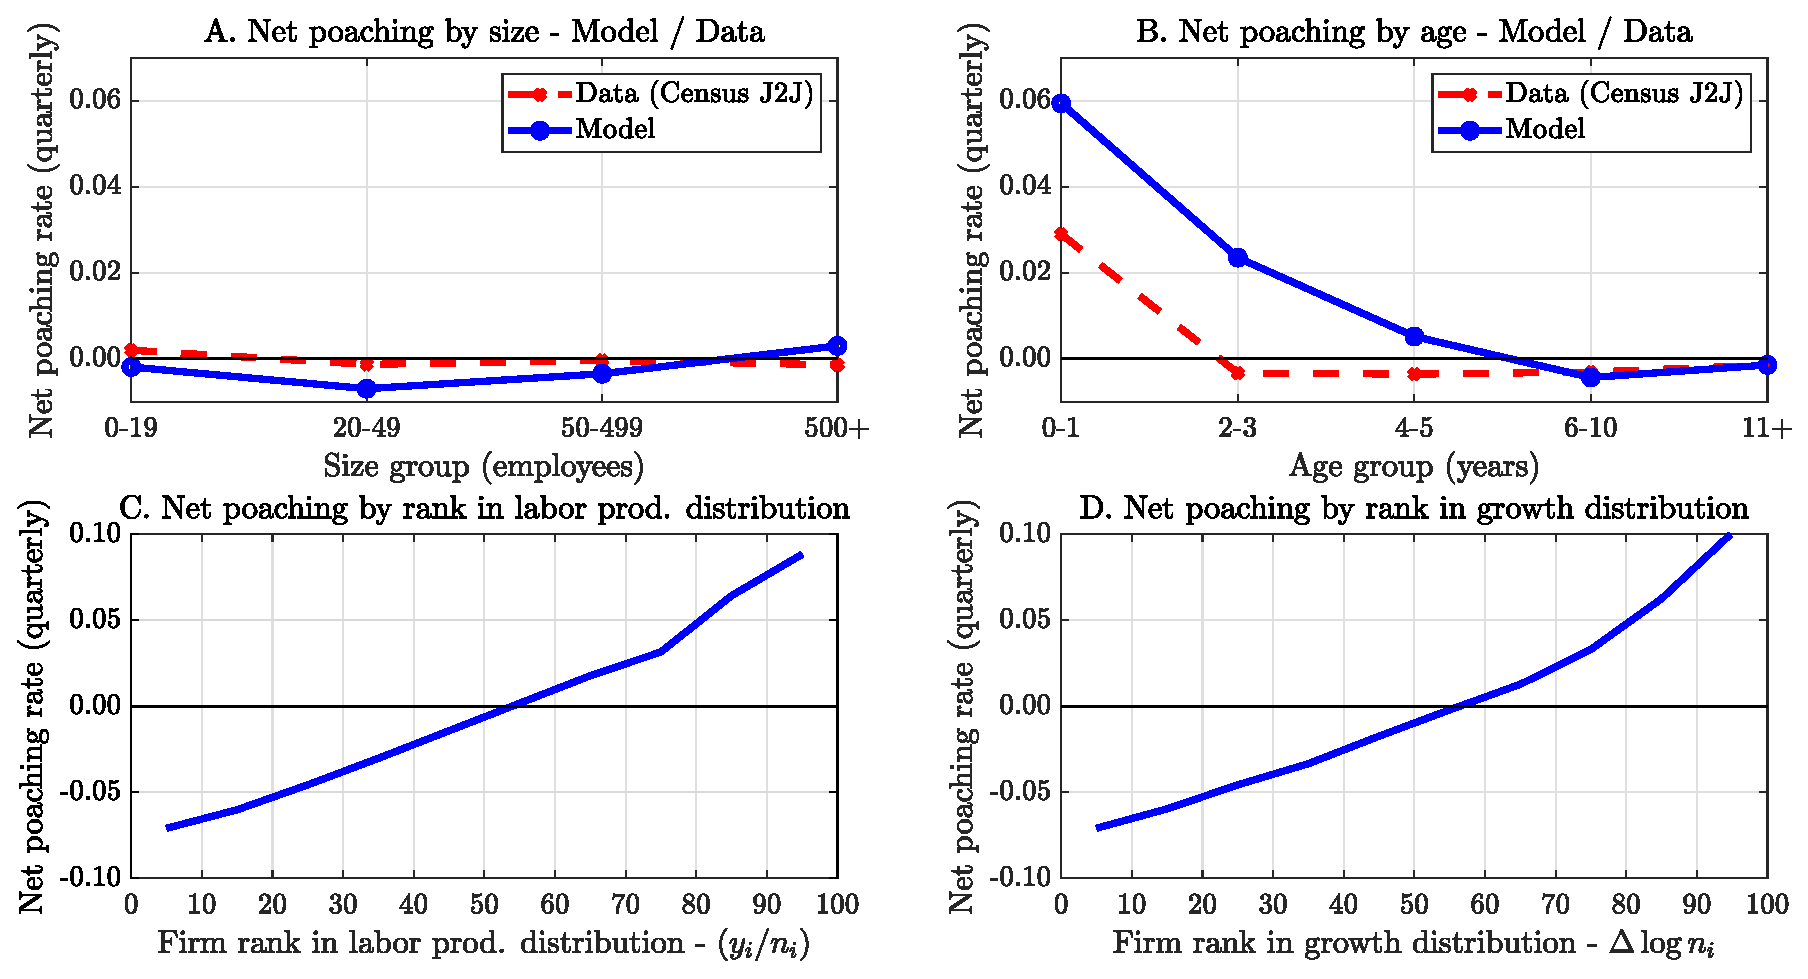
\includegraphics[width=16cm]{\MATLABfigureDir/Fig10_PoachingByCharacteristics_eps}
\caption{Net poaching rates by size, age, labor productivity and net employment growth rate}\label{figure:J2J2}\vspace*{-0.1cm}
\end{center}
\footnotesize{\underline{Notes}:
In panels C and D, firms are ranked according to the employment weighted distribution of labor productivity (C) and employment growth (D).
}
\end{figure}
%%%%%%%%%%%%%%%%%%%%%%%%%%%%%%%%%%%%

Panels C and D of Figure \ref{figure:J2J2} plots net poaching rates as a function of two other, potentially, observable firm characteristics, labor productivity and net employment growth rate.
The model predicts a much higher gradient between these two variables and net poaching rates compared to size and age.
First, marginal surplus is highly correlated with the static marginal product of labor, and the latter is proportional to the average product under our functional form for $y(z,n)$.\footnote{
    One generalization of the model that would weaken this relation is the addition of heterogeneity in the scale of production parameter $\alpha$, as in \citet{Gavazza2018}.
    This would create an additional source of cross-sectional variation in marginal surplus that is orthogonal to $z$. Another one is the addition to the model of forced EE moves (`godfather shocks').}
Second, both in the data and in the model, hires from employment account for much of firm employment growth.
This implies a tight positive relation between net growth rate and net poaching rate.

%%%%%%%%%%%%%%%%%%%%%%%%%%%%%%%%%%%%%%%%%%%%%%%%%%%%%%%%%%%%%%%%%%%%%%%%%%%%%%%%%%%%%%%%%%%%%%%%
\begin{figure}[ttt]
\begin{center}
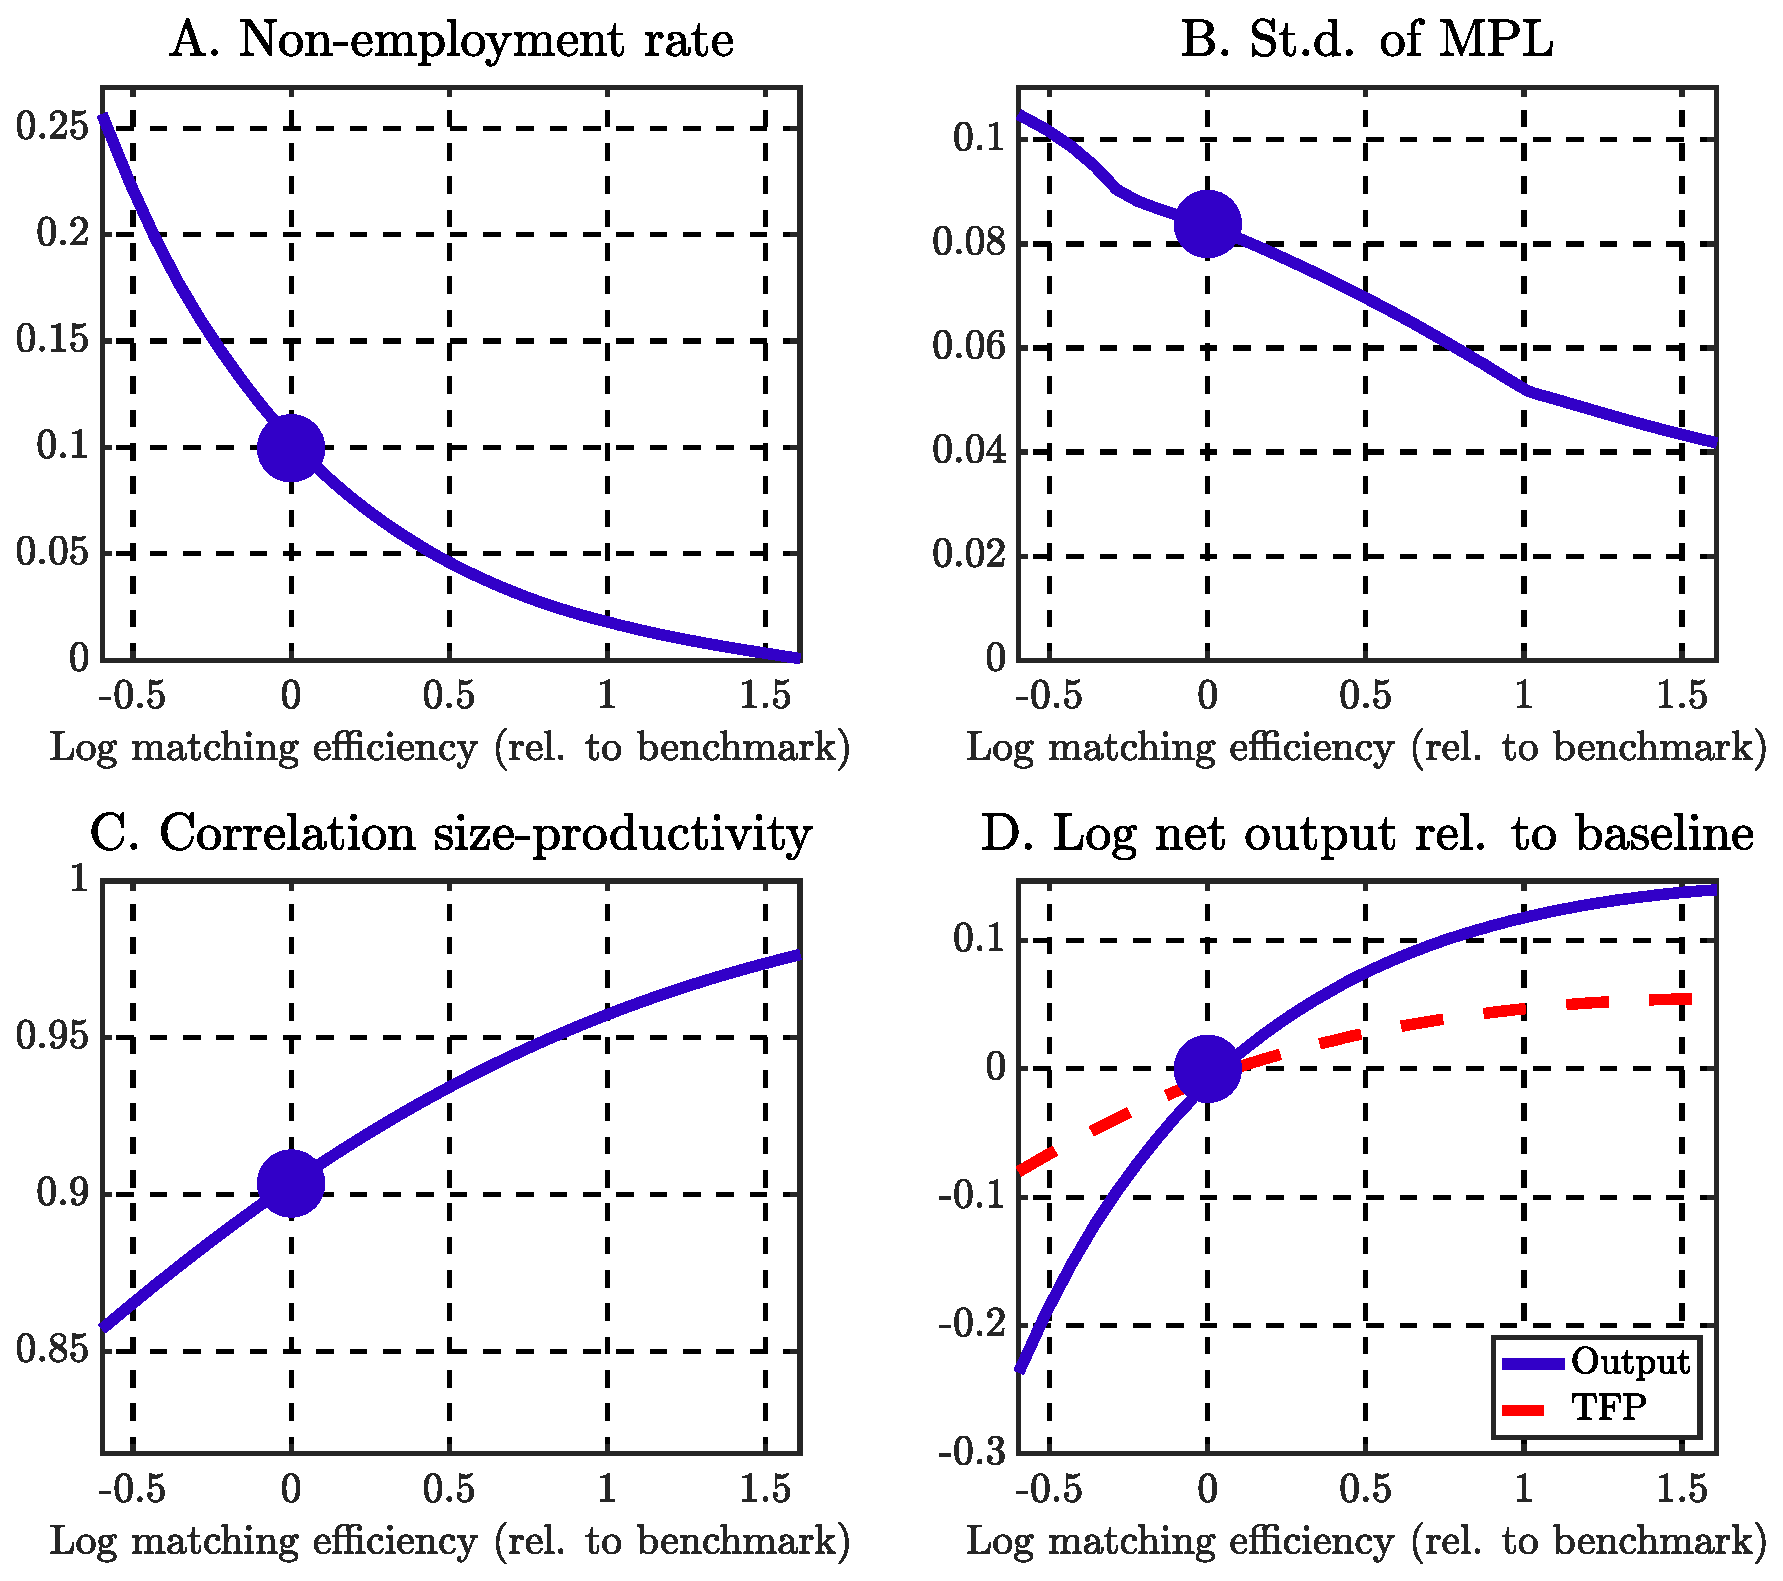
\includegraphics[width=10cm]{\MATLABfigureDir/Fig11_FrictionlessLimit_eps}\vspace*{-.3cm}
%~~~~~~~~~~~~~~~~~~~~~~~~~~~~~~~~~~~~~~~~~~~~~~~~~~~~~~~~~~~~~~~~~~~~~
\caption{Frictionless limit: the effect of increasing match efficiency}\label{figure:Hopenhayn}\vspace*{-.6cm}
\end{center}
\end{figure}
%%%%%%%%%%%%%%%%%%%%%%%%%%%%%%%%%%%%%%%%%%%%%%%%%%%%%%%%%%%%%%%%%%%%%%%%%%%%%%%%%%%%%%%%%%%%%%%%

\section{Search frictions and labor misallocation}\label{sec:misallocation}

It is search and matching frictions, in our model, that impede the instantaneous reallocation of labor across firms. In this section we analyze and quantify the implications of this source of misallocation along three dimensions of the data: cross-section, firm life-cycle and the aggregate business cycle. Because our model is consistent with micro data on both the speed and the direction of the poaching flows across firms that resolve such \textit{frictional misallocation}, it offers a credible platform for these three exercises.

\subsection{Misallocation cost of labor market frictions}
Our model puts us in a unique position to quantify such misallocation by computing the limit as search frictions vanish.
This exercise would not make sense in a model without decreasing returns since it would predict that the most productive firm would hire the entire labor force.
Conversely, we have shown that our economy converges to a competitive equilibrium with a non-degenerate firm size distribution.

Our counterfactual experiment shifts the value of matching efficiency $A$ holding all other parameters fixed at our baseline calibration.
Figure \ref{figure:Hopenhayn} plots model outcomes for a wide range of values for $A$.
As frictions vanish, non-employment falls, the dispersion of marginal products across firms shrinks toward zero, the correlation between size and productivity rises toward one, and aggregate TFP and output grow.\footnote{
    Output is net of vacancy costs. Note that the relationship between frictions and output is concave because the non-employment rate is convex in match efficiency.}

To isolate the role of frictional misallocation, we decompose the change in output into a component due to the allocation of workers across firms, and a component due to higher employment in the economy as a whole, the scale effect.
Imposing an aggregate production function $Y=Z\mathtt{{n}}^\alpha$, then across steady states
\vspace*{-.1cm}\begin{equation*}
\Delta\log{Y} = \Delta\log{Z} + \alpha\Delta\log{\mathtt{{n}}}\quad,\quad Z := \int_{\mathcal{N}\times\mathcal{Z}} z\left(\frac{n}{\mathtt{{n}}}\right)^\alpha\:dH(n,z).
\vspace*{-.1cm}\end{equation*}
The \emph{TFP} term $Z$ captures misallocation and is constant if the distribution of employment across firms is unchanged.\footnote{
    In a constant returns to scale economy, the frictionless limit would be $Z=\max {z}$, since all employment would be at the firm with the highest productivity. Gains from eliminating search frictions would be implausibly large.
}
The misallocation from labor market frictions is sizable in our model.
For example, reducing frictions to an extent that cuts the non-employment rate by half (from 10 to 5 percent) raises aggregate TFP by 3 percent and output by 7 percent. Thus reallocation accounts for nearly half the gains in output. To put this finding in context, the $NE$ rate increases from 0.49 to 0.94 and the $EE$-rate increases from 0.04 to 0.07 (all at quarterly frequency). A five-fold rise in match efficiency relative to the benchmark would virtually eliminate frictional non-employment and boost TFP permanently by 5 percent.

\subsection{Frictional misallocation and the life cycle of superstar firms}
The addition of labor market frictions to a firm dynamics model overcomes a notable shortcoming of competitive environments first identified by \citet{luttmer2011}.
When these models are calibrated to generate the correct cross-sectional variation in firm employment growth rates and the empirical size distribution of firms, they imply that the median age of `superstar' firms ($n>10,000$ workers) is 750 years.
In the data, the median age of such firms is only about 75 years.\footnote{For description of data see \cite{luttmer2011}, Appendix A.
    The data in \cite{luttmer2011} was collected for 2008, on 813 firms with 10,000 or more workers.
    To compute firm age, \cite{luttmer2011} collected data on incorporation taken from a variety of historical sources, for example \textit{Mergent Online}.
}

The root of the problem is that in the data young firms are almost uniformly small and firm employment volatility is not that large.
Viewed through the lens of a frictionless model where size and productivity are perfectly correlated, young firms must be low productivity.
This moment is therefore matched by young firms being way out in the left tail of the productivity distribution.
If shocks are driven by a geometric Brownian motion and chosen to match the empirical volatility of firm growth, then only small shocks are required.
Initially low productivity and small shocks means that it takes a very long time for any firm to get from the left to the very right tail of the productivity distribution.
Since productivity is the only determinant of firm size, then it also takes a very long time for a firm to become a superstar firm.

In our environment, instead, labor market frictions imply that some young firms can be extremely productive but still small as frictions have prevented them from immediately growing large.
Because their initial productivity is already near the upper tail, they remain at the top of the job ladder even after hiring many workers.
This makes expansion cheap, and accommodates rapid growth.
They can therefore move relatively quickly to the tail of the size distribution.
When we simulate firm life cycles in the model, we find that the median age of firms with more than 10,000 workers is 110 years, and hence much closer to the data.
It is thus the existence of frictional labor misallocation---high productivity, but small size firms---that allows the model to be consistent with the cross-sectional size distribution, volatility of firm growth rates, and life-cycle growth trajectories.\footnote{
    Recall that we target the dispersion of firm employment growth in our estimation exercise (Table \ref{table: estimated parameters}).
    The model reproduces quite well the distribution of firms and employment by firm age (Figure \ref{figure:_AgeSize}), and average firm size (Table \ref{table: estimated parameters}).
    Together these imply that we match average size by age and hence average lifecycle growth of firms.
}

%%%%%%%%%%%%%%%%%%%%%%%%%%%%%%%%%%%%
% LUTTMER FIGURE
\begin{figure}[ttt]
\begin{center}
\hspace*{-0.5cm}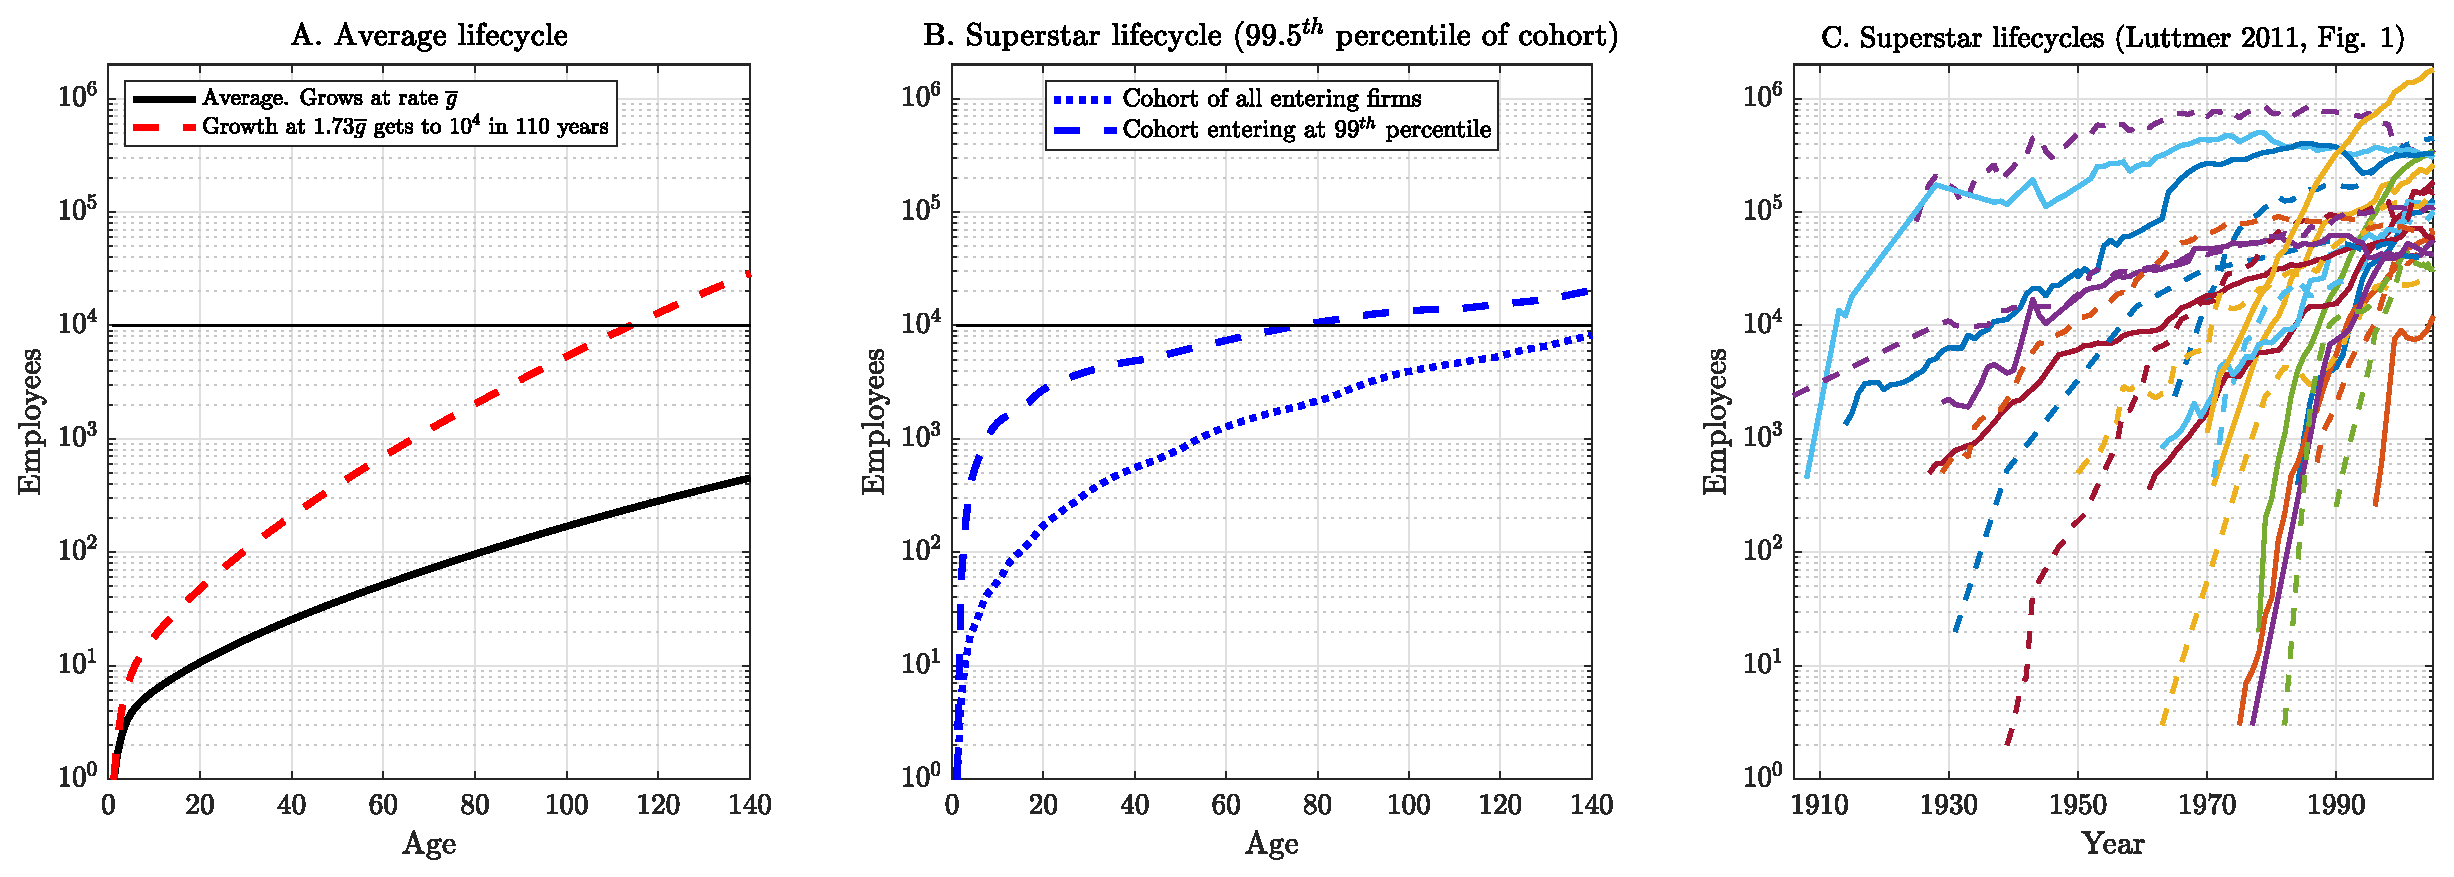
\includegraphics[width=18cm]{\MATLABfigureDir/Fig12_FirmLifecycleSuperstars_eps}
\caption{Comparing the average firm lifecycle to the lifecycle of superstars}\label{figure:Luttmer}\vspace*{-0.1cm}
\end{center}
\footnotesize{\underline{Notes}:
\textbf{Panel A.} plots the average firm size by age, $\overline{n}_a$, (black) which grows at rate $g_a = \overline{n}_{a}/\overline{n}_{a-1}-1$.
The red dashed line plots a counterfactual under which $n_0$ grows at rates $\lambda\times g_a$, where $\lambda=2.05$.
This delivers a firm size of $10,000$ at 110 years, which is the median age of a $10,000$ employee firm in the model.
In \textbf{Panel B.} we take all entering firms (blue dotted), and plot the 99.8$^{th}$ percentile of the firm size distribution at each age.
The blue dashed line takes a mass of firms that enter at the $99^{th}$ percentile of the entrant productivity distribution, and plots the 99.8$^{th}$ percentile of the firm size distribution at each age for this mass of firms.
\textbf{Panel C.} uses the data made publicly available by \cite{luttmer2011} to re-create Figure 1 of that paper.
It plots the employment histories of 25 of the $1,000$ firms that had more than $10,000$ employees in 2008.
% Sentence paraphrased from Luttmer (2011, p 1044).
}
\end{figure}
%%%%%%%%%%%%%%%%%%%%%%%%%%%%%%%%%%%%

Figure \ref{figure:Luttmer} sheds further light on the mechanism behind this finding. Panel A shows than in the model, on average, firms achieve much smaller sizes conditional on surviving for 110 years (black line). One would need a growth rate permanently twice as large in order for the expected firm size at age 110 to exceed 10,000 employees (red line). Instead, from the perspective of the model, being a superstar firm after a century of activity is an extreme tail event both in terms of initial productivity at entry and in terms of sequence of realized productivity shocks along the life cycle (Panel B). Finally, note that the employment trajectory of firms destined to stardom is highly concave both in the data (panel C) and in the model (panel B), and especially so for those firms that already start in the tail (dashed line in panel B).

\subsection{Frictional misallocation in the Great Recession}\label{sec:applications}

The Great Recession provided a raft of new facts regarding the cyclical reallocation of workers across firms.
In particular the two key mechanisms through which labor gets reallocated across productive units are
(i) the entry of new firms which replace unproductive exiting firms and
(ii) the upward movement of workers up the job ladder toward more productive firms.
During the Great Recession both mechanisms slowed considerably.
Firm entry (measured as the number of firms less than 1 year old in the BDS) dropped by almost 30 percent between 2007 and 2009 and has since recovered very slowly. Even allowing for the secular decline in firm entry documented by \citet{pugsley2019grown}, the drop around the Great Recession would be at least 20 percent.\footnote{The entry rate in Figure \ref{figure: j2jdata}A is for establishments for consistency with panel B which is constructed at the city level for which there are no firm-level data. The percentage fall in entry rates of firms and establishments in 2008-2009 is very similar and over the last 40 years the correlation between the two series is 0.98.} The $EE$ rate also fell markedly over the same period (Figure \ref{figure: j2jdata}A).\footnote{
    The exact size of this decline is still debated.
    \citet{HHKM2018} use Census $J2J$ data and report a decline around 30 percent, which Figure \ref{figure: j2jdata} replicates.
    \citet{fujitameasuring2019} argue that Census data overestimate this drop because employment status is only measured quarterly and spurious
poaching transitions (EE from quarter to quarter, but with an `invisible' non-employment spell in between) were much less likely during the
recession, when unemployment spells were quite long.
When they reassess measurement error in CPS data, these authors estimate a drop in the EE rate around 15 percent.}

%%%%%%%%%%%%%%%%%%%%%%%%%%%%%%%%%%%%
% GREAT RECESSION
\begin{figure}[t]
\begin{center}
\hspace*{-0.5cm}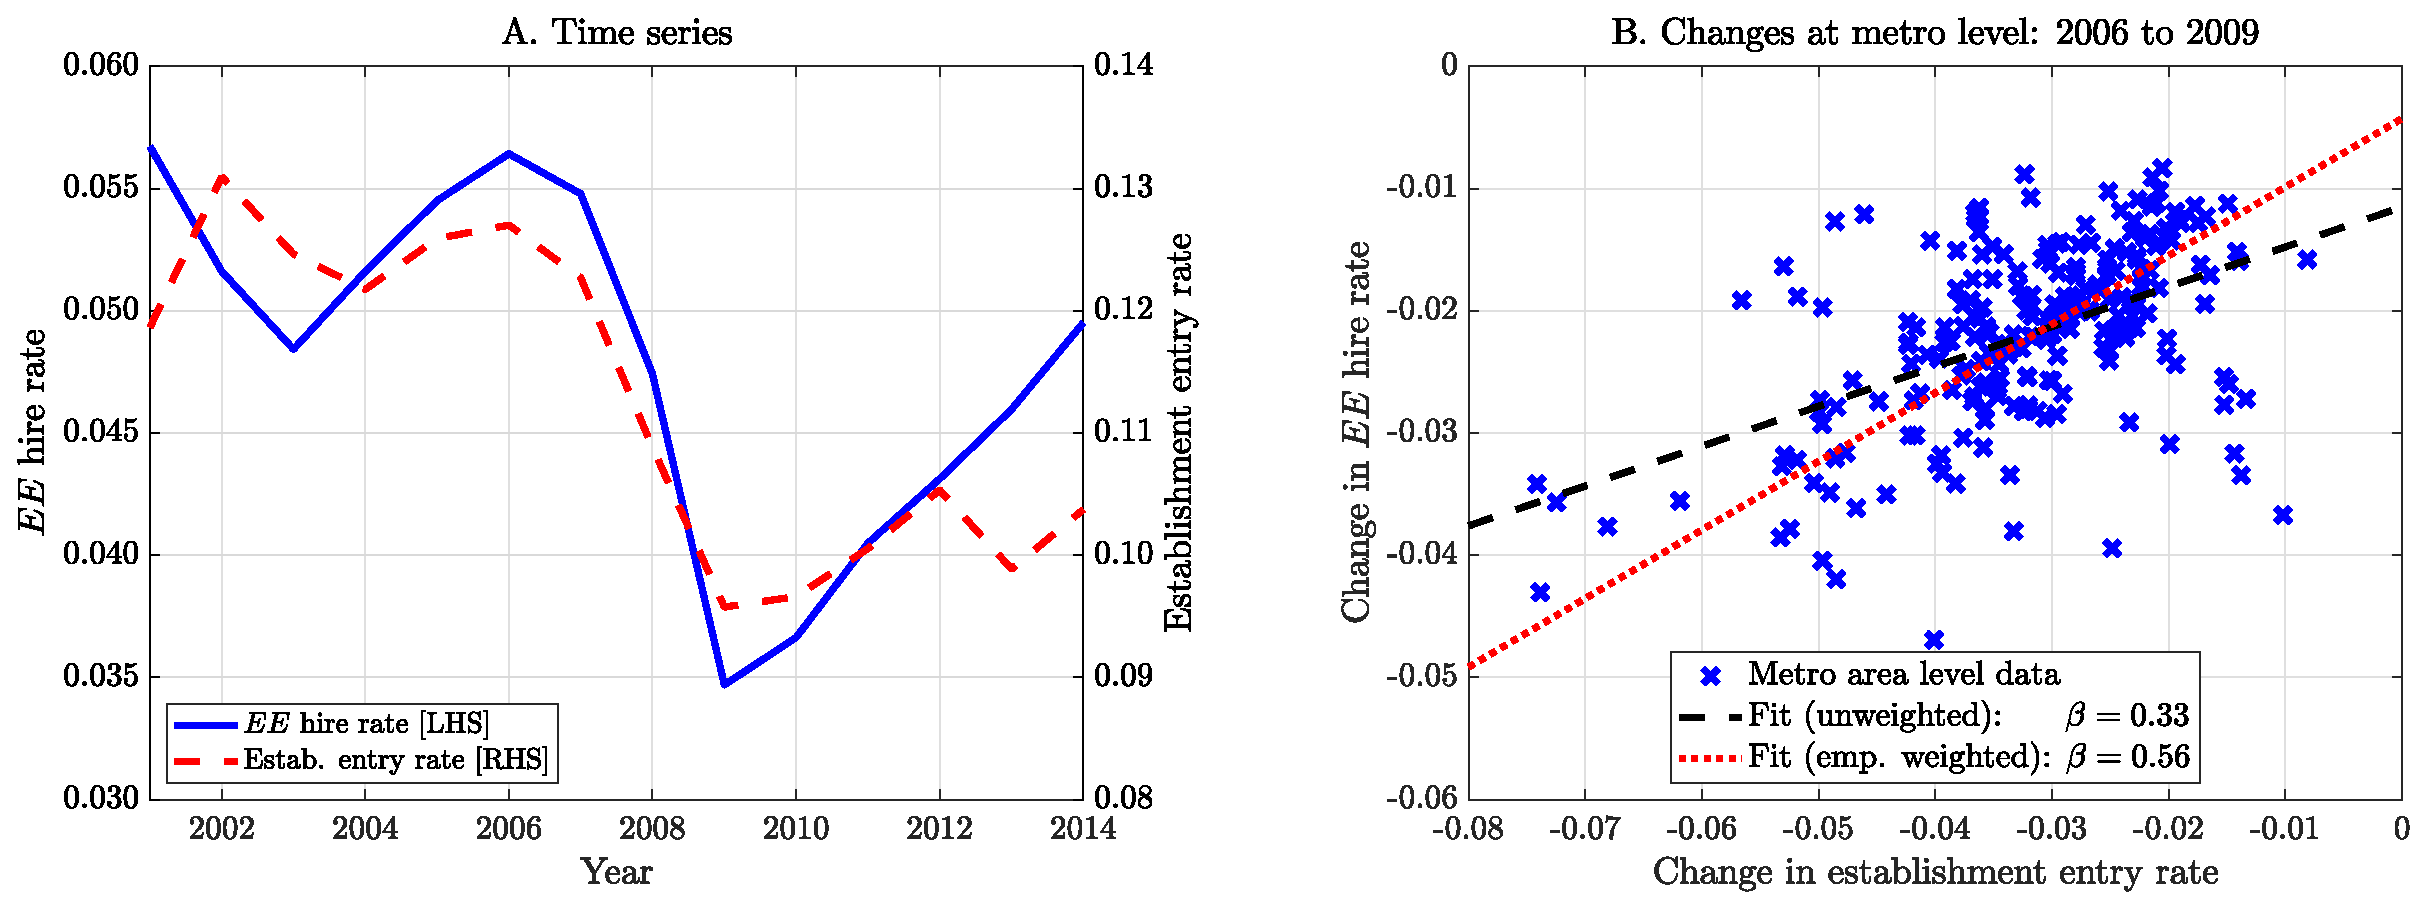
\includegraphics[width=16cm]{\MATLABfigureDir/Fig13_HiringRatesGreatRecession_eps}
\caption{Entry and job-to-job hiring rates over the Great Recession: Aggregate and Cross-section}\label{figure: j2jdata}\vspace*{-0.3cm}
\end{center}
{\footnotesize \underline{Notes:}
Both panels are constructed from the same data at the metro level.
Establishment entry and number of establishments are from the Census BDS data, and used to construct \emph{establishment entry rate}.
Job-to-job hires and employment are from the Census J2J data, and used to construct \emph{$EE$ hire rate}.
The data cover the subset of states that participate in these Census data release programs. These cover more than half of the US population.
}
\end{figure}
%C:\Users\Simon Mongey\Dropbox\Mongey_Park_Williams_HAM\Alex_Firm_Panel\usa\src\plotTS_fmpv_bds_SM.m
%%%%%%%%%%%%%%%%%%%%%%%%%%%%%%%%%%%%

The decline in job-to-job transitions implied a tapering in the process of upgrading from low- to high-rank firms.
\citet{HHKM2018} document a fall in net poaching of high wage firms, those who are presumably at the top of the job ladder.
Similarly, \citet{moscapv} use a structural model to rank firms on the job ladder and estimate that high-rank firms disproportionately curtailed their demand for new labor in the recession.
In short, as they put it: \emph {the job ladder failed, starting from the upper rungs.}

To date, these two facts have not been connected in the literature, since there is a paucity of quantitative structural models that can integrate firm dynamics with on-the-job search.
Theoretically, our environment suggests a natural link between the two, and since our model matches key data on firm and worker dynamics we can also test this link quantitatively.

Theoretically, the mechanism is as follows.
New entrants and young firms account for a sizable share of vacancies and have higher marginal surplus than other firms in the economy.
Following a shock that leads to a drop in the number of entrants, poaching would fall at the top of the ladder which reduces worker reallocation through the middle of the ladder, and so on down to unemployment.

Empirically, this idea is consistent with the correlation observed across cities.
Figure \ref{figure: j2jdata}B combines newly released Census $J2J$ data with Census $BDS$ data at the metro level.
The time-series decline in entry and job-to-job mobility is mirrored in the cross-section of labor markets: cities with larger declines in establishment entry also display larger declines in job-to-job mobility.

We now simulate the Great Recession in our model.
The aggregate shock that best describes the Great Recession is one that worsens financial conditions.
To proxy for a financial shock in our framework, we solve the model under an unexpected temporary increase in the discount rate $\rho$ \citep[as in][]{hall2017high}.
We calibrate the initial jump and the rate of convergence of $\rho$ to match the 5 ppt increase in the unemployment rate and the seven years it took to return to pre-recession levels.\footnote{We calibrate the discount rate shock as follows. We feed in an AR(1) path for $\rho_t$ with a half-life of two years, starting above its steady-state value. To generate a 5 ppt increase in unemployment, the model requires a twenty-fold initial decline in the discount factor. While this value may seem large at first sight, it actually represents a plausible reduction in the stochastic discount factor of firms' shareholders. Indeed, in a `large family' model with curvature in the utility function and consumption equal to output every period, the initial 6\% monthly decline in output that follows from our shock translates into a twenty-fold decline in the stochastic discount factor provided risk aversion is around 10. Values in this range are not uncommon in macro-finance, especially in in the long-run risk \citep{bansal2004risks} and the countercyclical idiosyncratic risk \citep{constantinides2017asset} literatures.}

Because the focus is on short-run dynamics, we replace the long-run free-entry condition with a simple imperfectly elastic entry rule. We posit that every instant, a measure 1 (a normalization) of entrepreneurs contemplate entering. They draw preference shocks for opening a new firm ($\epsilon_1$) and for taking an outside option ($\epsilon_2$) normalized to deliver a payoff of 1. Thus, entrepreneurs solve
\begin{align*}
\max \Big\{ \epsilon_1 \times \frac{\overline{S}_t}{c_0} \ , \ \epsilon_2 \times 1 \Big\}
\end{align*}
where $\overline{S}_t = \int S_t(z,n_0) d\Pi_0(z)$ denotes the expected surplus at firm entry. We assume that $\epsilon_i$ are Frechet distributed with shape parameter $\chi$ and scale normalized to 1. The measure of new firms at $t$ satisfies:
\begin{align*}
M_t = \frac{\bar{S}_t^\chi}{\bar{S}_t^\chi + c_0^\chi}
\end{align*}
We set {$\chi = 0.05$} to match the observed decline in firm entry (-30 percent) following the discount rate shock.

Figure \ref{fig:GRag} describes the response of the model economy to the shock.
The shock lowers the valuation of future revenues at all firms, and as a result, average surplus falls.
Young firms have a disproportionate fraction of their revenues in the future so are especially hard hit, causing entry to collapse (Panel B).
Marginal surplus also falls, which causes an endogenous spike in $EU$ separations (Panel C).
Both lead to a jump in unemployment (Panel A).
Furthermore, declining marginal surplus reduces the return on vacancies \eqref{eq:Rprime}, so aggregate vacancies collapse, job creation contracts, and $UE$ hires decline (Panels D and E).
This leads the jump in unemployment to persist.
With less vacancies and more unemployed workers, the aggregate vacancy yield rises (Panel F).
As in the data, the rise in the vacancy yield is more pronounced for small firms \citep{moscapv}.
For small unproductive firms at the bottom of the ladder, unemployment is the main source of hiring, so as the pool of unemployed job seekers expands, the vacancy filling rate of these firms jumps (Figure \ref{fig:GRag}F).

%%%%%%%%%%%%%%%%%%%%%%%%%%%%%%%%%%%%%%%%%%%%
\begin{figure}[ttt]
\begin{center}
\vspace*{-1cm}
\hspace*{-1cm}
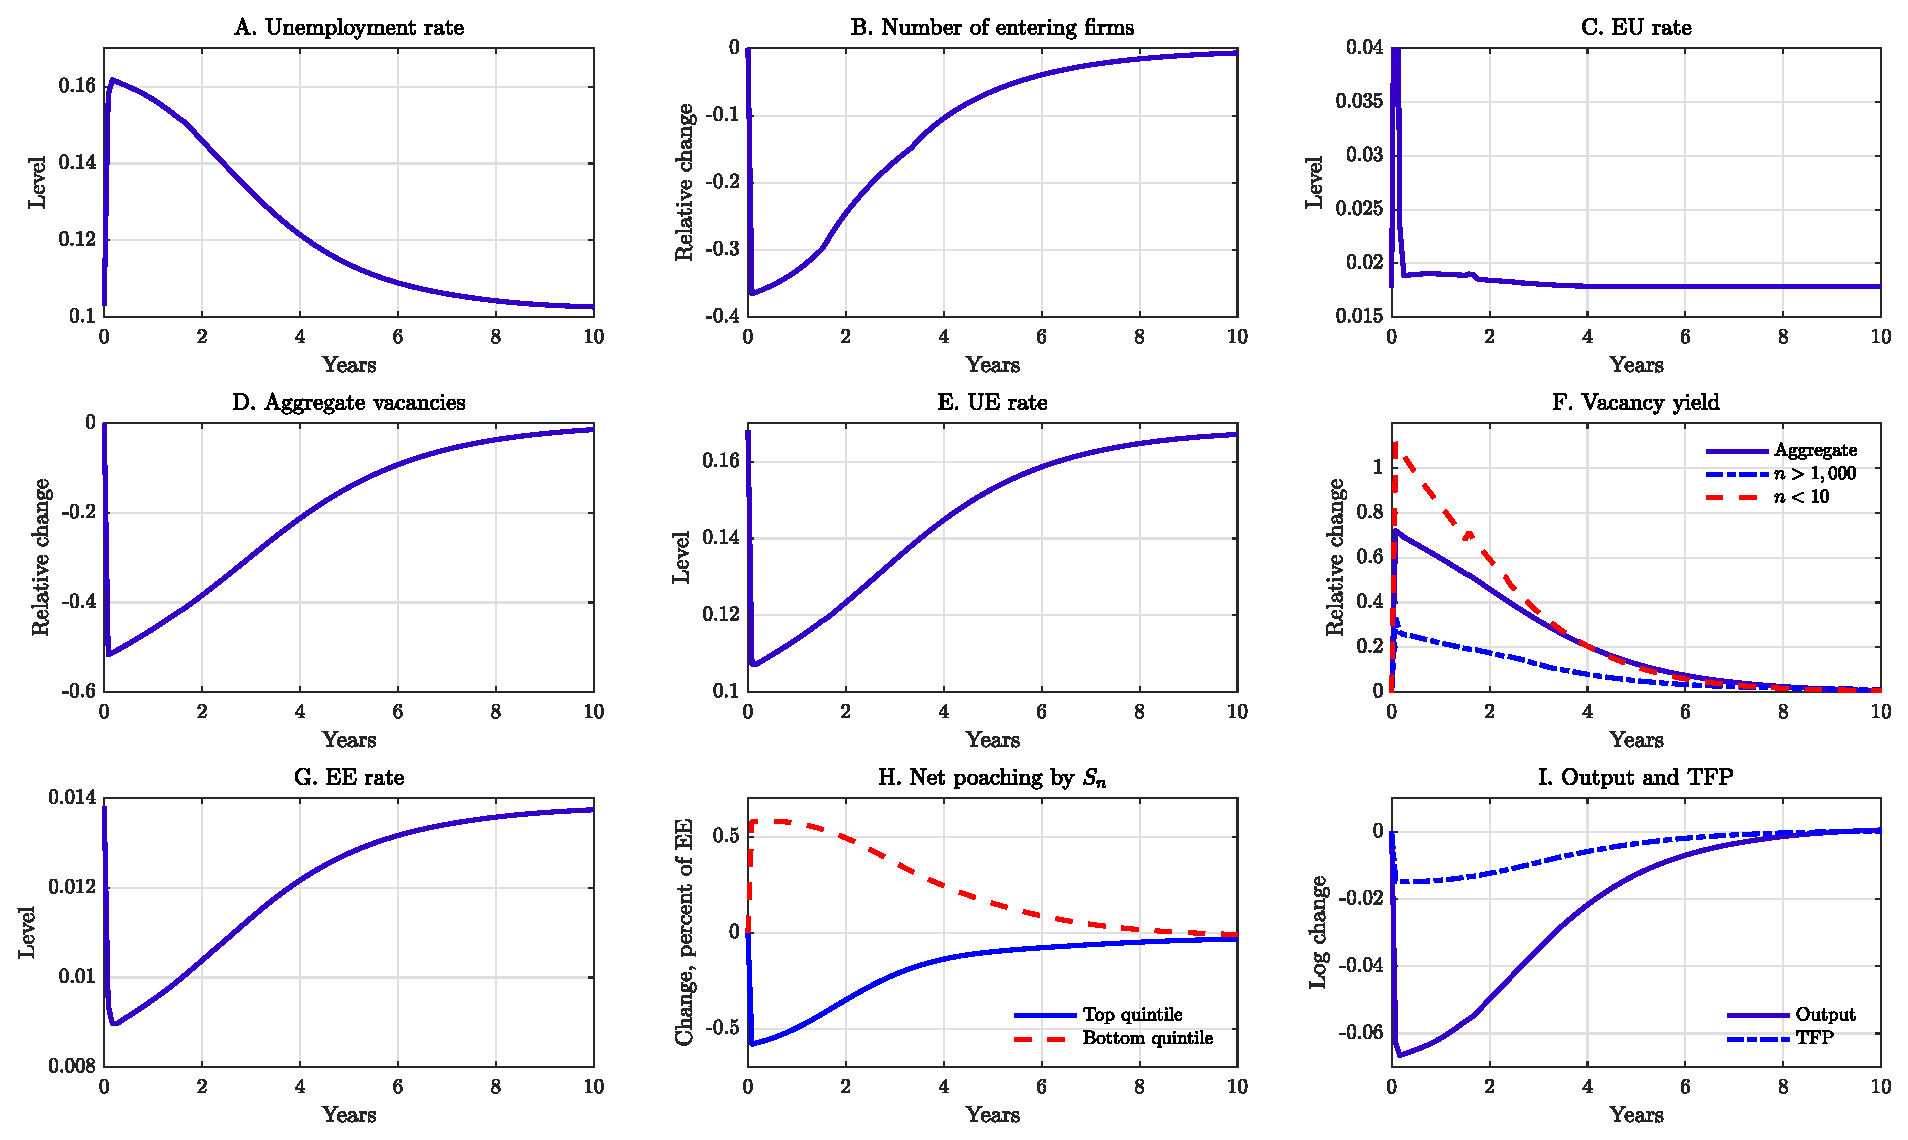
\includegraphics[width=17cm]{\MATLABfigureDir/Fig14_DiscountRateIRF_eps}
\vspace*{-0.5cm}
\caption{Response of the economy following a discount rate shock}\label{fig:GRag}
\vspace*{-.5cm}
\end{center}
\end{figure}
%%%%%%%%%%%%%%%%%%%%%%%%%%%%%%%%%%%%%%%%%%%%


Quantitatively, the experiment matches key non-targeted moments: the $EE$ rate falls about one third (Panel G) and vacancies contract by 50 percent \citep{Gavazza2018}.
The decline in output is 6.5 percent and 9 percent in the data \citep{fernald_NBERannual}.

We now turn to the dynamics of the job ladder.
In the aggregate, the job-to-job mobility rate drops upon impact and slowly recovers (Panel \ref{fig:GRag}G).
In the cross-section, the shift in the vacancy distribution away from high marginal surplus firms---whose poaching rates were most sensitive to their vacancy rates (recall Figure \ref{figure:PoachingSnDecomposition}B)---causes poaching rates to collapse at high marginal surplus firms and, symmetrically, grow at low-marginal surplus firms (Panel H).
This compositional effect reduces the probability that a worker moves from a low- to a high-marginal surplus firm, causing the observed `failure' of the job ladder.

Throughout the recession and its protracted recovery, the slowdown of worker flows towards high-marginal surplus firms exacerbates the misallocation that arises from labor market frictions.
This force grinds down aggregate TFP, and is responsible for about a quarter of the decline in output (Panel I).
The recovery of aggregate productivity is sluggish, with the scars of the recession encoded in the slow moving dynamics of the distribution of employment across firms.

\section{Conclusion}\label{sec:conclusion}
We have set out a new framework to jointly study firm entry and exit, job reallocation, and worker turnover, both through non-employment and through direct job-to-job transitions, in a frictional labor market. The novel feature of the environment, which makes the problem challenging in the presence of random on-the-job search, is diminishing returns to scale in the firm's technology --the hallmark of classic theories of the firm size distribution based on the idea of `span of control'. By extending the contractual environment of \citet{postelvinayrobin2002}, we obtain a tractable `joint value' representation that reduces a potentially unmanageable state space to a very parsimonious one. In contrast with search existing models with linear technology that display a job ladder in exogenous productivity, our model features an endogenous job ladder in \emph{marginal surplus}. Canonical search models and competitive firm dynamics models are special cases of our environment.

We illustrated how to use a calibrated version of the model as a laboratory to shed light on the role of labor misallocation due to search and matching frictions in the cross-section, firm life cycle, and aggregate time series dimension.

Our framework is quite flexible and can be extended in a number of directions while retaining tractability (i.e., a parsimonious state space).
For example, an isomorphic representation of our firm problem is \emph{constant returns to scale} in production of a differentiated final good, which would yield a \emph{decreasing marginal revenue} as under monopolistic competition.
We can therefore easily accommodate imperfect substitutability in the goods market which is a key ingredient of trade models and macroeconomic models with nominal rigidities in goods markets.

The model can also integrate heterogeneity in the scale of production across firms (e.g. to allow for fast-growing `gazelle' firms) and fixed heterogeneity in worker types to address sorting within and across firms.
It is also straightforward to introduce firm-level amenities which have been documented to be important to describe sorting patterns in the data \citep{sorkin2018ranking}.
Once wage determination is incorporated into the model ---a task we left to future work--- shocks to firm-specific or general human capital can also be accommodated to study earnings dynamics within firms and along worker careers.

In all these cases the joint-value representation remains valid and, as long as heterogeneity is discrete and of moderate dimension, the cardinality of the state vector remains manageable.
As is, the model can be used to study the effect of most labor market policies (e.g., unemployment benefits, severance payments, firing taxes and hiring subsidies) on firm dynamics, worker reallocation and aggregate employment and output.

Stationary equilibrium and transitional dynamics can be computed very efficiently and, albeit not in the paper, incorporating aggregate shocks using the approach of \citet{boppart2018exploiting} is straightforward which makes business cycles analysis possible.

In ongoing work \citep{BEMV2021growth}, we show how one can combine this framework with a creative-destruction model of endogenous growth and revisit the nexus between the speed of technical change and aggregate employment \citep{aghion1994growth} in the context of the recent growth slowdown and decline in labor market dynamism. Differently from the canonical models in the endogenous growth literature where optimal size is reached instantaneously, in this hybrid model building to the optimal productive capacity and replacing less productive incumbents is a slow process for an innovator, which requires poaching workers away from other firms. As a result, creative destruction can induce more labor misallocation.

In sum, with the introduction of a well defined notion of firm boundaries (through decreasing returns in technology or downward sloping demand) into a  comprehensive model of frictional labor reallocation across firms, our framework can be potentially useful to study a number of questions in growth, business cycle analysis, labor and trade.

\newpage
%%%%%%%%%%%%%%%%%%%%%%%
%%BIBLIO
%%%%%%%%%%%%%%%%%%%%%%%
\renewcommand{\baselinestretch}{1.04} {\small
\bibliographystyle{econometrica}
\bibliography{MV_bibtex_update}
}

%%%%%%%%%%%%%%%%%%%%%%%%
%%APPENDIX
%%%%%%%%%%%%%%%%%%%%%%%%%
\newpage
\setcounter{page}{1}
\clearpage\newpage
\input{BEMV_ECTA_Appendix.tex}

%%%%%%%%%%%%%%%%%%%%%
\end{document}
%%%%%%%%%%%%%%%%%%%%%

\newpage
\setcounter{page}{1}
\clearpage\newpage
\documentclass[letterpaper,11pt]{article}

\usepackage{amsmath}
\usepackage{etex}
\usepackage{natbib}
\usepackage{amsfonts}
\usepackage{mathpazo}
\usepackage{hyperref}
\usepackage{multimedia}
\usepackage{graphicx, color}
\usepackage{epsfig}
\usepackage{amsthm}
\usepackage{mathtools}
\usepackage{esint}
\usepackage{amssymb}
\usepackage{url}
\usepackage{graphicx}
\usepackage{relsize}
\usepackage{amsfonts}
\usepackage{bm}
\usepackage{fancyheadings}
\usepackage{float}
\usepackage{color}
\usepackage{mathrsfs}
\usepackage{setspace}
\usepackage[mathscr]{euscript}
\usepackage{caption}
\usepackage{subcaption}
\usepackage{pdflscape}
\usepackage{booktabs}
\usepackage[utf8]{inputenc}
\usepackage[T1]{fontenc}
\usepackage{geometry}
\usepackage[dvipsnames]{xcolor}
\usepackage{tikz}
\usepackage{caption}
\usepackage{subcaption}
\usepackage[bottom]{footmisc}
\usepackage{comment}
\usepackage{xr} % to reference external documents

% External documents
\externaldocument{BEMV_Princeton_AB_v13}
\externaldocument{BEMV_Appendix_AB_v13}
\externaldocument{BEMV_WageDetNote_AB_v13}

\setcounter{MaxMatrixCols}{10}

\hypersetup{
    colorlinks,
    linkcolor={red!75!black},
    citecolor={blue!75!black},
}
\pdfminorversion 4
\setlength{\topmargin}{-0.4in}
\setlength{\textheight}{8.85in}
\setlength{\oddsidemargin}{-0.2in}
\setlength{\evensidemargin}{0.0in}
\setlength{\textwidth}{6.93in}
\renewcommand{\baselinestretch}{1.44}%{1.44}
\defcitealias{GMV}{GMV}
\defcitealias{DFH}{DFH}
\setcounter{page}{1}
\usetikzlibrary{decorations.pathreplacing}
\usetikzlibrary{shapes}
\usetikzlibrary{arrows.meta,arrows}
\usetikzlibrary{fit,positioning}
\tikzset{>=latex}
\definecolor{redSM}{RGB}{226,20,61}
\definecolor{greenSM}{RGB}{0,125,0}
\definecolor{blueSM}{RGB}{0,0,178}
\definecolor{hotpinkSM}{RGB}{191,0,127}
\newcommand{\whiteSM}{\textcolor[rgb]{1,1,1}}           % Used for fillers
\newcommand{\alertblue}{\textcolor{blue}}
\newcommand{\alertroyalblue}{\textcolor{RoyalBlue}}
\newcommand{\purple}{\textcolor{purple}}
\newcommand{\hyperlinkblue}{\textcolor{hyperlinkblue}}
\newcommand{\lightblue}{\textcolor{lightblue}}
\newcommand{\alert}{\textcolor{red}}
\newcommand{\tr}{\textcolor{red}}

%\input{tcilatex}

\usepackage{nicefrac}

%~~~~~~~~~~~~~~~~~~~~~~~~~~~~~~~~~~~~~~~~~~~~~~~~~~~~~~~~~~~~~~~~~~~~~~~~~~~~~~~~~~~~
% DIRECTORIES FOR ALL FIGURES AND TABLES IN PAPER
\newcommand{\MATLABfigureDir}{../2_MATLAB_code/Created_figure_files}       % Figures created by MATLAB
\newcommand{\MATLABtableDir}{../2_MATLAB_code/Created_table_files}         % Tables created by MATLAB
\newcommand{\DRAWNfigureDir}{./Figures_without_data}              % Figures drawn 'by hand' and imported as png or tex files (no data or code used)
%~~~~~~~~~~~~~~~~~~~~~~~~~~~~~~~~~~~~~~~~~~~~~~~~~~~~~~~~~~~~~~~~~~~~~~~~~~~~~~~~~~~~








\setlength{\topmargin}{-0.6in}
\setlength{\textheight}{9.05in}
\setlength{\oddsidemargin}{-0.3in}
\setlength{\evensidemargin}{-0.2in}
\setlength{\textwidth}{7.23in}

\begin{document}

\appendix
\begin{center}
\textsc{\huge Appendix II - Not for Publication}\vspace*{.5cm} \\
\textbf{\Large Firm and Worker Dynamics in a Frictional Labor Market}\vspace*{.5cm} \\
\emph{\Large Adrien Bilal, Niklas Engbom, Simon Mongey, Gianluca Violante}\vspace*{.5cm} \\
\end{center}

\small
\setstretch{1.1}

\noindent This Appendix contains the proof of the joint surplus representation in the fully dynamic model, the main result of Section 3 in the main text, and computational details.
Section \ref{appx:dynamicmodel} lays out the notation for the fully dynamic model.
Section \ref{appx:jointvalue_derivation} develops the proof.
Section \ref{appx:computation} contains details on the computation of the stationary equilibrium of the model.

\section{Notation for dynamic model}\label{appx:dynamicmodel}

We first specify the value function of an
individual worker $i$ in a firm with arbitrary state $x$: $V(x,i)$. We then
specify the value function of the firm: $J(x)$. Combining all workers' value
functions with that of the firm we define the joint value: $\Omega(x)$. We
then apply the assumptions from Section 2 which allow us
to reduce $(x)$ to only the number of workers and productivity of the firm, $%
(z,n)$. Finally we take the continuous work force limit to derive a
Hamilton-Jacobi-Bellman (HJB) equation for $\Omega(z,n)$ Applying the
definition of total surplus used above, we obtain a HJB equation in $S(z,n)$
which we use to construct the equilibrium.

\subsection{Worker value function: $V$}

Let $U$ be the value of unemployment. Define separately worker $i$'s value when employed at firm $x$
\emph{before} the quit, layoff and exit decisions, $\bm{V}%
\left(x,i\right) $, and their value \emph{after} these decisions, $V\left(
x,i\right)$.

\paragraph{Value of unemployment.}

Let $h_{U}\left( x\right)$ denote how the state of firm $x$ is updated when
it hires an unemployed worker.\footnote{%
For example, size would be update from $n$ to $n+1$ and possibly some of the
incumbent wages would be bargained down.} Let $\mathcal{A}$ denote the set
of firms making job offers that an unemployed worker would accept. The value of
unemployment $U$ therefore satisfies
\begin{equation*}
\rho U=b+\lambda^U(\theta)\int_{x\in \mathcal{A}}\left[ \bm{V}\left(
h_{U}\left( x\right) ,i\right) -U\right] dH_v\left(x\right)
\end{equation*}%
where $H_v$ is the vacancy-weighted distribution of firms. If $x\notin $ $%
\mathcal{A}$, then the worker remains unemployed.

\paragraph{Stage I.}

To relate the value of the worker pre separation, $\bm{V}(x,i)$, to that
post separation, $V(x,i)$, we require the following notation regarding firm
and co-worker actions. Since workers do not form `unions' within the firm,
all of these actions are taken as given by worker $i$.

\begin{itemize}
\item[-] Let $\epsilon(x)\in \left\{ 0,1\right\}$ denote the exit decision
of firm, and $\mathcal{E=}\left\{ x:\epsilon (x)=1\right\}$ the set of $x$'s
for which the firm exits.

\item[-] Let $\ell(x)\in\{0,1\}^{n(x)}$ be a vector of zeros and ones of length $n(x)$, with generic entry
$\ell_{i}(x)$, that characterizes the
firm's decision to lay off incumbent worker $i\in\{1,\dots,n(x)\}$, and $\mathcal{L=}%
\left\{\left( x,i\right) :\ell _{i}(x)=1\right\}$ the set of $(x,i)$ such
that worker $(x,i)$ is laid off.

\item[-] Let $q^U\left( x\right) \in\{0,1\}^{n(x)}$ be a vector of length $%
n(x)$, with generic entry $q^U_i(x)$ that characterizes an incumbent
workers' decisions to quit, and $\mathcal{Q}^{U}=\left\{ \left(
x,i\right):q^U_i(x)=1\right\} $ the set of $(x,i)$ such that worker $(x,i)$
quits into unemployment.

\item[-] Let $\kappa\left( x\right) =\left( 1-\bm{\ell}\left( x\right)
\right) \circ \left( 1-q_{U}\left( x\right) \right)$ be an element-wise
product vector that identifies workers that are kept in the firm, and $%
\mathcal{S}=\mathcal{L}\cup\mathcal{Q}^{U}=\left\{\left(x,i\right):%
\kappa_{i}\left( x\right) =0\right\}$, the set of $(x,i)$ such that worker $%
(x,i)$ separates into unemployment.

\item[-] Let $s(x,\kappa(x))$ denote how the state of firm $x$ is updated
when workers identified by $\kappa(x)$ are kept. This includes any renegotiation.
\end{itemize}

\noindent Given these sets and functions, the pre separation value $\bm{V}\left(
x,i\right) $ satisfies:
\begin{equation*}
\bm{V}\left( x,i\right) =\underbrace{\Big.\epsilon(x)U\Big.}_{\text{Exit}%
} + (1-\epsilon(x))\Big[\underbrace{\Big.\mathbb{I}_{\{(x,i)\notin \mathcal{S}%
\}} V(s(x,\kappa(x)),i)\Big.}_{\text{Continuing employment}} + \underbrace{%
\Big.\mathbb{I}_{\{(x,i)\in \mathcal{S}\}}U\Big.}_{\text{Separations and
Quits}}\Big]
\end{equation*}

\paragraph{Stage II.}

It is helpful to characterize the continuation value of employment post separation
decisions, $V(x,i)$, in terms of the three distinct types of events
described in Figure . First, the value changes due to
\emph{`Direct'} labor markets shocks to worker $i$, $V_{D}(x,i)$. These
include her match being destroyed exogenously or meeting a new potential
employer. Second, the value changes due to labor market shocks hitting
other workers in the firm, $V_{I}(x,i)$, including their matches being
exogenously destroyed or them meeting new potential employers. These events
have an \emph{`Indirect'} impact on worker $i$. Third, the value changes due to
events on the \emph{`Firm'} side, $V_{F}(x,i)$, including the firm
contacting new workers and receiving productivity shocks. Combining
events and exploiting the fact that in continuous time they are mutually
exclusive, we obtain the following, where  $w\left( x,i\right)$ is the wage paid to worker $i$:
\begin{equation*}
\rho V\left( x,i\right) =w\left( x,i\right) +\rho V_{D}\left( x,i\right)
+\rho V_{I}\left( x,i\right) +\rho V_{F}\left( x,i\right).
\end{equation*}

The wage function $w(x,i)$ includes the transfers between worker $i$ and the firm that may occur at the stage of vacancy posting (after separations and before the labor market opens), as discussed in the Appendix Section A in the context of the static example. These transfers can depend on the entire wage distribution inside the firm which is subsumed in the state vector $x$.

\paragraph{Direct events.}

We first characterize changes in value due to labor market shocks directly to worker $i$ in firm $x$, $V_{D}(x,i)$. Exogenous separation shocks arrive at rate $\delta $ and draws of outside offers arrive at rate $\lambda^E(\theta)$ from the vacancy-weighted distribution of firms $H_v$. If worker $i$ receives a sufficiently good outside offer from $x^{\prime }$, she quits to the new firm. We denote by $\mathcal{Q}^{E}(x,i)$ the set of such quit-firms $x^{\prime}$
for $i$. Otherwise, the worker remains with the current firm but with an updated contract. Therefore $V_D(x,i)$ satisfies
\vspace{-0.1in}

{\small
\begin{eqnarray*}
\rho V_{D}\left( x,i\right) = \underbrace{\Bigg.\delta \left[ U-V\left(
x,i\right)\right]}_{\text{Exogenous separation}} &+& \lambda^E(\theta)
\underbrace{\Bigg.\int_{x^{\prime }\in \mathcal{Q}^{E}\left(x,i\right) }%
\left[ \bm{V}\left( h_{E}\left( x,i,x^{\prime }\right),i\right) -V\left(
x,i\right) \right] dH_v\left( x^{\prime }\right)}_{EE \text{ $\mathcal{Q}$uit}}
\\
&+& \lambda^E(\theta) \underbrace{\Bigg.\int_{x^{\prime }\notin \mathcal{Q}%
^{E}\left( x,i\right) }\left[ \bm{V}\left( r\left( x,i,x^{\prime
}\right) ,i\right) -V\left( x,i\right) \right] dH_v\left( x^{\prime }\right)}_{%
\text{Retention}},
\end{eqnarray*}%
}\noindent where $h_{E}\left( x,i,x^{\prime }\right) $ describes how the
state of a poaching firm $x^{\prime}$ gets updated when it hires worker $i$
from firm $x$. Similarly, $r\left( x,i,x^{\prime}\right)$ updates $x$ when---after meeting firm $x^\prime$---worker $i$ in firm $x$ is
retained and renegotiates its value.
In all functions with three arguments $\left( x,i,x^{\prime}\right)$, the
first argument denotes the origin firm, the second identifies the worker,
and the third the potential destination firm.

\paragraph{Indirect events.}

We next characterize changes in value due to the same labor market shocks hitting other workers in firm $x$, $V_{I}(x,i)$. The value $V_{I}(x,i)$ satisfies
\vspace{-0.1in}

{\small
\begin{eqnarray*}
\rho V_{I}\left( x,i\right) = \sum_{j\neq i}^{n\left( x\right)} \Bigg\{
\underbrace{\delta \left[ \bm{\ V}\left( d(x,j),i\right) -V\left(
x,i\right) \right]\Bigg.}_{\text{Exogenous separation}} &+& \lambda^E(\theta)%
\underbrace{\Bigg.\int_{x^{\prime }\in \mathcal{Q}^{E}\left( x,j\right) } %
\left[\bm{V} \left( q_{E}\left( x,j,x^{\prime }\right) ,i\right)
-V\left(x,i\right)\right] dH_v\left( x^{\prime }\right)}_{\text{$EE$ Quit}} \\
&+& \lambda^E(\theta)\underbrace{\Bigg.\int_{x^{\prime }\notin \mathcal{Q}%
^{E}\left( x,j\right) }\left[ \bm{V}\left( r\left( x,j,x^{\prime
}\right) ,i\right) -V\left( x,i\right) \right] dH_v\left( x^{\prime }\right)}_{%
\text{Retention}} \Bigg\},
\end{eqnarray*}%
}where $d(x,j)$ updates $x$ when worker $j$ exogenously separates, and $%
q_{E}\left( x,j,x^{\prime }\right) $ when worker $j$ quits to firm $%
x^{\prime}$.

\paragraph{Firm events.}
Finally, we characterize changes in value due to events that directly impact the firm and hence
indirectly its workers, $V_F(x,i)$.
Taking as given the firm's vacancy posting policy $v(x)$ and
other actions, $V_F(x,i)$ satisfies
\begin{eqnarray*}
\rho V_{F}\left( x,i\right) &=& \\
\text{$UE$ Hire} &&\phi q(\theta)v\left( x\right) \left[ \bm{V}\left(
h_{U}\left( x\right) ,i\right) -V\left( x,i\right) \right] \cdot \mathbb{I}%
_{\left\{ x\in \mathcal{A}\right\} } \\
\text{$UE$ Threat} &&+\phi q(\theta)v\left( x\right) \left[ \bm{V}\left(
t_{U}\left( x\right) ,i\right) -V\left( x,i\right) \right] \cdot \mathbb{I}%
_{\left\{ x\notin \mathcal{A}\right\} } \\
\text{$EE$ Hire} &&+\left( 1-\phi \right)q(\theta)v\left( x\right)
\int_{x\in \mathcal{Q}^{E}\left( x^{\prime },i^{\prime }\right) }\left[
\bm{V}\left( h_{E}\left( x^{\prime },i^{\prime },x\right) ,i\right)
-V\left( x,i\right) \right] dH_n\left( x^{\prime },i^{\prime }\right) \\
\text{$EE$ Threat} &&+\left( 1-\phi \right)q(\theta)v\left( x\right)
\int_{x\notin \mathcal{Q}^{E}\left( x^{\prime},i^{\prime}\right) }\left[
\bm{V}\left( t_{E}\left( x^{\prime },i^{\prime },x\right) ,i\right)
-V\left( x,i\right) \right] dH_n\left( x^{\prime },i^{\prime }\right) \\
\text{Shock} &&+\Gamma _{z}\left[ \bm{V},V\right] \left( x,i\right)
\end{eqnarray*}%
where $t_{U}\left( x\right) $ updates $x$ when an
unemployed worker is met and not hired, but could be possibly used as a
threat in firm $x$. Similarly, $t_{E}(x^{\prime },i^{\prime },x)$ updates
$x$ when worker $i^{\prime }$ employed at firm $x^{\prime }$
is met, not hired, but could be used as a threat. And, with a slight abuse
of notation, $H_n(x^\prime,i^\prime)$ gives the joint distribution of firms $%
x^\prime$ and worker types within firms $i^\prime$.

Finally, $\Gamma _{z}\left[ \bm{V},V\right] \left( x,i\right) $
identifies the contribution of productivity shocks $z$ to the Bellman
equation. At this stage we only require that the productivity process is
Markovian with an infinitesimal generator. Later we will specialize this to
a diffusion process $dz_t = \mu(z_t)dt + \sigma(z_t) dW_t$ such that
\begin{eqnarray}
\Gamma _{z}\left[ \bm{V},V\right] \left( x,i\right) &=&\mu \left( z\right)
\lim_{dz\rightarrow 0}\frac{\bm{V}\left( \left( x,z+dz\right) ,i\right)
-V\left( x,z,i\right) }{dz} \notag \\
&+&\frac{\sigma ^{2}\left( z\right) }{2}%
\lim_{dz\rightarrow 0}\frac{\bm{V}\left( \left( x,z+dz\right) ,i\right) +%
\bm{V}\left( \left( x,z-dz\right) ,i\right) -2V\left( x,z,i\right) }{%
dz^{2}}  \label{eq:D_diffusion}
\end{eqnarray}
In the case that $\bm{V}=V$, this becomes the standard expression for
a diffusion featuring the first and second derivatives of $V$ with respect to $z$: $\Gamma_z[V](x,i) =
\mu(z)V_z(x,z,i) + \frac{1}{2}\sigma(z)^2V_{zz}(x,z,i)$.\footnote{%
Note that in $(\ref{eq:D_diffusion})$ we abuse notation and write the state
as $(x,z)$ with some redundancy since $z$ is clearly a member of $x$. We
also note that we are not constrained to a diffusion process. We could also
consider a Poisson process where, at exogenous rate $\eta$, $z$ jumps
according to the transition density $\Pi(z,z^\prime)$: $\Gamma _{z}\left[
\bm{V},V\right] \left( x,i\right) = \eta[\sum_{z^{\prime }\in Z}\bm{V%
}\left( \left( x,z^{\prime }\right) ,i\right) \Pi \left( z^{\prime
},z\right) -V\left( x,z,i\right)] $.}

In the event productivity changes or $n\left( x\right)$ changes because of
exogenous labor market events, the worker will want to reassess whether to
stay with the firm or not. Additionally, the firm may want to reassess
whether to exit or fire some workers. Bold values $\bm{V}$ capture any
case where the state changes.

\subsection{Firm value function: $J$}

Consistent with the notation we used for workers' values, let $\bm{J}(x)$
and $J(x)$ be the values of the firm at the corresponding points of an interval $dt$.
For now, we take the vacancy creation decision $v\left(
x\right)$ as given. At the end of the section we describe the expected value
of an entrant firm.

\paragraph{Stage I.}
Consistent with the first stage worker value function, we define the firm
value before the exit/layoff/quit decision, where we recall that $\vartheta$ is the firm's value of exit, or scrap value:
\begin{equation*}
\bm{J}\left( x\right) =\epsilon \left( x\right)\vartheta + \left[
1-\epsilon \left( x\right) \right] J\left( s\left( x,\kappa \left( x\right)
\right) \right).
\end{equation*}%

\paragraph{Stage II.}
Given a vacancy policy $v\left( x\right)$, let $J\left( x\right)$ be the
value of a firm with state $x$ \emph{after} the layoff/quit, exit. It is
convenient to split the value of the firm, as we did for the
worker, into three components
\begin{equation*}
\rho J\left( x\right) = \underbrace{\Bigg.y\left( x\right)
-\sum\limits_{i=1}^{n\left( x\right)}w_{i}\left( x,i\right)\Bigg.}_{\text{%
Flow profits}} \quad+\quad \underbrace{\Bigg.\rho J_{W}\left( x\right)\Bigg.}%
_{\text{Workforce events}} +\quad \underbrace{\Bigg.\rho J_{F}\left(
x\right)-c\left( v\left( x\right) ,x\right)\Bigg.}_{\text{Firm events net of
vacancy costs}}.
\end{equation*}%

For a given policy $v(x)$ there is a set of associated transfers between workers and the firm which, as for the worker value function, are implicit in the wage function $w(x,i)$.

The component $J_{W}\left( x\right) $ is given by
\begin{eqnarray*}
\rho J_{W}\left( x\right) &=& \\
\text{Destruction} &&\delta \sum\limits_{i=1}^{n\left( x\right) }\left[
\bm{J}\left( d(x,i)\right) -J\left( x\right) \right] \\
\text{$EE$ Quit} &&+\:\:\lambda^E(\theta)\sum\limits_{i=1}^{n\left( x\right)
}\int_{x^{\prime }\in \mathcal{Q}^{E}\left( x,i\right) }\left[ \bm{J}%
\left( q_{E}\left( x,i,x^{\prime }\right) \right) -J\left( x\right) \right]
dH_v\left( x^{\prime }\right) \\
\text{Retention} &&+\:\:\lambda^E(\theta)\sum\limits_{i=1}^{n\left( x\right)
}\int_{x^{\prime }\notin \mathcal{Q}^{E}\left( x,i\right) }\left[ \bm{J}%
\left( r\left( x,i,x^{\prime }\right) \right) -J\left( x\right) \right]
dH_v\left( x^{\prime }\right).
\end{eqnarray*}%
The component $J_{F}\left( x\right) $ is given by
\begin{eqnarray*}
\rho J_{F}\left( x\right) &=& \\
\text{$UE$ Hire} && \phi q(\theta)v\left( x\right) \left[ \bm{J}\left(
h_{U}\left( x\right) \right) -J\left( x\right) \right] \cdot \mathbb{I}%
_{\left\{ x\in \mathcal{A}\right\} } \\
\text{$UE$ Threat} &&+\:\:\phi q(\theta)v\left( x\right) \left[ \bm{J}%
\left( t_{U}\left( x\right) \right) -J\left( x\right) \right] \cdot \mathbb{I%
}_{\left\{ x\notin \mathcal{A}\right\} } \\
\text{$EE$ Hire} &&+\:\:\left( 1-\phi \right)q(\theta)v\left( x\right)
\int_{x\in \mathcal{Q}^{E}\left( x^{\prime },i^{\prime }\right) }\left[
\bm{J}\left( h_{E}\left( x^{\prime },i^{\prime },x\right) \right)
-J\left( x\right) \right] dH_n\left( x^{\prime },i^{\prime }\right) \\
\text{$EE$ Threat} &&+\:\:\left(1-\phi \right)q(\theta)v\left( x\right)
\int_{x\notin \mathcal{Q}^{E}\left( x^{\prime },i^{\prime }\right) }\left[
\bm{J}\left( t_{E}\left( x^{\prime },i^{\prime },x\right) \right)
-J\left( x\right) \right] dH_n\left( x^{\prime },i^{\prime }\right) \\
\text{Shock} &&+\:\Gamma _{z}\left[ \bm{J},J\right] \left( x\right)
\end{eqnarray*}

Recall that, in continuous time at most one contact is made
per instant. Either one worker is exogenously separated, or one
worker is contacted by another firm, or one worker is met by posting
vacancies (at rate $q(\theta)v(x)$), or a shock hits the firm. We have bold $\bm{J}$'s in each line since after any of these events, the firm may want to layoff some workers or exit, and workers may want to quit.

\paragraph{Entry.}
The expected value of an entrant firm is
\begin{equation}
J_0=-c_{0}+\int \bm{J}\left( x_{0}\right) d\Pi _{0}\left( z_0\right)
\label{eq:D_J0}
\end{equation}%
where $x_{0}$ is the state of the entrant firm which includes only the
random productivity value $z_0$ drawn from $\Pi _{0}$ since we assumed the
initial number of workers is $0$. The argument of the integral is $\bm{J}
$, which incorporates the firm's decision to exit or operate after
observing $z_0$. Entry occurs when $J_0 >0$.


\section{Derivation of the joint value function $\Omega$}
\label{appx:jointvalue_derivation}
We define the \textbf{joint value} of the firm and
its employed workers $\Omega \left( x\right) :=J\left( x\right) +\sum_{i=1}^{n\left(
x\right)}V\left( x,i\right) $. We also define the joint value before exit/quit/layoff
decisions: $\bm{\Omega }\left( x\right) :=\bm{J}\left(
x\right)+\sum_{i=1}^{n\left( x\right) }\bm{V}\left( x,i\right) $.


\subsection{Combinining worker and firm values}

In this section, we show that summing firm and worker
values, then applying these definitions delivers the following Bellman
equation for the joint value:
\begin{eqnarray}
\rho \Omega \left( x\right) &=&y\left( x\right) -c\left( v\left( x\right)
,x\right)  \label{eq:D_omega1} \\
\text{Destruction} &&+\:\:\sum\limits_{i=1}^{n\left( x\right) }\delta \left[
\bm{\Omega }\left( d(x,i)\right) +U-\Omega \left( x\right) \right]
\notag \\
\text{Retention} &&+\:\:\lambda^E(\theta)\sum\limits_{i=1}^{n\left( x\right)
}\int_{x^{\prime }\notin \mathcal{Q}^{E}\left( x,i\right) }\left[ \bm{%
\Omega }\left( r\left( x,i,x^{\prime }\right) \right) -\Omega \left(
x\right) \right] dH_v\left( x^{\prime }\right)  \notag \\
\text{$EE$ Quit} &&+\:\:\lambda^E(\theta)\sum\limits_{i=1}^{n\left( x\right)
}\int_{x^{\prime }\in \mathcal{Q}^{E}\left( x,i\right) }\left[ \bm{%
\Omega }\left( q_{E}\left( x,i,x^{\prime }\right) \right) +\bm{V}\left(
h_{E}\left( x,i,x^{\prime }\right) ,i\right) -\Omega \left( x\right) \right]
dH_v\left( x^{\prime }\right)  \notag \\
\text{$UE$ Hire} &&+\:\:\phi q(\theta)v\left( x\right) \left[ \bm{\Omega
}\left( h_{U}\left( x\right) \right) -U-\Omega \left( x\right) \right] \cdot
\mathbb{I}_{\left\{ x\in \mathcal{A}\right\} }  \notag \\
\text{$UE$ Threat} &&+\:\:\phi q(\theta)v\left( x\right) \left[ \bm{%
\Omega }\left( t_{U}\left( x\right) \right) -\Omega \left( x\right) \right]
\cdot \mathbb{I}_{\left\{ x\notin \mathcal{A}\right\} }  \notag \\
\text{$EE$ Hire} &&+\:\:(1-\phi)q(\theta)v\left( x\right) \int_{x\in
\mathcal{Q}^{E}\left( x^{\prime },i^{\prime }\right) }\left[ \bm{\Omega }%
\left( h_{E}\left( x^{\prime },i^{\prime },x\right) \right) -\bm{V}%
\left( h_{E}\left( x^{\prime },i^{\prime },x\right) ,i^{\prime }\right)
-\Omega \left( x\right) \right] dH_n\left( x^{\prime },i^{\prime }\right)
\notag \\
\text{$EE$ Threat} &&+\:\:(1-\phi)q(\theta)v\left( x\right) \int_{x\notin
\mathcal{Q}^{E}\left( x^{\prime },i^{\prime }\right) }\left[ \bm{\Omega }%
\left( t_{E}\left( x^{\prime },i^{\prime },x\right) \right) -\Omega \left(
x\right) \right] dH_n\left( x^{\prime },i^{\prime }\right)  \notag \\
\text{Shock} &&+\:\:{\Gamma }_{z}\left[ \bm{\Omega },\Omega \right]
\left( x\right) .  \notag
\end{eqnarray}%
This joint value is only written in terms of other joint values
and worker values. However, it involves both firm and worker decisions
through the sets $\mathcal{A}, \mathcal{Q}^{E}$ and the vacancy policy, $v(x)$.

\paragraph{Derivation.}

We start by computing the sum of the workers' values at a particular firm.
Summing values of all the employed workers
\begin{eqnarray*}
\rho \sum\limits_{i=1}^{n\left( x\right) }V\left( x,i\right)
&=&\sum\limits_{i=1}^{n\left( x\right) }w\left( x,i\right) \\
\text{Destructions} &&+\sum\limits_{i=1}^{n\left( x\right) }\delta \left[
U-V\left( x,i\right) \right] \\
\text{Retentions} &&+\lambda ^{E}\sum\limits_{i=1}^{n\left( x\right)
}\int_{x^{\prime }\notin \mathcal{Q}^{E}\left( x,i\right) }\left[ \boldsymbol{V}%
\left( r\left( x,i,x^{\prime }\right) ,i\right) -V\left( x,i\right) \right]
dH_v\left( x^{\prime }\right) \\
\text{$EE$ Quits} &&+\lambda ^{E}\sum\limits_{i=1}^{n\left( x\right)
}\int_{x^{\prime }\in \mathcal{Q}^{E}\left( x,i\right) }\left[ \boldsymbol{V}%
\left( h_{E}\left( x,i,x^{\prime }\right) \right) -V\left( x,i\right) \right]
dH_v\left( x^{\prime }\right) \\
\text{Incumbents} &&+\sum\limits_{i=1}^{n\left( x\right) }\rho V_{I}(x,i) \\
\text{Firm} &&+\sum\limits_{i=1}^{n\left( x\right) }\rho V_{D}(x,i)
\end{eqnarray*}

where the indirect terms due to incumbents and the firm can be written as:
\begin{eqnarray*}
\sum\limits_{i=1}^{n\left( x\right) }\rho V_{I}(x,i) &=& \\
\text{Destructions} &&\sum\limits_{i=1}^{n\left( x\right) }\sum_{j\neq
i}^{n\left( x\right) }\delta \left[ \boldsymbol{V}\left( d(x,j),i\right)
-V\left( x,i\right) \right] \\
\text{Retentions} &&+\sum\limits_{i=1}^{n\left( x\right) }\sum_{j\neq
i}^{n\left( x\right) }\lambda ^{E}\int_{x^{\prime }\notin \mathcal{Q}%
^{E}\left( x,j\right) }\left[ \boldsymbol{V}\left( r\left( x,j,x^{\prime
}\right) ,i\right) -V\left( x,i\right) \right] dH_v\left( x^{\prime }\right) \\
\text{$EE$ Quits} &&+\sum\limits_{i=1}^{n\left( x\right) }\sum_{j\neq
i}^{n\left( x\right) }\lambda ^{E}\int_{x^{\prime }\in \mathcal{Q}^{E}\left(
x,j\right) }\left[ \boldsymbol{V}\left( q_{E}\left( x,j,x^{\prime }\right)
,i\right) -V\left( x,i\right) \right] dH_v\left( x^{\prime }\right) \ , \\
\sum\limits_{i=1}^{n\left( x\right) }\rho V_{F}(x,i) &=& \\
\text{$UE$ Hires} &&qv\left( x\right) \phi \sum\limits_{i=1}^{n\left(
x\right) }\left[ \boldsymbol{V}\left( h_{U}\left( x\right) ,i\right) -V\left(
x,i\right) \right] \cdot \mathbb{I}_{\left\{ x\in \mathcal{A}\right\} } \\
\text{$UE$ Threats} &&+qv\left( x\right) \phi \sum\limits_{i=1}^{n\left(
x\right) }\left[ \boldsymbol{V}\left( t_{U}\left( x\right) ,i\right) -V\left(
x,i\right) \right] \cdot \mathbb{I}_{\left\{ x\notin \mathcal{A}\right\} } \\
\text{$EE$ Hires} &&+qv\left( x\right) \left( 1-\phi \right)
\sum\limits_{i=1}^{n\left( x\right) }\int_{x\in \mathcal{Q}^{E}\left(
x^{\prime },i^{\prime }\right) }\left[ \boldsymbol{V}\left( h_{E}\left(
x^{\prime },i^{\prime },x\right) ,i\right) -V\left( x,i\right) \right]
dH_n\left( x^{\prime },i^{\prime }\right) \\
\text{$EE$ Threats} &&+qv\left( x\right) \left( 1-\phi \right)
\sum\limits_{i=1}^{n\left( x\right) }\int_{x\notin \mathcal{Q}^{E}\left(
x^{\prime },i^{\prime }\right) }\left[ \boldsymbol{V}\left( t_{E}\left(
x^{\prime },i^{\prime },x\right) ,i\right) -V\left( x,i\right) \right]
dH_n\left( x^{\prime },i^{\prime }\right) \\
\text{Shocks} &&+\sum\limits_{i=1}^{n\left( x\right) } \Gamma_z[\boldsymbol{V}%
,V](x,i)
\end{eqnarray*}%
We now collect terms.

\paragraph{Destructions.}

When worker $i$ separates from firm $x$, the sum of the changes in values of
all employed workers at its own firm is given by:
\begin{eqnarray*}
\text{Destructions} &=&\delta \left[ U-V\left( x,i\right) \right] +\delta
\sum_{j\neq i}^{n\left( x\right) }\left[ \boldsymbol{V}\left( d(x,i),j\right)
-V\left( x,j\right) \right] =\delta \left[ U+\sum_{j\neq i}^{n\left( x\right) }\boldsymbol{V}\left(
d(x,i),j\right) -\sum_{j=1}^{n\left( x\right) }V\left( x,j\right) \right]
\end{eqnarray*}

\paragraph{Retentions.}

When $i$ renegotiates at firm $x$, the sum of the changes in values of all
employed workers at its own firm is given by:
\begin{eqnarray*}
\hspace*{-1cm}\text{Retentions} &=&\lambda ^{E}\int_{x^{\prime }\notin \mathcal{Q}%
^{E}\left( x,i\right) }\left[ \mathbf{V}\left( r\left( x,i,x^{\prime
}\right) ,i\right) -V\left( x,i\right) \right] dH_v\left( x^{\prime }\right) ++\lambda ^{E}\int_{x^{\prime }\notin \mathcal{Q}^{E}\left( x,i\right)
}\sum_{j\neq i}^{n\left( x\right) }\left[ \mathbf{V}\left( r\left(
x,i,x^{\prime }\right) ,j\right) -V\left( x,j\right) \right] dH_v\left(
x^{\prime }\right) \\
&=&\lambda ^{E}\int_{x^{\prime }\notin \mathcal{Q}^{E}\left( x,i\right) }%
\left[ \mathbf{V}\left( r\left( x,i,x^{\prime }\right) ,i\right)
+\sum_{j\neq i}^{n\left( x\right) }\mathbf{V}\left( r\left( x,i,x^{\prime
}\right) ,j\right) -\sum_{j=1}^{n\left( x\right) }V\left( x,j\right) \right]
dH_v\left( x^{\prime }\right) \\
&=&\lambda ^{E}\int_{x^{\prime }\notin \mathcal{Q}^{E}\left( x,i\right) }%
\left[ \sum_{j=1}^{n\left( x\right) }\mathbf{V}\left( r\left( x,i,x^{\prime
}\right) ,j\right) -\sum_{j=1}^{n\left( x\right) }V\left( x,j\right) \right]
dH_v\left( x^{\prime }\right)
\end{eqnarray*}

\paragraph{Quits.}

Similarly, when $i$ quits firm $x$, the sum of the changes in values of all
employed workers at its own firm is given by:
\begin{equation*}
\text{$EE$ Quits}=\lambda ^{E}\int_{x^{\prime }\in Q\left( x,i\right) }\left[
\boldsymbol{V}\left( h_{E}\left( x,i,x^{\prime }\right) ,i\right) +\sum_{j\neq
i}^{n\left( x\right) }\boldsymbol{V}\left( q_{E}\left( x,i,x^{\prime }\right)
,j\right) -\sum_{j=1}^{n\left( x\right) }V\left( x,j\right) \right] dH_v\left(
x^{\prime }\right)
\end{equation*}

\paragraph{Combining terms.}

Before summing up all these terms, define for convenience the total worker value:
\begin{eqnarray*}
\rho \overline{V}\left( x\right) &=&\sum\limits_{i=1}^{n\left( x\right) }w\left(
x,i\right) \\
\text{Destructions} &&+\sum\limits_{i=1}^{n\left( x\right) }\delta \left[
U+\sum_{j\neq i}^{n\left( x\right) }\boldsymbol{V}\left( d(x,i),j\right)
-\sum_{j=1}^{n\left( x\right) }V\left( x,j\right) \right] \\
\text{Retentions} &&+\lambda ^{E}\sum\limits_{i=1}^{n\left( x\right)
}\int_{x^{\prime }\notin \mathcal{Q}^{E}\left( x,i\right) }\left[
\sum_{j=i}^{n\left( x\right) }\boldsymbol{V}\left( r\left( x,i,x^{\prime
}\right) ,j\right) -\sum_{j=1}^{n\left( x\right) }V\left( x,j\right) \right]
dH_v\left( x^{\prime }\right) \\
\text{$EE$ Quits} &&+\lambda ^{E}\sum\limits_{i=1}^{n\left( x\right)
}\int_{x^{\prime }\in \mathcal{Q}^{E}\left( x,i\right) }\left[ \boldsymbol{V}%
\left( h_{E}\left( x,i,x^{\prime }\right) ,i\right) +\sum_{j\neq i}^{n\left(
x\right) }\boldsymbol{V}\left( q_{E}\left( x,i,x^{\prime }\right) ,j\right)
-\sum_{j=1}^{n\left( x\right) }V\left( x,j\right) \right] dH_v\left( x^{\prime
}\right) \\
\text{$UE$ Hires} &&+qv\left( x\right) \phi \sum\limits_{i=1}^{n\left(
x\right) }\left[ \boldsymbol{V}\left( h_{U}\left( x\right) ,i\right) -V\left(
x,i\right) \right] \cdot \mathbb{I}_{\left\{ x\in \mathcal{A}\right\} } \\
\text{$UE$ Threats} &&+qv\left( x\right) \phi \sum\limits_{i=1}^{n\left(
x\right) }\left[ \boldsymbol{V}\left( t_{U}\left( x\right) ,i\right) -V\left(
x,i\right) \right] \cdot \mathbb{I}_{\left\{ x\notin \mathcal{A}\right\} } \\
\text{$EE$ Hires} &&+qv\left( x\right) \left( 1-\phi \right)
\sum\limits_{i=1}^{n\left( x\right) }\int_{x\in \mathcal{Q}^{E}\left(
x^{\prime },i^{\prime }\right) }\left[ \boldsymbol{V}\left( h_{E}\left(
x^{\prime },i^{\prime },x\right) ,i\right) -V\left( x,i\right) \right]
dH_n\left( x^{\prime },i^{\prime }\right) \\
\text{$EE$ Threats} &&+qv\left( x\right) \left( 1-\phi \right)
\sum\limits_{i=1}^{n\left( x\right) }\int_{x\notin \mathcal{Q}^{E}\left(
x^{\prime },i^{\prime }\right) }\left[ \boldsymbol{V}\left( t_{E}\left(
x^{\prime },i^{\prime },x\right) ,i\right) -V\left( x,i\right) \right]
dH_n\left( x^{\prime },i^{\prime }\right) \\
\text{Shocks} &&+\sum\limits_{i=1}^{n\left( x\right) }\Gamma_z[\boldsymbol{V}%
,V](x,i)
\end{eqnarray*}%
Now sum, up all the previous terms, collect terms and use the definition of $%
\overline{V}\left( x\right) $:
\begin{eqnarray*}
\rho \overline{V}\left( x\right) &=&\sum\limits_{i=1}^{n\left( x\right) }w\left(
x,i\right) \\
\text{Destructions} &&+\sum\limits_{i=1}^{n\left( x\right) }\delta \left[
U+\sum_{j\neq i}^{n\left( x\right) }\boldsymbol{V}\left( d(x,i),j\right) -\overline{V}%
\left( x\right) \right] \\
\text{Retentions} &&+\lambda ^{E}\sum\limits_{i=1}^{n\left( x\right)
}\int_{x^{\prime }\notin \mathcal{Q}^{E}\left( x,i\right) }\left[
\sum_{j=i}^{n\left( x\right) }\boldsymbol{V}\left( r\left( x,i,x^{\prime
}\right) ,j\right) -\overline{V}\left( x\right) \right] dH_v\left( x^{\prime
}\right) \\
\text{$EE$ Quits} &&+\lambda ^{E}\sum\limits_{i=1}^{n\left( x\right)
}\int_{x^{\prime }\in \mathcal{Q}^{E}\left( x,i\right) }\left[ \boldsymbol{V}%
\left( h_{E}\left( x,i,x^{\prime }\right) ,i\right) +\sum_{j\neq i}^{n\left(
x\right) }\boldsymbol{V}\left( q_{E}\left( x,i,x^{\prime }\right) ,j\right) -%
\overline{V}\left( x\right) \right] dH_v\left( x^{\prime }\right) \\
\text{$UE$ Hires} &&+qv\left( x\right) \phi \left[ \sum\limits_{i=1}^{n%
\left( x\right) }\boldsymbol{V}\left( h_{U}\left( x\right) ,i\right) -\overline{V}%
\left( x\right) \right] \cdot \mathbb{I}_{\left\{ x\in \mathcal{A}\right\} }
\\
\text{$UE$ Threats} &&+qv\left( x\right) \phi \left[ \sum\limits_{i=1}^{n%
\left( x\right) }\boldsymbol{V}\left( t_{U}\left( x\right) ,i\right) -\overline{V}%
\left( x\right) \right] \cdot \mathbb{I}_{\left\{ x\notin \mathcal{A}%
\right\} } \\
\text{$EE$ Hires} &&+qv\left( x\right) \left( 1-\phi \right) \int_{x\in
\mathcal{Q}^{E}\left( x^{\prime },i^{\prime }\right) }\left[
\sum\limits_{i=1}^{n\left( x\right) }\boldsymbol{V}\left( h_{E}\left( x^{\prime
},i^{\prime },x\right) ,i\right) -\overline{V}\left( x\right) \right] dH_n\left(
x^{\prime },i^{\prime }\right) \\
\text{$EE$ Threats} &&+qv\left( x\right) \left( 1-\phi \right) \int_{x\notin
\mathcal{Q}^{E}\left( x^{\prime },i^{\prime }\right) }\left[
\sum\limits_{i=1}^{n\left( x\right) }\boldsymbol{V}\left( t_{E}\left( x^{\prime
},i^{\prime },x\right) ,i\right) -\overline{V}\left( x\right) \right] dH_n\left(
x^{\prime },i^{\prime }\right) \\
\text{Shocks} &&+\Gamma_z[\boldsymbol{\overline{V}},\overline{V}](x)
\end{eqnarray*}
Adding this last equation to the Bellman equation for $J(x)$ yields
{\small
\begin{eqnarray*}
\rho \Omega \left( x\right) &=&y\left( x\right) -c\left( v\left( x\right)
,x\right) \\
\text{Destructions} &&+\sum\limits_{i=1}^{n\left( x\right) }\delta \left[
\boldsymbol{J}\left( d(x,i)\right) +U+\sum_{j\neq i}^{n\left( x\right) }\boldsymbol{V%
}\left( d(x,i),j\right) -J\left( x\right) -\overline{V}\left( x\right) \right] \\
\text{Retentions} &&+\lambda ^{E}\sum\limits_{i=1}^{n\left( x\right)
}\int_{x^{\prime }\notin \mathcal{Q}^{E}\left( x,i\right) }\left[ \boldsymbol{J}%
\left( r\left( x,i,x^{\prime }\right) \right) +\sum_{j=i}^{n\left( x\right) }%
\boldsymbol{V}\left( r\left( x,i,x^{\prime }\right) ,j\right) -J\left( x\right) -%
\overline{V}\left( x\right) \right] dH_v\left( x^{\prime }\right) \\
\text{$EE$ Quits} &&+\lambda ^{E}\sum\limits_{i=1}^{n\left( x\right)
}\int_{x^{\prime }\in \mathcal{Q}^{E}\left( x,i\right) }\Bigg[ \boldsymbol{J}%
\left( q_{E}\left( x,i,x^{\prime }\right) \right) +\boldsymbol{V}\left(
h_{E}\left( x,i,x^{\prime }\right) ,i\right) +\sum_{j\neq i}^{n\left(
x\right) }\boldsymbol{V}\left( q_{E}\left( x,i,x^{\prime }\right) ,j\right)
-J\left( x\right) -\overline{V}\left( x\right) \Bigg] dH_v\left( x^{\prime }\right)
\\
\text{$UE$ Hires} &&+qv\left( x\right) \phi \left[ \boldsymbol{J}\left(
h_{U}\left( x\right) \right) +\sum\limits_{i=1}^{n\left( x\right) }\boldsymbol{V}%
\left( h_{U}\left( x\right) ,i\right) -J\left( x\right) -\overline{V}\left(
x\right) \right] \cdot \mathbb{I}_{\left\{ x\in \mathcal{A}\right\} } \\
\text{$UE$ Threats} &&+qv\left( x\right) \phi \left[ \boldsymbol{J}\left(
t_{U}\left( x\right) \right) +\sum\limits_{i=1}^{n\left( x\right) }\boldsymbol{V}%
\left( t_{U}\left( x\right) ,i\right) -J\left( x\right) -\overline{V}\left(
x\right) \right] \cdot \mathbb{I}_{\left\{ x\notin \mathcal{A}\right\} } \\
\text{$EE$ Hires} &&+qv\left( x\right) \left( 1-\phi \right) \int_{x\in
\mathcal{Q}^{E}\left( x^{\prime },i^{\prime }\right) }\left[ \boldsymbol{J}%
\left( h_{E}\left( x^{\prime },i^{\prime },x\right) \right)
+\sum\limits_{i=1}^{n\left( x\right) }\boldsymbol{V}\left( h_{E}\left( x^{\prime
},i^{\prime },x\right) ,i\right) -J\left( x\right) -\overline{V}\left( x\right) %
\right] dH_n\left( x^{\prime },i^{\prime }\right) \\
\text{$EE$ Threats} &&+qv\left( x\right) \left( 1-\phi \right) \int_{x\notin
\mathcal{Q}^{E}\left( x^{\prime },i^{\prime }\right) }\left[ \boldsymbol{J}%
\left( t_{E}\left( x^{\prime },i^{\prime },x\right) \right)
+\sum\limits_{i=1}^{n\left( x\right) }\boldsymbol{V}\left( t_{E}\left( x^{\prime
},i^{\prime },x\right) ,i\right) -J\left( x\right) -\overline{V}\left( x\right) %
\right] dH_n\left( x^{\prime },i^{\prime }\right) \\
\text{Shocks} &&+\Gamma_z[\boldsymbol{J} + \boldsymbol{\overline{V}},J + \overline{V}](x)
-J\left( x\right) -\overline{V}\left( x\right)
\end{eqnarray*}}
Collecting terms and using the definition of $\Omega$ :
{\small
\begin{eqnarray*}
\rho \Omega \left( x\right) &=&y\left( x\right) -c\left( v\left( x\right)
,x\right) \\
\text{Destructions} &&+\sum\limits_{i=1}^{n\left( x\right) }\delta \left[
\boldsymbol{\Omega}\left( d(x,i)\right) +U -\Omega \left( x\right) \right] \\
\text{Retentions} &&+\lambda ^{E}\sum\limits_{i=1}^{n\left( x\right)
}\int_{x^{\prime }\notin \mathcal{Q}^{E}\left( x,i\right) }\left[ \boldsymbol{%
\Omega}\left( r\left( x,i,x^{\prime }\right) \right) -\Omega \left( x\right) %
\right] dH_v\left( x^{\prime }\right) \\
\text{$EE$ Quits} &&+\lambda ^{E}\sum\limits_{i=1}^{n\left( x\right)
}\int_{x^{\prime }\in \mathcal{Q}^{E}\left( x,i\right) }\left[ \boldsymbol{\Omega%
}\left( q_{E}\left( x,i,x^{\prime }\right) \right) +\boldsymbol{V}\left(
h_{E}\left( x,i,x^{\prime }\right) ,i\right) -\Omega \left( x\right) \right]
dH_v\left( x^{\prime }\right) \\
\text{$UE$ Hires} &&+qv\left( x\right) \phi \left[ \boldsymbol{\Omega}\left(
h_{U}\left( x\right) \right) - U -\Omega \left( x\right) \right] \cdot
\mathbb{I}_{\left\{ x\in \mathcal{A}\right\} } \\
\text{$UE$ Threats} &&+qv\left( x\right) \phi \left[ \boldsymbol{\Omega}\left(
t_{U}\left( x\right) \right) -\Omega \left( x\right) \right] \cdot \mathbb{I}%
_{\left\{ x\notin \mathcal{A}\right\} } \\
\text{$EE$ Hires} &&+qv\left( x\right) \left( 1-\phi \right) \int_{x\in
\mathcal{Q}^{E}\left( x^{\prime },i^{\prime }\right) }\left[ \boldsymbol{\Omega}%
\left( h_{E}\left( x^{\prime },i^{\prime },x\right) \right) -\boldsymbol{V}%
\left( h_{E}\left( x^{\prime },i^{\prime },x\right) ,i^{\prime}\right)
-\Omega \left( x\right) \right] dH_n\left( x^{\prime },i^{\prime }\right) \\
\text{$EE$ Threats} &&+qv\left( x\right) \left( 1-\phi \right) \int_{x\notin
\mathcal{Q}^{E}\left( x^{\prime },i^{\prime }\right) }\left[ \boldsymbol{\Omega}%
\left( t_{E}\left( x^{\prime },i^{\prime },x\right) \right) -\Omega \left(
x\right) \right] dH_n\left( x^{\prime },i^{\prime }\right) \\
\text{Shocks} &&+\Gamma_z[\boldsymbol{\overline{\Omega}},\overline{\Omega}](x)
\end{eqnarray*}
}


\subsection{Value sharing}

To make progress on $(\ref{eq:D_omega1})$, we begin by stating seven intermediate results, conditions \textbf{(C-RT)-(C-E)} which we prove from
the assumptions listed in Section 2.2. These results establish how worker values \textbf{$\bm{V}$} in $(\ref{eq:D_omega1})$ evolve in the six cases of hiring, retention, layoff, quits, exit and vacancy creation. Next, we apply conditions \textbf{(C-RT)-(C-E)} to $(\ref{eq:D_omega1})$.

To highlight the structure of the argument, we note a key implication our zero-sum game assumption \textbf{(A-IN)}: during internal negotiation, any value lost to one party must accrue to the other. This feature is obvious in the static model, and extends readily to our dynamic environment. 
In other words, the joint value of the firm plus its incumbent workers is invariant during the negotiation. We use this property extensively in the proof. This generalizes pairwise efficient bargaining---commonly used in one-worker firm models with linear production---to an environment with multi-worker firms and decreasing returns in production.

We now state the seven conditions that we apply to $(\ref{eq:D_omega1})$. In section \ref{sec:proofC} below, we prove how each of them is implied by the
assumptions of Section $2.2$.

\begin{enumerate}
\item[\textbf{(C-RT)}] \textbf{Retentions and Threats.} First, if firm $x$
meets an unemployed worker and the worker is not hired but only used as a
threat, then the joint value of coalition $x$ does not change since threats
only redistribute value within the coalition. Second, when firm $x$ uses employed worker $i^{\prime }$ from firm $x^{\prime }$ as a threat, the joint value of coalition $x$ does not change. Third, when firm $x$ meets worker $i^{\prime }$ at $x^{\prime }$ and the worker is retained by
firm $x^{\prime }$, the joint value of coalition $x^{\prime }$ does not change. Formally,
\begin{equation*}
\bm{\Omega }\left( r\left( x^{\prime },i^{\prime },x\right)
\right)=\Omega (x^{\prime })\quad,\quad \bm{\Omega }\left( t_{U}\left(
x\right) \right) =\Omega (x)\quad,\quad \bm{\Omega }\left( t_{E}\left(
x^{\prime },i^{\prime },x\right) \right)=\Omega (x).
\end{equation*}
Respectively, these imply that the \emph{Retention}, \emph{$UE$
Threat} and \emph{$EE$ Threat} components of $(\ref{eq:D_omega1})$ are equal
to zero.
\item[\textbf{(C-UE)}] \textbf{$UE$ Hires.} An unemployed worker that meets
firm $x$ is hired when $x\in\mathcal{A}$. This set consists of firms that
have a joint value after hiring that is higher than the pre-hire joint value
plus the outside value of the hired worker.
Due to the take-leave offer, the new hire receives her outside value, which is the value of unemployment:
\begin{equation*}
\mathcal{A}=\{x|\bm{\Omega}(h_{U}(x))-\Omega(x)\geq U\}
\quad,\quad
\bm{V}\left( h_{U}\left( x\right) ,i\right) =U.
\end{equation*}

\item[\textbf{(C-EE)}] \textbf{$EE$ Hires.} An employed worker $i^{\prime }$
at firm $x^{\prime }$ that meets firm $x$ is hired when $x\in \mathcal{Q}%
^{E}\left(x^{\prime },i^{\prime }\right)$. This set consists of firms that
have a higher marginal joint value than that of the current firm:
\begin{equation*}
\mathcal{Q}^{E}\left( x^{\prime },i^{\prime }\right) =\left\{ x\Big|\bm{%
\Omega }\left( h_{E}\left( x^{\prime },i^{\prime },x\right) \right) -\Omega
\left( x\right) \geq \Omega (x^{\prime })-\bm{\Omega }\left( q_{E}\left(
x^{\prime },i^{\prime },x\right) \right) \right\}.
\end{equation*}
Due to the take-leave offer, the new hire receives her
outside value, which is the
marginal joint value at her current firm:
\begin{equation*}
\bm{V}\left( h_{E}\left( x^{\prime },i^{\prime },x\right) \right)
=\Omega \left( x^{\prime }\right) -\bm{\Omega }\left( q_{E}\left(
x^{\prime },i^{\prime },x\right) \right) .
\end{equation*}

\item[\textbf{(C-EU)}] $EU$\textbf{\ Quits and Layoffs.} An employed worker $%
i$ at firm $x$ quits to unemployment when $\left( x,i\right) \in \mathcal{Q}%
^{U}$. This set consist of states $x$ such that the marginal joint value is
less than the value of unemployment:
\begin{eqnarray*}
\mathcal{Q}^{U}&=&\left\{ (x,i)\Big|\Omega \left( \widehat{s}_{q1}\left(
x,i\right) \right) +U>\Omega \left( \widehat{s}_{q0}\left( x,i\right) \right)
\right\}, \\
%&& \\
\text{where}\quad\quad\widehat{s}_{q1}\left( x,i\right) &=&s\left( x,\left( 1-\left[ q_{U,-i}\left(
x\right) ;q_{U,i}\left( x\right) =1\right] \right) \circ \left( 1-\ell
\left( x\right) \right) \right), \\
\widehat{s}_{q0} \left( x,i\right) &=&s\left( x,\left( 1-\left[ q_{U,-i}\left(
x\right) ;q_{U,i}\left( x\right) =0\right] \right) \circ\left( 1-\ell \left(
x\right) \right)\right).
\end{eqnarray*}%
The first expression captures when worker $i$ quits, and the second where
worker $i$ does not.
Similarly, an $EU$ layoff will be chosen by the firm
when $\left( x,i\right) \in \mathcal{L}$:
\begin{eqnarray*}
\mathcal{L}&=&\left\{ (x,i)\Big|\Omega \left( \widehat{s}_{\ell 1}\left(
x,i\right) \right) +U>\Omega \left( \widehat{s}_{\ell 0}\left( x,i\right)
\right) \right\}, \\
%&& \\
\text{where}\quad\quad\widehat{s}_{\ell 1}\left( x,i\right) &=&s\left( x,\left( 1-\left[ \ell \left(
x\right) ;\ell _{i}\left( x\right) =1\right] \right) \circ \left(
1-q_{U}\left( x\right) \right) \right) , \\
\widehat{s}_{\ell 0}\left( x,i\right) &=&s\left( x,\left( 1-\left[ \ell \left(
x\right) ;\ell _{i}\left( x\right) =0\right] \right) \circ \left(
1-q_{U}\left( x\right) \right) \right) .
\end{eqnarray*}%
The first expression captures when worker $i$ is laid off, and the second
when worker $i$ is not.

\item[\textbf{(C-X)}] \textbf{Exit.} A firm $x$ exits when $x\in \mathcal{E}$%
. This set consists of the states in which the total outside value of the
firm and its workers is larger than the joint value of operation:
\begin{equation*}
\mathcal{E}=\left\{ x\Big|\vartheta +n\left( s\left( x,\kappa \left(
x\right) \right) \right) \cdot U>\Omega \left( s\left( x,\kappa \left(
x\right) \right) \right) \right\} .
\end{equation*}

\item[\textbf{(C-V)}] \textbf{Vacancies.} The expected return to a matched
vacancy $R(x)$ depends only on the joint value, and so the firm's optimal
vacancy policy $v(x)$ depends only on the joint value. The policy $v(x)$
solves
\begin{equation*}
\max_{v}\:\:q(\theta)vR(x)-c\left( v,x\right),
\end{equation*}
where the expected return to a matched vacancy is
\begin{eqnarray*}
R(x) &=& \phi \underbrace{\Big.\left[ \bm{\Omega }\left( h_{U}\left( x\right)
\right) -\Omega \left( x\right) -U\right] \cdot \mathbb{I}_{\left\{ x\in
\mathcal{A}\right\} }}_{\text{Return from unemployed worker match}} \\
&+&\left( 1-\phi \right)\underbrace{\Big.\int_{x\in \mathcal{Q}^{E}\left(
x^{\prime },i^{\prime }\right) }\left\{ \left[ \bm{\Omega }\left(
h_{E}\left( x^{\prime },i^{\prime },x\right) \right) -\Omega \left( x\right) %
\right] -\left[ \Omega \left( x^{\prime }\right) -\bm{\Omega }\left(
q_{E}\left( x^{\prime },i^{\prime },x\right) \right) \right] \right\}
dH_n\left( x^{\prime },i^{\prime }\right)}_{\text{Expected return from
employed worker match}} .
\end{eqnarray*}

\item[\textbf{(C-E)}] \textbf{Entry.} A firm enters if and only if
\begin{equation*}
\int \bm{\Omega }\left( x_{0}\right) d\Pi _{0}(z)\geq c_{0}+n_{0}U.
\end{equation*}
\end{enumerate}

\paragraph{Summarizing (C).}

The substantive result is that all firm and worker decisions and employed
workers' values can be expressed in terms of joint value $\Omega$ and
exogenous worker outside option $U$.

\subsection{Proof of Conditions (C)}

\label{sec:proofC}

\subsubsection{Proof of C-UE and C-RT ($UE$ Hires and $UE$ Threats) \label{ue}}

In this subsection, we consider a meeting between a firm $x$ and an
unemployed worker. Following \textbf{A-IN} and \textbf{A-EN}, the firm internally renegotiates according to a zero-sum game with its incumbent workers and makes a take-leave offer  to the new worker. Intuitively, having the
worker ``at the door'' is identical to having her hired at value $U$ for the
firm and for all incumbent workers: the firm can always make new take-leave
offers to its incumbents after hiring the new worker. Hence, we expect the
firm to make one take-leave offer to the new worker and its incumbents at
the time of the meeting, and not make a new, different offer to is
incumbents afer hiring has taken place.

We start by showing this equivalence formally. To do so, when meeting an
unemployed worker, we let the firm conduct internal renegotiation with its
incumbent workers and make an offer to the new worker. Then, we let a
second round of internal offers take place after the hiring. We introduce
some notation to keep track of values throughout the internal and external
negotiations. To fix ideas, we denote by (IR1) the first round of internal
negotiation, pre-external negotiation. We denote by (IR2) the second round
of internal negotiation, post-hire.

Post-hire and post-internal negotiation (IR2) values are denoted with double
stars. Post-internal-negotiation (IR1) but pre-external-negotiation values
are denoted with stars.
\begin{align*}
\Omega^{\ast\ast} &
:=J^{\ast\ast}+\sum_{j=1}^{n(x)}V_{j}^{\ast\ast}+V_{i}^{\ast\ast} &
\Omega^{\ast} & :=J^{\ast}+\sum_{j=1}^{n(x)}V_{j}^{\ast} &
\Omega & :=J+\sum_{j=1}^{n\left(x\right)}V_{j}
\end{align*}

Proceeding by backward induction, under \textbf{A-EN} the firm makes a
take-it-or-leave-it offer to the unemployed worker, therefore
\begin{equation*}
V_{i}^{\ast\ast}=U
\end{equation*}

We now divide the proof in several steps. We start by proving that for all incumbent workers $j=1...n(x)$, $V_{j}^{\ast\ast}=V_{j}^{\ast}$. We then use \textbf{A-IN} to argue that $\Omega^* = \Omega$. Once these claims have been proven, we move on
to proving \textbf{C-UE} ($UE$ Hires) and the part of for threats from
unemployment \textbf{C-RT} ($UE$ Threats). Finally, we show that our microfoundations for the renegotiation game deliver \textbf{A-IN}.

\paragraph{Claim 1:}

For all incumbents workers $j=1...n(x)$, we have $V_{j}^{\ast\ast}=V_{j}^{%
\ast}$.\newline

We proceed by backwards induction using our assumptions \textbf{A-EN} and \textbf{A-IN}. Immediately after (IR1) has taken place, only the following events can
happen:

\begin{enumerate}
\item Hire/not-hire

\begin{itemize}
\item Either the worker is hired from unemployment (H),

\item Or the worker is not hired from unemployment (NH)
\end{itemize}

\item Possible new round of internal negotiation (IR2). This possible second
round of internal negotiation (now including the newly hired worker) leads
to values $V_j^{**}$.
\end{enumerate}

We focus on subgame perfect equilibria in this multi-stage game. Therefore,
after (IR1), workers perfectly anticipate what the outcome of the
hire/not-hire stage will be. That is, after (IR1), they know perfectly what
hiring decision (H or NH) the firm will make. Now suppose that internal
renegotiation (IR2) actually happens after the hire/not-hire decision, that
is, that for some incumbent worker $j \in \{1,...,n(x)\}$, $V_j^{**} \neq
V_j^*$. The firm has no incentives to accept a change in the new
worker's value to anything above $U$, so by \textbf{A-MC} her value does not
change in the second round (IR2).

We construct the rest of the proof by contradiction. Consider for a
contradiction an incumbent worker $j$ whose value changed in (IR2). Because
of \textbf{A-MC}, her value can change only in the following cases:

\begin{itemize}
\item The firm has a credible threat to fire worker $j$, in which case $%
V_j^{**} < V_j^*$

\item Worker $j$ has a credible threat to quit, in which case $V_j^{**} >
V_j^*$
\end{itemize}

In addition, those credible threats can lead to a different outcome than in
(IR1), and thus $V_j^{**} \neq V_j^*$, only if the threat on either side was
not available in (IR1). If that same threat was available in the first round
(IR1), then the outcome of the bargaining (IR1) would have been $V_j^{**}$.

Recall that both incumbent worker $j$ and the firm understand and anticipate
which hire/not-hire decision the firm will make after the first round (IR1).
They also understand and anticipate that, in case of hire, the value of the
new worker will remain $U$ in the second round (IR2).

Therefore, the firm can \textit{credibly threaten} to hire the new worker in
the first round \textit{if and only if} it actually hires her after the
first round (IR1) is over. This implies that the firm can credibly threaten
worker to fire $j$ in the second round (IR2), by \textbf{A-LC}, \textit{if
and only if} it could credibly threaten her with hiring the new worker
\textit{in the first round of internal renegotiation (IR1).} This in turn
entails that any credible threat the firm can make in the second round
(IR2) was already available in the first round.

On the worker side, quitting into unemployment is a credible threat
when her value is below the value of unemployment. So this threat does not
change between the first round (IR1) and the second round (IR2), because the
equilibrium value to that worker will always be above the value of
unemployment.

In sum, the set of credible threats both to the firm and to worker $j$ does
not change between the initial round of internal renegotiation (IR1) and the
post-hiring-decision round (IR2). This finally implies that the outcome of
the initial round of internal renegotiation (IR1) for any incumbent $j$
remains unchanged in the second round (IR2), that is:
\begin{equation*}
V_j^{**} = V_j^*
\end{equation*}
which proves \textbf{Claim 1}.

We can now move on to proving \textbf{C-UE}.

\paragraph{Proof of C-UE.}

Using the definitions of $\Omega^{**}$ and $\Omega$, we can write
\begin{align*}
\Omega^{\ast\ast}-\Omega & =\left[J^{\ast\ast}+\sum_{j=1}^{n(x)}V_{j}^{\ast%
\ast}+V_{i}^{\ast\ast}\right]-\left[J+\sum_{j=1}^{n\left(x\right)}V_{j}%
\right]
\end{align*}
Now using $V_i^{**} =U$, we obtain
\begin{align*}
\Omega^{\ast\ast}-\Omega & =\left[J^{\ast\ast}+\sum_{j=1}^{n(x)}V_{j}^{\ast%
\ast}\right]-\left[J+\sum_{j=1}^{n\left(x\right)}V_{j}\right]+U
\end{align*}
Using \textbf{Claim 1:} $V_{j}^{**} = V_j^*$, and adding and subtracting $J^\ast$ we obtain
\begin{align*}
\Omega^{\ast\ast}-\Omega & =\left[J^{\ast\ast}-J^{\ast}\right]
+\left[J^{\ast}+\sum_{j=1}^{n(x)}V_{j}^{\ast}\right]
-\left[J+\sum_{j=1}^{n\left(x\right)}V_{j}\right]+U
\end{align*}
Subsituting in the definition of $\Omega$ and of $\Omega^*$,
\begin{align*}
\Omega^{\ast\ast}-\Omega & =\left[J^{\ast\ast}-J^{\ast}\right]%
+\left[\Omega^*-\Omega\right] +U
\end{align*}
Finally recall that internal renegotiation is (1) individually rational, and (2) is a zero-sum game, according to \textbf{A-IN}. Thus, all incumbent workers remain in the coalition after internal renegotiation, and the joint value is unchanged: $\Omega^* = \Omega$. Using $\Omega^* = \Omega$
\begin{align*}
\Omega^{\ast\ast}-\Omega & =\left[J^{\ast\ast}-J^{\ast}\right]+U
\end{align*}
which can be re-written
\begin{align*}
J^{\ast\ast}-J^{\ast} & =\left[\Omega^{\ast\ast}-\Omega\right]-U
\end{align*}
Now under \textbf{A-LC}, the firm will only hire if its value after hiring
is higher than its value after internal renegotiation: $J^{\ast\ast}-J^{%
\ast}\geq0$. This inequality requires
\begin{align*}
\Omega^{\ast\ast}-\Omega & \geq U \\
\boldsymbol{\Omega}\left(h_{U}\left(x\right)\right)-\Omega\left(x\right) & \geq U
\end{align*}
The firm does not hire when its value of hiring is below its value of
renegotiation $J^{**} < J^*$. This inequality implies
\begin{equation*}
\Omega^{\ast\ast}-\Omega < U
\end{equation*}
When the firm does not hire, we obtain using again \textbf{A-IN} and $\Omega^* = \Omega$:
\begin{equation*}
\Omega^{\ast\ast}-\Omega^* < U \newline
\end{equation*}
which finally implies
\begin{equation*}
\boldsymbol{\Omega}\left(h_{U}\left(x\right)\right)-\boldsymbol{\Omega}%
\left(t_U(x)\right) < U
\end{equation*}

Now, we argue that conditional on not hiring, $\Omega^{**} = \Omega^* = \Omega$, where in this
case $\Omega^{**}$ denotes the value of the coalition without hiring, and
thus does not include the value of the unemployed worker. Just as before, this is a direct consequence from \textbf{A-IN} and that the internal renegotiation game is zero-sum.

Therefore:
\begin{equation*}
\boldsymbol{\Omega}\left(t_U(x)\right) = \Omega(x)
\end{equation*}
We have therefore shown \textbf{C-UE} and part of \textbf{C-RT ($UE$ Hires
and $UE$ Threats)}: An unemployed worker that meets $x$ is hired when$x\in%
\mathcal{Q}^{U}$, where
\begin{equation*}
\mathcal{A}=\left\{ x\Big|\boldsymbol{\Omega}\left(h_{U}\left(x\right)\right)-%
\Omega\left(x\right)\geq U\right\}
\end{equation*}
and upon joining the firm, has value
\begin{equation*}
\boldsymbol{V}\left(h_{U}\left(x,i\right)\right)=U.
\end{equation*}
and
\begin{equation*}
\boldsymbol{\Omega}(t_U(x)) = \Omega(x).
\end{equation*}


\subsubsection{Proof of C-EE and C-RT ($EE$ Hires, $EE$ Threats and Retentions)}

The structure of the argument for EE hires, threats and retentions follows closely the steps of the argument for UE hires, threats and retentions. The only major difference is that the worker's outside option is endogenously determined when hired from employment. Consider firm $x$ that has met worker $i^{\prime}$ at firm $x^{\prime}$. We proceed in two steps.

\paragraph{Maximum value at incumbent firm.} We first seek to determine the maximum value that $x'$ may offer to its worker when it may be poached by firm $x$. Under \textbf{A-IN} and \textbf{A-EN}, upon meeting an employed worker, internal negotiation
may take place at the poaching firm $x$, and $x$ makes a
take-it-or-leave-it offer. Internal negotiation may take place at $%
x^{\prime}$ with all workers including $i^{\prime}$.

Proceeding by backward induction, we again define intermediate values but
here at $x^{\prime}$, noting that $q_E\left(x^{\prime},i^{\prime},x\right)$
gives the number of employees in $x^{\prime}$ if the worker leaves:
\begin{align*}
\Omega &
=J+\sum_{j=1}^{n\left(q_E\left(x^{\prime},i^{\prime},x\right)%
\right)}V_{j}+V_{i^{\prime}} &
\Omega^{\ast} &
=J^{\ast}+\sum_{j=1}^{n\left(q_E\left(x^{\prime},i^{\prime},x\right)%
\right)}V_{j}^{\ast}+V_{i^{\prime}}^{\ast} &
\Omega^{\ast\ast} &
=J^{\ast\ast}+\sum_{j=1}^{n\left(q_E\left(x^{\prime},i^{\prime},x\right)%
\right)}V_{j}^{\ast\ast}
\end{align*}
In the second equation we are describing the values of the firm in
renegotiation where $i^{\prime}$ stays with the firm, so $%
V_{i^{\prime}}^{\ast}$ is the outcome of internal negotiation. In the third
equation we consider the firm having lost the worker. Under \textbf{A-EN} the
firm will respond to an offer $\overline{V}$ from $x$ with
\begin{equation*}
V_{i^{\prime}}^{\ast}=\overline{V}
\end{equation*}
Following the same arguments as in \textbf{Claim 1} from section \ref{ue}, the same result obtains: under
\textbf{A-EN} and \textbf{A-IN}, the values accepted by the incumbent workers \emph{after the
internal renegotiation $(V_{j}^{\ast})_j$ }will be equal to the
values they receive \emph{after the} \emph{external negotiation $%
(V_{j}^{\ast\ast})_j$, }that is
\begin{equation*}
V_{j}^{\ast\ast}=V_{j}^{\ast}
\end{equation*}
Then following the same steps as in section \ref{ue}, and using again that $\Omega^* = \Omega$, we obtain that:
\begin{equation*}
\Omega^{\ast\ast}-\Omega=\left[J^{\ast\ast}-J^{\ast}\right]-\overline{V}
\end{equation*}
Now under \textbf{A-LC}, the firm $x^{\prime }$ will only try to keep the
worker if $J^{\ast }>J^{\ast \ast }$, which requires
\begin{align*}
\Omega -\Omega ^{\ast \ast }& \leq \overline{V} &
\boldsymbol{\Omega} \left( r(x^{\prime },i^{\prime},x\right) -\boldsymbol{\Omega }%
\left( q_{E}\left( x^{\prime },i^{\prime },x\right) \right) & \leq \overline{V}
\end{align*}
This determines the maximum value that $x^{\prime }$ can offer to the worker
to retain them.

\paragraph{Poaching.} Our second step is to check when worker $i'$ moves from $x'$ to $x$. The bargaining protocol implies that $x$ firm will offer $%
\overline{V}$ if it is making an offer, since it need not offer more. For firm $x$
the argument may proceed identically to the case of unemployment, simply
replacing $U$ with $\overline{V}.$ The result is that the firm will hire only if and only if
\begin{equation*}
\boldsymbol{\Omega }\left( h_{E}\left( x^{\prime },i^{\prime },x\right) \right)
-\Omega\left( x\right) \geq \overline{V}
\end{equation*}%
or, equivalently,
\begin{equation*}
\boldsymbol{\Omega }\left( h_{E}\left( x^{\prime },i^{\prime },x\right) \right)
-\Omega \left( x\right) \geq \boldsymbol{\Omega} \left(
r(x^{\prime},i^{\prime},x)\right) -\boldsymbol{\Omega }\left( q_{E}\left(
x^{\prime },i^{\prime },x\right) \right)
\end{equation*}
When firm $x$ does not hire, \textbf{A-IN} applies, and so
\begin{equation*}
\boldsymbol{\Omega}(t_E(x^{\prime},i^{\prime},x)) = \Omega(x)
\end{equation*}
Similarly, when firm $x'$ is not poached, \textbf{A-IN} applies, and so
\begin{equation*}
\boldsymbol{\Omega}(r(x^{\prime},i^{\prime},x)) = \Omega(x^{\prime})
\end{equation*}

The combination of these conditions deliver \textbf{C-UE} and part of
\textbf{C-RT} ($EE$ Hires, $EE$ Threats and Retention):

\begin{enumerate}
\item The quit set of an employed worker is determined by
\begin{equation*}
\mathcal{Q}^{E}\left( x^{\prime },i^{\prime }\right) =\left\{ x\Bigg|\boldsymbol{%
\Omega }\left( h_{E}\left( x^{\prime },i^{\prime },x\right) \right) -\Omega
\left( x\right) \geq \Omega \left( x^{\prime }\right) -\boldsymbol{\Omega }%
\left( q_{E}\left( x^{\prime },i^{\prime },x\right) \right) \right\}
\end{equation*}

\item The worker's value of being hired from employment from firm $x^{\prime
}$ is
\begin{equation*}
\boldsymbol{V}(h_{E}(x,x^{\prime },i^{\prime }))=\Omega \left( x^{\prime
}\right) -\boldsymbol{\Omega }\left( q_{E}\left( x^{\prime },i^{\prime
},x\right) \right)
\end{equation*}

\item Worker $i^{\prime }$s value of being retained at $x^{\prime }$ after
meeting $x$ is\footnote{%
Because offers are made at no cost, both firms always make an offer, even
when they know that they cannot retain/hire the worker in equilibrium. This
is exactly the same as in Postel-Vinay Robin (2002).}
\begin{equation*}
\boldsymbol{V}(r(x^{\prime },i^{\prime },x),i^{\prime })=\boldsymbol{\Omega }\left(
h_{E}\left( x^{\prime },i^{\prime },x\right) \right) -\Omega \left( x\right)
\end{equation*}

\item The joint value of the potential poaching firm $x$ when the worker is
not hired does not change:
\begin{equation*}
\boldsymbol{\Omega}(t_E(x^{\prime},i^{\prime},x)) = \Omega(x)
\end{equation*}

\item The joint value of the potential poached firm $x^{\prime}$ does not
change when the worker stays:
\begin{equation*}
\boldsymbol{\Omega}(r(x^{\prime},i^{\prime},x)) = \Omega(x^{\prime})
\end{equation*}
\end{enumerate}

\subsubsection{Proof of C-EU ($EU$ Quits and layoffs)}

We first derive our expression for $\mathcal{L}$ on the firm side, and next our expression for $\mathcal{Q}^U$ on the worker side.

\paragraph{Part 1: Firm side}

Consider a firm $x$ who is considering laying off worker $i$ for whom $%
q_{U,i}\left( x\right) =0$. As above, we start with definitions, noting that
$n(s(\cdot)) \equiv n\left( s\left( x,\left( 1-\left[ \ell \left( x\right) ;\ell _{i}\left(
x\right) =1\right] \right) \circ \left( 1-q_{U}\left( x\right) \right)
\right) \right) $ is the number of workers if $i$ is laid off:
\begin{align*}
\Omega & =J+\sum_{j=1}^{n\left( s\left( \cdot \right) \right) }V_{j}+V_{i} &
\Omega ^{\ast }& =J^{\ast }+\sum_{j=1}^{n\left( s\left( \cdot \right)
\right) }V_{j}^{\ast }+V_{i}^{\ast } &
\Omega ^{\ast \ast }& =J^{\ast \ast }+\sum_{j=1}^{n\left( s\left( \cdot
\right) \right) }V_{j}^{\ast \ast }
\end{align*}
Note that in the first line the coalition has still worker $i$ in it. In the
second line, the firm and the worker $i$ have negotiated (and internal
negotiation has determined $V_{i}^{\ast }$ which is what $i$ will get if
they stay in the firm). In the third line, the worker has been fired and
another round of negotiation has occurred among incumbents.

The same result as in \textbf{Claim 1} from section \ref{ue} obtains: under
\textbf{A-BP}, $V_{j}^{\ast \ast }=V_{j}^{\ast }$. Using this result and the above definitions as before,
\begin{align*}
\Omega ^{\ast \ast }-\Omega &=\left[ J^{\ast \ast }-J^{\ast }\right] +\left[ \Omega ^{\ast }-\Omega %
\right] -V_{i}^{\ast }
\end{align*}
Using again \textbf{A-IN} to conclude that $\Omega ^{\ast }=\Omega$, we obtain
\begin{equation*}
\Omega ^{\ast \ast }-\Omega =\left[ J^{\ast \ast }-J^{\ast }\right]
-V_{i}^{\ast }
\end{equation*}
Now under \textbf{A-LC}, the firm $x$ will only layoff the worker if $%
J^{\ast \ast }>J^{\ast }$, which requires
\begin{equation*}
\Omega -\Omega ^{\ast \ast }<V_{i}^{\ast }
\end{equation*}
As long as $V_{i}^{\ast }>U$ the worker would be willing to renegotiate and transfer value
to the firm to avoid being laid off, implying
\begin{equation*}
\Omega -\Omega ^{\ast \ast }<U.
\end{equation*}%
which we can re-write%
\begin{equation*}
\Omega \left( s\left( x,\left( 1-\left[ \ell \left( x\right) ;\ell
_{i}\left( x\right) =1\right] \right) \circ \left( 1-q_{U}\left( x\right)
\right) \right) ,i\right) +U>\Omega \left( s\left( x,\left( 1-\left[ \ell
\left( x\right) ;\ell _{i}\left( x\right) =0\right] \right) \circ \left(
1-q_{U}\left( x\right) \right) \right) ,i\right)
\end{equation*}%
where the LHS is $\Omega ^{\ast \ast }+U$ (under the layoff) and the RHS is $%
\Omega .$ This concludes the proof for the firm side.

\paragraph{Part 2: Worker side}

Consider worker $i$ in firm $x$ who is considering quitting to unemployment
for whom $\ell _{i}\left( x\right) =0$. As above, we start with definitions,
noting that $n(s(\cdot)) \equiv n\left( s\left( x,\left( 1-\ell \left( x\right) \right) \circ
\left( 1-\left[ q_{U,-i}\left( x\right) ;q_{U,i}\left( x\right) =1\right]
\right) \right) \right) $ is the number of workers if $i$ quits. As before, we define
\begin{align*}
\Omega & =J+\sum_{j=1}^{n\left( s\left( \cdot \right) \right) }V_{j}+V_{i} &
\Omega ^{\ast }& =J^{\ast }+\sum_{j=1}^{n\left( s\left( \cdot \right)
\right) }V_{j}^{\ast }+V_{i}^{\ast } &
\Omega ^{\ast \ast }& =J^{\ast \ast }+\sum_{j=1}^{n\left( s\left( \cdot
\right) \right) }V_{j}^{\ast \ast }
\end{align*}
The same result as in \textbf{Claim 1} from section \ref{ue} obtains $%
V_{j}^{\ast \ast }=V_{j}^{\ast }$. Using this result and the above definitions,
\begin{align*}
\Omega ^{\ast \ast }-\Omega &=\left[ J^{\ast \ast }-J^{\ast }\right] +\left[ \Omega ^{\ast }-\Omega %
\right] -V_{i}^{\ast }
\end{align*}
Again, $ \Omega ^{\ast }=\Omega $ from \textbf{A-IN}, so that
\begin{equation*}
\Omega ^{\ast \ast }-\Omega =\left[ J^{\ast \ast }-J^{\ast }\right]
-V_{i}^{\ast }
\end{equation*}
Now under \textbf{A-LC}, worker $i$ will quit into unemployment iff $%
V_{i}^{\ast }<U$, which requires
\begin{equation*}
J^{\ast \ast }-J^{\ast }+[\Omega -\Omega ^{\ast \ast }]<U
\end{equation*}%
As long as $J^{\ast \ast }<J^{\ast }$, the firm is willing to transfer value
to worker $i$ to retain her. Therefore, worker $i$ quits into unemployment
iff the previous inequality holds at $J^{\ast \ast }=J^{\ast }$, i.e.
\begin{equation*}
\Omega -\Omega ^{\ast \ast }<U
\end{equation*}
Therefore, the worker quits iff
\begin{align*}
& \Omega \left( s\left( x,\left( 1-\ell \left( x\right) \right) \circ \left(
1- \left[ q_{U,-i}\left( x\right) ;q_{U,i}\left( x\right) =1\right] \right)
\right) ,i\right) +U \\
& > \Omega \left( s\left( x,\left( 1-\ell \left( x\right) \right) \circ
\left( 1-\left[ q_{U,-i}\left( x\right) ;q_{U,i}\left( x\right) =0\right]
\right) \right) ,i\right)
\end{align*}%
which concludes the proof of the worker side. This delivers \textbf{C-EU}.


\subsubsection{Proof of C-X (Exit)}

Consider a firm $x$ who contemplates exit after all endogenous quits and
layoffs, thus when its employment is $n\left( s\left( x,\kappa \left(
x\right) \right) \right) $. As before we define values conditional on
exiting:
\begin{align*}
\Omega & =J+\sum_{j=1}^{n\left( s\left( \cdot \right) \right) }V_{j} &
\Omega ^{\ast }& =J^{\ast }+\sum_{j=1}^{n\left( s\left( \cdot \right)
\right) }V_{j}^{\ast } &
\Omega ^{\ast \ast }& =J^{\ast \ast }+0
\end{align*}%
The joint value after exit is simply the value of the firm,
since all other workers have left because of exit. Following similar calculations as before,
\begin{eqnarray*}
\Omega ^{\ast \ast }-\Omega&=&\left[ J^{\ast \ast
}-J^{\ast }\right] +[\Omega ^{\ast }-\Omega ]-\sum_{j=1}^{n\left( s\left(
\cdot \right) \right) }V_{j}^{\ast }
\end{eqnarray*}
Again, $ \Omega ^{\ast }=\Omega $ from \textbf{A-IN}, so that
\begin{equation*}
\Omega ^{\ast \ast }-\Omega =\left[ J^{\ast \ast }-J^{\ast }\right]
-\sum_{j=1}^{n\left( s\left( \cdot \right) \right) }V_{j}^{\ast }
\end{equation*}

The firm exits iff $J^{\ast \ast }\geq J^{\ast }$, that is, $\vartheta \geq
J^{\ast }$. This is equivalent to
\begin{equation*}
\Omega ^{\ast \ast }-\Omega \geq -\sum_{j=1}^{n\left( s\left( \cdot \right)
\right) }V_{j}^{\ast }
\end{equation*}

Using again that $\Omega ^{\ast \ast }=J^{\ast \ast }=\vartheta $, the firm
exits iff
\begin{equation*}
\vartheta +\sum_{j=1}^{n\left( s\left( \cdot \right) \right) }V_{j}^{\ast
}\geq \Omega
\end{equation*}

Since any worker is better off under $V_{i}^{\ast }\geq U$ than unemployed, all workers are willing to take a value cut down to $U$
if $\vartheta \geq \Omega - \sum_{j=1}^{n\left( s\left( \cdot \right) \right)}V_{j}^{\ast }$ because then the firm can credibly exit. This observation implies that the firm exits if and only if
\begin{equation*}
\vartheta -\Omega \left( s\left( x,\kappa \left( x\right) \right) \right)
+n\left( s\left( x,\kappa \left( x\right) \right) \right) U\geq 0
\end{equation*}
This last equality proves \textbf{C-X (Exit)}: the set of $x$ such that the firm exits is
given by
\begin{equation*}
\mathcal{E}=\left\{ x\Big|\vartheta +n\left( s\left( x,\kappa \left(
x\right) \right) \right) \cdot U\geq \Omega \left( s\left( x,\kappa \left(
x\right) \right) \right) \right\}
\end{equation*}


\subsubsection{Proof of C-V (Vacancies) \label{app:vacancies}}

We split the proof in two steps. First, we show that workers are collectively willing to transfer value to the firm in exchange for the joint value-maximizing vacancy policy function. Second, we show that a single worker can create a system of transfers that achieves the same outcome. These transfers are equivalent to wage renegotiation, which explains why we have subsumed them in the wage function $w(x,i)$ in the equations above. Similarly to wages, these transfers drop out from the expression for the joint value.

\paragraph{Part 1: Collective transfers}

In this step, we show that workers are collectively better off transferring
value to the firm in exchange of the firm posting the joint value-maximizing
amount of vacancies.

The vacancy posting decision $v^{J}$ that maximizes firm value is:
\begin{equation*}
\frac{c_{v}\left( v^J\left( x\right) ,n\left( x\right) \right) }{q}=\phi %
\left[ \boldsymbol{J}\left( h_{U}\left( x\right) \right) -J\left( x\right) %
\right] \cdot \mathbb{I}_{\left\{ x\in \mathcal{A}\right\} }+\left( 1-\phi
\right) \int_{x\in \mathcal{Q}^{E}\left( x^{\prime },i^{\prime }\right) }%
\left[ \boldsymbol{J}\left( h_{E}\left( x^{\prime },i^{\prime },x\right) \right)
-J\left( x\right) \right] dH_n\left( x^{\prime },i^{\prime }\right) .
\end{equation*}
Similarly, define $v^{\Omega}$ be the policy that maximizes the value of the
coalition, and $v^{\overline{V}}$ be the policy that maximizes the value of all
the employees. Let $\Omega^{\gamma}$,$J^{\gamma},\overline{V}^{\gamma}$ be the
value of the coalition, firm and all workers under the $v^{\gamma}$, for $%
\gamma\in\left\{ \Omega,J,\overline{V}\right\} $. We now prove our claim in
several steps.

\subparagraph{Part 1-(a) Collective value gains.}

The policy $v^{\Omega}$ will lead to $\overline{V}%
^{\Omega}\geq\overline{V}^{J} + [J^J - J^\Omega]$ where $J^J - J^\Omega \geq 0$.%
\newline

\textit{Proof:} By construction $\Omega^{\Omega}$ is greater than $\Omega^{J}
$: $\Omega^{\Omega}\geq\Omega^{J}$. By definition: $\Omega^{\Omega}=J^{%
\Omega}+\overline{V}^{\Omega}$, and $\Omega^{J}=J^{J}+\overline{V}^{J}$. Use those
definitions to obtain inequality $J^{\Omega}+\overline{V}^{\Omega} \geq J^{J}+\overline{%
V}^{J}$, which can be re-arranged into $\overline{V}^{\Omega}-\overline{V}^{J} \geq
J^{J}-J^{\Omega} $. Since $J^{J}$ is the value under the optimal policy for $%
J$, then $J^{J}\geq J^{\Omega}$. The above then implies that
\begin{equation*}
\overline{V}^{\Omega}-\overline{V}^{J}\geq J^{J}-J^{\Omega}\geq0
\end{equation*}
This inequality implies that workers would be prepared to transfer $T=J^{J}-J^{\Omega}
\geq 0$ to the firm in order for the firm to pursue policy $v^{\Omega}$
instead of $v^{J}$. This concludes the proof of \textbf{Part 1-(a).}

\subparagraph{Part 1-(b) Infeasibility of $\overline{V}^{\overline{V}}$ .}

There does not exist an incentive-compatible transfer from workers to firm
that will lead to $\overline{V}^{\overline{V}}$.\newline

\textit{Proof:} Suppose workers consider transferring even more to induce
the firm to follow policy $v^{\overline{V}}$ that maximizes their value. By
construction $\Omega^{\Omega}\geq\Omega^{\overline{V}}$. Using definitions for
each of these, then $J^{\Omega}+\overline{V}^{\Omega}\geq J^{\overline{V}}+\overline{V}^{%
\overline{V}}$ . Rearranging this: $ J^{\Omega}-J^{\overline{V}}\geq\overline{V}^{\overline{V}}-%
\overline{V}^{\Omega}$. Since $\overline{V}^{\overline{V}}$ is the value under the optimal
policy for $\overline{V}$, then $\overline{V}^{\overline{V}}\geq\overline{V}^{\Omega}$. The
above then implies that
\begin{equation*}
J^{\Omega}-J^{\overline{V}}\geq\overline{V}^{\overline{V}}-\overline{V}^{\Omega}\geq0
\end{equation*}
Taking $v^{\Omega}$ as a baseline, the above implies that a change to $v^{%
\overline{V}}$ causes a loss of $J^{\Omega}-J^{\overline{V}}$ to the firm, which is
more than the gain of $\overline{V}^{\overline{V}}-\overline{V}^{\Omega}$ to the workers.
This implies that workers could transfer all of their gains under $v^{\overline{V}}$ to the
firm, but the firm would still not choose $v^{\overline{V}}$ over $v^{\Omega}$.
This concludes the proof of \textbf{Part 1-(b).}

\subparagraph{Part 1-(c) Optimality of $\overline{V}^\Omega$.}

There does not exist an incentive-compatible transfer from workers to firm
that will lead to $\overline{V}^{\ast}\in\left(\overline{V}^{\Omega},\overline{V}^{\overline{V}%
}\right)$.\newline

\textit{Proof:} Call such a policy $v^{\overline{V}\ast}.$ Then: $%
\Omega^{\Omega}\geq\Omega^{\overline{V}\ast}$ , and by definition,
\begin{eqnarray*}
J^{\Omega}-J^{\overline{V}^{\ast}} & \geq & \overline{V}^{\overline{V}^{\ast}}-\overline{V}%
^{\Omega}
\end{eqnarray*}
Since by definition $\overline{V}^{\ast}\in\left(\overline{V}^{\Omega},\overline{V}^{\overline{V}%
}\right)$ , then $\overline{V}^{\overline{V}^{\ast}}-\overline{V}^{\Omega}\geq0$. Therefore
\begin{equation*}
J^{\Omega}-J^{\overline{V}^{\ast}}\geq\overline{V}^{\overline{V}^{\ast}}-\overline{V}%
^{\Omega}\geq0
\end{equation*}
Taking $v^{\Omega}$ as a baseline, the above implies that a change to $v^{%
\overline{V}^{\ast}}$ causes a loss of $J^{\Omega}-J^{\overline{V}^{\ast}}$ to the
firm, which is more than the gain of $\overline{V}^{\overline{V}^{\ast}}-\overline{V}%
^{\Omega}$ to the workers. This concludes the proof of \textbf{Part 1-(c).}

\subparagraph{Part 1-(d) Conclusion.}

In summary, it is optimal for workers to transfer exactly $T=J^{J}-J^{\Omega}
$ to the firm, in order for the firm to pursue $v^{\Omega}$ instead of $v^J$%
. Further transfers to the firm would be required to have the firm pursue a
better policy for workers, but this is exceedingly costly to the firm and
the workers are unwilling to make a transfer to cover these costs. This
concludes the proof of \textbf{Step 1: Collective transfers.}

\paragraph{Part 2: Individual transfers}

In this step, we show that a single, randomly drawn worker can construct a
system of transfers that induces the firm to post $v^\Omega$ instead of $v^J$%
, while leaving all agents better off.

Within $dt$, consider the single, randomly drawn worker $j_0$. Consider the
following system of transfers. Worker $j_0$ makes a transfer $J^J-J^\Omega$
to the firm, in exchange of what (i) the firm posts $v^\Omega$ instead of $%
v^J$, and (ii) the worker gets a wage increase that gives her all the
differential surplus $\overline{V}^\Omega-\overline{V}^J$.

Following the same steps as in \textbf{Part 1: Collective transfers}, the
firm gets $J^\Omega + [J^J-J^\Omega] = J^J$ and is hence indifferent.
Similarly, workers $j \neq j_0$ do not get any value change, and are thus
indifferent Finally, worker $j_0$ gets a value increase of
\begin{equation*}
[\overline{V}^\Omega-\overline{V}^J ]- [J^J-J^\Omega] \geq 0
\end{equation*}
where the inequality similarly follows from \textbf{Part 1: Collective
transfers}. This concludes the proof of \textbf{Part 2: Individual transfers}%
.

\paragraph{Conclusion.}

The previous arguments show that a single worker has an incentive to and can
induce the firm to post $v^\Omega$. Notice also that the same argument holds
starting from any vacancy policy function $\widetilde{v} \neq v^J$ together with
a value of the firm $\widetilde{J}$. Thus, even if some worker induces the firm
to post a different vacancy policy function which is not $v^\Omega$ any
other worker has an incentive to induce the firm to post $v^\Omega$.
Therefore, in equilibrium, the firm posts $v^\Omega$, which concludes the
proof of \textbf{C-V}.


\subsection{Applying Conditions (C)}

Having established that \textbf{Assumption (A)} can be used to prove \textbf{%
Conditions (C)}, we now apply conditions \textbf{(C)} to the Bellman
equation for the joint value. The goal of this section is to show that for $x\in \mathcal{E}^c$ the complement of
the exit set, we can considerably simplify the recursion for the joint
value:
\begin{eqnarray}
\label{eq:JointValueArbitraryState}
\rho \Omega \left( x\right) &=&y\left( z(x),n\left( x\right) \right)
-c\left( v\left( x\right) ,n\left( x\right) ,z(x)\right) \nonumber \\
\text{Destructions} &&-\delta \sum\limits_{i=1}^{n\left( x\right) }\left[
\Omega \left( x\right) -\boldsymbol{\Omega }\left( d(x,i)\right) -U\right] \nonumber \\
\text{$UE$ Hires} &&+qv\left( x\right) \phi \left[ \boldsymbol{\Omega }\left(
h_{U}\left( x\right) \right) -\Omega \left( x\right) -U\right] \cdot \mathbb{%
I}_{\left\{ x\in \mathcal{A}\right\} } \nonumber \\
\text{$EE$ Hires} &&+qv\left( x\right) \left( 1-\phi \right) \int_{x\in
\mathcal{Q}^{E}\left( x^{\prime },i^{\prime }\right) }\left[ \left[ \boldsymbol{%
\Omega }\left( h_{E}\left( x^{\prime },i^{\prime },x\right) \right) -\Omega
\left( x\right) \right] -\left[ \Omega \left( x^{\prime }\right) -\boldsymbol{%
\Omega }\left( q_{E}\left( x^{\prime },i^{\prime },x\right) \right) \right] %
\right] dH_n\left( x^{\prime },i^{\prime }\right) \nonumber \\
\text{Shocks} &&+\Gamma[\boldsymbol{\Omega},\Omega]
\end{eqnarray}
with the sets
\begin{align}
\label{eq:SetsArbitraryState}
\mathcal{Q}^{U} &=\Big\{ (x,i)\Big|\Omega \left( s\left( x,\left( 1-\ell
\left( x\right) \right) \circ \left( 1-\left[ q_{U,-i}\left( x\right)
;q_{U,i}\left( x\right) =1\right] \right) \right) ,i\right) +U  \nonumber \\
& \hskip1.5cm >\Omega \left( s\left( x,\left( 1-\ell \left( x\right) \right)
\circ \left( 1-\left[ q_{U,-i}\left( x\right) ;q_{U,i}\left( x\right) =0%
\right] \right) \right) ,i\right) \Big\} \\
\mathcal{L} &=\Big\{ (x,i)\Big|\Omega \left( s\left( x,\left( 1-\left[ \ell
\left( x\right) ;\ell _{i}\left( x\right) =1\right] \right) \circ \left(
1-q_{U}\left( x\right) \right) \right) ,i\right) +U  \nonumber \\
& \hskip1.5cm >\Omega \left( s\left( x,\left( 1-\left[ \ell \left( x\right)
;\ell _{i}\left( x\right) =0\right] \right) \circ \left( 1-q_{U}\left(
x\right) \right) \right) ,i\right) \Big\} \\
\mathcal{E} &=\left\{ x\Big|\vartheta +n\left( s(x,\kappa(x))\right) \cdot
U\geq \Omega (s(x,\kappa(x)))\right\} \\
\mathcal{A}& =\left\{ x\Big|\boldsymbol{\Omega }\left( h_{U}\left( x\right)
\right) -\Omega \left( x\right) \geq U\right\} \\
\mathcal{Q}^{E}\left( x^{\prime },i^{\prime }\right) & =\left\{ x\Bigg|%
\boldsymbol{\Omega }\left( h_{E}\left( x^{\prime },i^{\prime },x\right) \right)
-\Omega \left( x\right) \geq \Omega \left( x^{\prime }\right) -\boldsymbol{%
\Omega }\left( q_{E}\left( x^{\prime },i^{\prime },x\right) \right) \right\}
\end{align}%
and---as per \textbf{(C-V)---}the vacancy policy $v\left( x\right) $ is
given by the solution to the following:
\begin{eqnarray}
\label{eq:VacanciesArbitraryState}
\frac{c_{v}\left( v\left( x\right) ,n\left( x\right) \right) }{q}&=&\phi %
\left[ \boldsymbol{\Omega }\left( h_{U}\left( x\right) \right) -\Omega \left(
x\right) \right] \cdot \mathbb{I}_{\left\{ x\in \mathcal{A}\right\} } \nonumber \\
& +&\left( 1-\phi \right) \int_{x\in \mathcal{Q}^{E}\left( x^{\prime
},i^{\prime }\right) }\left[ \left[ \boldsymbol{\Omega }\left( h_{E}\left(
x^{\prime },i^{\prime },x\right) \right) -\Omega \left( x\right) \right] -%
\left[ \Omega \left( x^{\prime }\right) -\boldsymbol{\Omega }\left( q_{E}\left(
x^{\prime },i^{\prime },x\right) \right) \right] \right]dH_n\left( x^{\prime
},i^{\prime }\right)
\end{eqnarray}%
In continuous time, the exit decision is captured by $x\in \mathcal{E}$. The
Bellman equation above holds exactly for $x\in \mathcal{E}^{c}$. Exit is
accounted for in the \textquotedblleft bold\textquotedblright\ continuation
values, which all include the possible exit decision should the firm's state
fall into $\mathcal{E}$ after an event.


We first proceed one term at the time, working
through (B.4.1) exogenous destructions, (B.4.2) retentions, (B.4.3) $EE$ (poached)
quits, (B.4.4) $UE $ hires, (B.4.5) $UE$ threats, (B.4.6) $EE$ (poached) hires, and (B.4.7) $%
EE$ threats.

\subsubsection{Exogenous destructions}

\begin{align*}
\text{Destructions}
& =\sum\limits _{i=1}^{n\left(x\right)}\delta\left[\boldsymbol{J}%
\left(d(x,i)\right)+\sum_{j=1}^{n\left(d(x,i)\right)}\boldsymbol{V}%
\left(d(x,i),j\right)+U-\Omega\left(x\right)\right] =\sum\limits _{i=1}^{n\left(x\right)}\delta\left[\boldsymbol{\Omega}%
\left(d(x,i)\right)+U-\Omega\left(x\right)\right] \\
\end{align*}
where we simply have used the definition $\boldsymbol{\Omega}\left(d(x,i)%
\right):=\boldsymbol{J}\left(d(x,i)\right)+\sum_{j=1}^{n\left(d(x,i)\right)}%
\boldsymbol{V}\left(d(x,i),j\right)$.

\subsubsection{Retentions}

\begin{align*}
\text{Retentions} & =\lambda^{E}\sum\limits
_{i=1}^{n\left(x\right)}\int_{x^{\prime}\notin\mathcal{Q}^E\left(x,i\right)}%
\left[\boldsymbol{J}\left(r\left(x,i,x^{\prime}\right)\right)+\sum_{j=i}^{n%
\left(x\right)}\boldsymbol{V}\left(r\left(x,i,x^{\prime}\right),j\right)-\Omega%
\left(x\right)\right]dH_v\left(x^{\prime}\right) \\
& =\lambda^{E}\sum\limits _{i=1}^{n\left(x\right)}\int_{x^{\prime}\notin%
\mathcal{Q}^E\left(x,i\right)}\left[\boldsymbol{\Omega}\left(r\left(x,i,x^{%
\prime}\right)\right)-\Omega\left(x\right)\right]dH_v\left(x^{\prime}\right)
\end{align*}
where we simply have used the definition $\boldsymbol{\Omega}\left(r%
\left(x,i,x^{\prime}\right)\right) =\boldsymbol{J}\left(r\left(x,i,x^{\prime}%
\right)\right)+\sum_{j=i}^{n\left(x\right)}\boldsymbol{V}\left(r\left(x,i,x^{%
\prime}\right),j\right)$. Now using the result in \textbf{C-RT} that
\begin{equation*}
\boldsymbol{\Omega}\left(r\left(x,i,x^{\prime}\right)\right) = \Omega(x^{\prime})
\end{equation*}
we obtain that
\begin{equation*}
\text{Retentions} = 0
\end{equation*}

\subsubsection{$EE$ Quits}

\begin{equation*}
\text{$EE$ Quits}=\lambda ^{E}\sum\limits_{i=1}^{n\left( x\right)
}\int_{x^{\prime }\in \mathcal{Q}^{E}\left( x,i\right) }\left[ \boldsymbol{J}%
\left( q_{E}\left( x,i,x^{\prime }\right) \right) +\boldsymbol{V}\left(
q_{E}\left( x,i,x^{\prime }\right) ,i\right) +\sum_{j\neq i}^{n\left(
x\right) }\boldsymbol{V}\left( q_{E}\left( x,i,x^{\prime }\right) ,j\right)
-\Omega \left( x\right) \right] dH_v\left( x^{\prime }\right)
\end{equation*}%
Now by definition
\begin{align*}
\boldsymbol{\Omega }\left( q_{E}\left( x,i,x^{\prime }\right) \right) & =\boldsymbol{%
J}\left( q_{E}\left( x,i,x^{\prime }\right) \right) +\sum_{j=1}^{n\left(
q_{E}\left( x,i,x^{\prime }\right) \right) }\boldsymbol{V}\left( q_{E}\left(
x,i,x^{\prime }\right) ,j\right)  =\boldsymbol{J}\left( q_{E}\left( x,i,x^{\prime }\right) \right) +\sum_{j\neq
i}^{n\left( x\right) }\boldsymbol{V}\left( q_{E}\left( x,i,x^{\prime }\right)
,j\right)
\end{align*}%
Using this last equality in the term in square brackets
\begin{equation*}
\text{$EE$ Quits}=\lambda ^{E}\sum\limits_{i=1}^{n\left( x\right)
}\int_{x^{\prime }\in \mathcal{Q}^{E}\left( x,i\right) }\left[ \Omega \left(
q_{E}\left( x,i,x^{\prime }\right) \right) -\Omega \left( x\right) +\boldsymbol{V%
}\left( q_{E}\left( x,i,x^{\prime }\right) ,i\right) \right] dH_v\left(
x^{\prime }\right)
\end{equation*}%
Using \textbf{C-EE}, the value going to the poached worker is \textbf{$%
\boldsymbol{V}\left( q_{E}\left( x,i,x^{\prime }\right) \right) =\Omega \left(
x\right) -\Omega \left( q_{E}\left( x,i,x^{\prime }\right) \right) $}.
Substituting this into the last equation, we observe that the term in the
square brackets is zero, and so
\begin{equation*}
\text{$EE$ Quits}=0
\end{equation*}

\subsubsection{$UE$ Hires}

\begin{equation*}
\text{$UE$ Hires}=qv\left( x\right) \phi \left[ \boldsymbol{J}\left( h_{U}\left(
x\right) \right) +\sum\limits_{i=1}^{n\left( x\right) }\boldsymbol{V}\left(
h_{U}\left( x\right) ,i\right) -\Omega \left( x\right) \right] \cdot \mathbb{%
I}_{\left\{ x\in \mathcal{A}\right\} }
\end{equation*}%
Now, by definition
\begin{align*}
\boldsymbol{\Omega }\left( h_{U}\left( x\right) \right) & =\boldsymbol{J}\left(
h_{U}\left( x\right) \right) +\sum\limits_{i=1}^{n\left( h_{U}\left(
x\right) \right) }\boldsymbol{V}\left( h_{U}\left( x\right) ,i\right) =\boldsymbol{J}\left( h_{U}\left( x\right) \right) +\sum\limits_{i=1}^{n\left(
x\right) }\boldsymbol{V}\left( h_{U}\left( x\right) ,i\right) +\boldsymbol{V}\left(
h_{U}\left( x\right) ,i\right)
\end{align*}
and so, re-arranging,
\begin{align*}
\boldsymbol{J}\left( h_{U}\left( x\right) \right) +\sum\limits_{i=1}^{n\left(
x\right) }\boldsymbol{V}\left( h_{U}\left( x\right) ,i\right) & =\boldsymbol{\Omega }%
\left( h_{U}\left( x\right) \right) -\boldsymbol{V}\left( h_{U}\left( x\right)
,i\right)
\end{align*}%
Substituting this last equation into the term in the square brackets of the
first equation,
\begin{equation*}
\text{$UE$ Hires}=qv\left( x\right) \phi \left[ \boldsymbol{\Omega }\left(
h_{U}\left( x\right) \right) -\Omega \left( x\right) -\boldsymbol{V}\left(
h_{U}\left( x\right) ,i\right) \right] \cdot \mathbb{I}_{\left\{ x\in
\mathcal{A}\right\} }
\end{equation*}%
Following \textbf{C-UE}, the value going to the hired worker is $\boldsymbol{V}%
\left( h_{U}\left( x\right) ,i\right) =U$. Substituting in:
\begin{equation*}
\text{$UE$ Hires}=qv\left( x\right) \phi \left[ \boldsymbol{\Omega }\left(
h_{U}\left( x\right) \right) -\Omega \left( x\right) -U\right] \cdot \mathbb{%
I}_{\left\{ x\in \mathcal{A}\right\} }
\end{equation*}

\subsubsection{ $UE$ Threats}

\begin{eqnarray*}
\text{$UE$ Threats} & = & qv\left( x\right) \phi \left[ \boldsymbol{J}\left(
t_{U}\left( x\right) \right) +\sum\limits_{i=1}^{n\left( x\right) }\boldsymbol{V}%
\left( t_{U}\left( x\right) ,i\right) -\Omega \left( x\right) \right] \cdot
\mathbb{I}_{\left\{ x\notin \mathcal{A}\right\}}
\end{eqnarray*}
Using the definition of $\boldsymbol{\Omega}(t_U(x))$, we can re-write this term
as
\begin{eqnarray*}
\text{$UE$ Threats} & = & qv\left( x\right) \phi \left[ \boldsymbol{\Omega}%
\left( t_{U}\left( x\right) \right) - \Omega(x) \right] \cdot \mathbb{I}%
_{\left\{ x\notin \mathcal{A}\right\}}
\end{eqnarray*}
Now using our result in condition \textbf{C-UE} that $\boldsymbol{\Omega}\left(
t_{U}\left( x\right) \right) = \Omega(x)$, we can conclude that
\begin{equation*}
\text{$UE$ Threats} = 0
\end{equation*}

\subsubsection{$EE$ Hires}

\begin{equation*}
\text{$EE$ Hires}=qv\left( x\right) \left( 1-\phi \right) \int_{x\in
\mathcal{Q}^{E}\left( x^{\prime },i^{\prime }\right) }\left[ \boldsymbol{J}%
\left( h_{E}\left( x^{\prime },i^{\prime },x\right) \right)
+\sum\limits_{i=1}^{n\left( x\right) }\boldsymbol{V}\left( h_{E}\left( x^{\prime
},i^{\prime },x\right) ,i\right) -\Omega \left( x\right) \right] dH_n\left(
x^{\prime },i^{\prime }\right)
\end{equation*}%
Now by definition
\begin{align*}
\boldsymbol{\Omega }\left( h_{E}\left( x^{\prime },i^{\prime },x\right) \right)
& =\boldsymbol{J}\left( h_{E}\left( x^{\prime },i^{\prime },x\right) \right)
+\sum\limits_{i=1}^{n\left( h_{E}\left( x^{\prime },i^{\prime },x\right)
\right) }\boldsymbol{V}\left( h_{E}\left( x^{\prime },i^{\prime },x\right)
,i\right) \\
& =\left[ \boldsymbol{J}\left( h_{E}\left( x^{\prime },i^{\prime },x\right)
\right) +\sum\limits_{i=1}^{n\left( x\right) }\boldsymbol{V}\left( h_{E}\left(
x^{\prime },i^{\prime },x\right) ,i\right) \right] +\boldsymbol{V}\left(
h_{E}\left( x^{\prime },i^{\prime },x\right) ,i\right)
\end{align*}
which can be re-arranged into
\begin{align*}
\boldsymbol{J}\left( h_{E}\left( x^{\prime },i^{\prime },x\right) \right)
+\sum\limits_{i=1}^{n\left( x\right) }\boldsymbol{V}\left( h_{E}\left( x^{\prime
},i^{\prime },x\right) ,i\right) & =\boldsymbol{\Omega }\left( h_{E}\left(
x^{\prime },i^{\prime },x\right) \right) -\boldsymbol{V}\left( h_{E}\left(
x^{\prime },i^{\prime },x\right) ,i\right)
\end{align*}%
Using this in the term in the square brackets
\begin{equation*}
\text{$EE$ Hires}=qv\left( x\right) \left( 1-\phi \right) \int_{x\in
\mathcal{Q}^{E}\left( x^{\prime },i^{\prime }\right) }\left[ \boldsymbol{\Omega }%
\left( h_{E}\left( x^{\prime },i^{\prime },x\right) \right) -\Omega \left(
x\right) -\boldsymbol{V}\left( h_{E}\left( x^{\prime },i^{\prime },x\right)
,i\right) \right] dH_n\left( x^{\prime },i^{\prime }\right)
\end{equation*}%
Under \textbf{C-EE}, the value going to the hired worker is $\boldsymbol{V}%
\left( h_{E}\left( x^{\prime },i^{\prime },x\right) ,i\right) =\Omega \left(
x^{\prime }\right) -\boldsymbol{\Omega }\left( q_{E}\left( x^{\prime },i^{\prime
},x\right) \right) $. Substituting this in:
\begin{equation*}
\text{$EE$ Hires}=qv\left( x\right) \left( 1-\phi \right) \int_{x\in
\mathcal{Q}^{E}\left( x^{\prime },i^{\prime }\right) }\left[ \left[ \boldsymbol{%
\Omega }\left( h_{E}\left( x^{\prime },i^{\prime },x\right) \right) -\Omega
\left( x\right) \right] -\left[ \Omega \left( x^{\prime }\right) -\boldsymbol{%
\Omega }\left( q_{E}\left( x^{\prime },i^{\prime },x\right) \right) \right] %
\right] dH_n\left( x^{\prime },i^{\prime }\right)
\end{equation*}

\subsubsection{$EE$ Threats}

\begin{eqnarray*}
\text{$EE$ Threats} &=&qv\left( x\right) \left( 1-\phi \right) \int_{x\notin
\mathcal{Q}^{E}\left( x^{\prime },i^{\prime }\right) }\left[ \boldsymbol{J}%
\left( t_{E}\left( x^{\prime },i^{\prime },x\right) \right)
+\sum\limits_{i=1}^{n\left( x\right) }\boldsymbol{V}\left( t_{E}\left( x^{\prime
},i^{\prime },x\right) ,i\right) -J\left( x\right) -\overline{V}\left( x\right) %
\right] dH_n\left( x^{\prime },i^{\prime }\right)
\end{eqnarray*}
Using the definition of $\boldsymbol{\Omega}(t_E(x^{\prime},i^{\prime},x))$, we
obtain
\begin{eqnarray*}
\text{$EE$ Threats} &=&qv\left( x\right) \left( 1-\phi \right) \int_{x\notin
\mathcal{Q}^{E}\left( x^{\prime },i^{\prime }\right) }\left[ \boldsymbol{\Omega}%
\left( t_{E}\left( x^{\prime },i^{\prime },x\right) \right) - \Omega(x) %
\right] dH_n\left( x^{\prime },i^{\prime }\right)
\end{eqnarray*}
Now using the result in condition \text{C-RT} that $\boldsymbol{\Omega}\left(
t_{E}\left( x^{\prime },i^{\prime },x\right) \right) = \Omega(x) $, we
obtain that
\begin{equation*}
\text{$EE$ Threats} = 0
\end{equation*}


\subsection{Reducing the state space}

We have obtained the simplified recursion \eqref{eq:JointValueArbitraryState}-\eqref{eq:VacanciesArbitraryState}. Inspection of the system \eqref{eq:JointValueArbitraryState}-\eqref{eq:VacanciesArbitraryState} reveals that the only payoff-relevant states are $(z,n)$, and the details of the within-firm contractual structure do not affect allocations. Any extra information contained in $x$ beyond $(z,n)$ would be redundant given $(z,n)$.

Therefore, it is straightforward to see that we may express the exit and separation decisions as
\begin{eqnarray}
\bm{\Omega }(z,n)&=& \mathbb{I}_{\{(z,n)\in\mathcal{E}\}} \bigg\{%
\:\vartheta +nU \bigg\} + \mathbb{I}_{\{(z,n)\in\mathcal{Q}^U\}}\bigg\{\:%
\bm{\Omega}(z,n-1)+U\bigg\} +  \mathbb{I}_{\{(z,n)\notin \mathcal{Q}^U\cup%
\mathcal{E}\}}\Omega(z,n),  \label{eq:D_omegabold} \\
\text{where}\quad\mathcal{E} &=&\big\{n,z\big|\vartheta +nU> {\Omega }(z,n)%
\big\},  \notag \\
\mathcal{Q}^{U}&=&\big\{ z,n\big|\bm{\Omega }\left(z,n-1\right)+U
>\Omega\left( z,n\right)\big\}.  \notag
\end{eqnarray}
The first expression is the value of exit. A firm that does not exit,
chooses whether to separate with a worker or not. If separating with a
worker, the firm re-enters $(\ref{eq:D_omegabold})$ with $\bm{\Omega}%
(z,n-1)$, having dispatched with a worker with value $U$, and again choosing
whether to exit, fire another worker, or continue. Iterating on this
procedure delivers
\begin{equation}  \label{eq:D_omegabold2}
\bm{\Omega }(z,n)= \max \bigg\{\vartheta +nU\:, \max_{s\in[0,\dots,n]%
}\Omega(z,n-s)+sU \bigg\}.
\end{equation}

Second, the post-exit/separation decision joint value is given by the
Bellman equation
\begin{eqnarray*}
\rho \Omega \left( z,n\right) &=& \max_{v\geq 0} y\left( z,n\right) -c\left(
v,n,z\right)  \label{eq:D_omega2} \\
\text{Destruction} &+&\:\:\delta n\Big\{ \big(\bm{\Omega }\left(
z,n-1\right) +U\big) - \Omega\left(z,n\right)\Big\}  \notag \\
\text{$UE$ Hire} &+&\:\:\phi q(\theta)v \cdot\mathbb{I}_{\left\{ \left(
z,n\right) \in \mathcal{A}\right\} }\cdot\Big\{ \bm{\Omega }\left(
z,n+1\right) -\big(\Omega \left( z,n\right)+U\big)\Big\}  \notag \\
\text{$EE$ Hire} &+&\:\:\left( 1-\phi \right)q(\theta)v \int_{\left(
z,n\right) \in \mathcal{Q}^E\left( z^{\prime },n^{\prime }\right) }\Big\{%
\left[ \bm{\Omega }\left(z, n+1\right) -\Omega \left( z,n\right) \right]
-\left[ \Omega \left( z^{\prime },n^{\prime }\right) -\bm{\Omega }\left(
z^{\prime },n^{\prime }-1\right) \right] \Big\}dH_n\left( z^{\prime
},n^{\prime }\right)  \notag \\
\text{Shock} &+&\:\:{\Gamma}_{z}\left[ \bm{\Omega },\Omega \right]
\left( z,n\right),  \notag  \\
%\end{eqnarray*}
%\begin{eqnarray*}
\text{where}\quad\mathcal{A}&=&\left\{ z,n\big|\bm{\Omega }\left(
z,n+1\right) \geq \Omega \left( z,n\right)+U\right\},  \notag \\
\mathcal{Q}^{E}\left( z^{\prime },n^{\prime }\right) &=&\big\{ z,n\big|%
\bm{\Omega }\left(z, n+1\right) -\Omega \left( z,n\right) \geq \Omega
\left( z^{\prime },n^{\prime }\right) -\bm{\Omega }\left( z^{\prime
},n^{\prime }-1\right) \big\} .  \notag
\end{eqnarray*}
Finally, firms enter if and only if
\begin{equation}  \label{eq:entry-Omega}
\int \bm{\Omega }\left( z,0\right) d\Pi _{0}(z)\geq c_e.
\end{equation}%
This condition pins down the entry rate per unit of time.\footnote{%
Recall that $J_0 = -c_e + \int \bm{J}(x_0)d\Pi(z_0)$. Given $%
\Omega(z_0,0) = J(z_0,0)$, we have $J_0 = -c_e + \int \bm{\Omega}%
(z_0,0)d\Pi(z_0)$. Free-entry implies $J_0=0$, which delivers $(\ref%
{eq:entry-Omega})$.} Details of the proof are available upon request.

\subsection{Continuous workforce limit}

Up to this point the economy has featured a continuum of firms, but an
integer-valued workforce. We now take the continuous workforce limit by
defining the `size' of a worker---which is 1 in the integer case---and
taking the limit as this approaches zero. Specifically, denote the ``size''
of a worker by $\Delta$, such that $n= N \Delta$ where $N$ is the old
integer number of workers. Now define ${\Omega}^\Delta(z,n) :=
\Omega(z,n/\Delta)$, and likewise define $y^{\Delta}(z,n):=y(z,n/\Delta)$ and
$c^\Delta(v,n,z):=c(v/\Delta,n/\Delta,z)$. We also define ${b}^\Delta:=b/\Delta
$ and ${\vartheta}^{\Delta}:=\vartheta/\Delta$. These imply, for example,
that $\Omega(z,N)={\Omega}^\Delta(z,N\Delta)$. Substituting these terms into
$(\ref{eq:D_omegabold2})$ and $(\ref{eq:D_omega2})$, and taking the limit $%
\Delta\rightarrow 0$, while holding $n=N\Delta$ fixed, we would obtain a
version of $(\ref{eq:finalBellman})$ in which all functions have the $\Delta$
super-script notation. We also specialize the productivity to a diffusion
process $dz_t=\mu(z_t)dt+\sigma(z_t)dW_t$.

The result is the joint value representation of Section 3: a Hamilton-Jacobi-Bellman (HJB) equation for the joint value \emph{conditional on the firm and its workers operating}:
\begin{eqnarray}  \label{eq:finalBellman}
\rho \Omega\left(z,n\right) =\max_{v \geq 0} && y\left(z,n\right) -c\left(
v,n,z\right) \\
\text{Destruction} &&-\delta n [\Omega_n(z,n) - U]  \notag \\
\text{$UE$ Hire} &&+\phi q(\theta)v \left[ \Omega_n(z,n) -U \right]  \notag
\\
\text{$EE$ Hire} &&+(1-\phi)q(\theta) v \int \max\bigg\{\Omega_n(z,n) -
\Omega_n(n^{\prime},z^{\prime}) \ , \ 0 \bigg\}d{H_n}\left( z^{\prime
},n^{\prime}\right)  \notag \\
\text{Shock} &&+\mu(z) \Omega_z(z,n) + \frac{\sigma(z)^2}{2}
\Omega_{zz}(z,n).  \notag
\end{eqnarray}
Boundary conditions for the firm and its workers operating require the state to be interior to the exit and separation boundaries:
\begin{eqnarray*}
\text{Exit boundary:}&& \Omega(z,n) \geq \vartheta + n U,
\quad\quad\quad\quad\quad\quad\quad  \notag \\
\text{Layoff boundary:}&& \Omega_n(z,n) \geq U
\quad\quad\quad\quad\quad\quad\quad  \notag
\end{eqnarray*}
Note the absence of $\bm{\Omega}$ terms. Since the value we
 track is that of a hiring firm subject to boundary conditions, then $%
\bm{\Omega}=\Omega$. This admits the simplification of `Shock' terms
we noted when discussing $(\ref{eq:D_diffusion})$.\\

We proceed in three steps:

\begin{enumerate}
\item[(B.6.1)] Define worker size and the renormalization

\item[(B.6.2)] Take the limit as worker size goes to zero

\item[(B.6.3)] Introduce a continuous productivity process.
\end{enumerate}

\subsubsection{Define worker size and the renormalization}

We denote the ``size'' of a worker by $\Delta$.
That is, we currently have an integer work-force $n\in \{1,2,3,\dots\}$.
We now consider $m \in \{\Delta,2\Delta,3\Delta,\dots\}$.
So then $n = m/\Delta$.
We use this to make the following normalizations:
\begin{align*}
\omega(z,m) &= \Omega \left( \frac{m}{\Delta}, z \right) & \mathcal{Y}(z,m) &= y \left( \frac{m}{\Delta}, z \right) & \mathcal{C}(z,m) &= c \left( \frac{v}{\Delta} ,\frac{m}{\Delta}, z \right)
\end{align*}
These definition imply
\begin{align*}
\Omega(z,n) &= \omega(n\Delta,z) &
y(z,n) &= \mathcal{Y}(n\Delta,z) &
c(v,z,n) &= \mathcal{C}(v\Delta,n\Delta,z)
\end{align*}
In addition, the value of unemployment solves $\rho U = b$. Define
\begin{equation*}
\mathcal{U} = \frac{b}{\rho \Delta} = \frac{U}{\Delta}
\end{equation*}
and
\begin{equation*}
\theta = \frac{\vartheta}{\Delta}
\end{equation*}

\noindent Substituting these definitions into the Bellman equation, we
obtain
{\small
\begin{eqnarray*}
\hspace*{-1.9cm}\rho \omega \left( n\Delta ,z\right) =\max_{v\Delta\geq 0} && \mathcal{Y}
\left( n\Delta,z\right) -\mathcal{C}\left( v\Delta,n\Delta,z\right) \\
\text{Destructions} &&-\delta n\Delta \left[ \frac{\omega \left(
n\Delta,z\right) -\pmb{\omega}\left( n\Delta-\Delta,z\right)}{\Delta} -
\mathcal{U}\right] \\
\text{$UE$ Hires} &&+qv\Delta \phi \left[ \frac{\pmb{\omega}\left(
n\Delta+\Delta,z\right) -\omega \left( n\Delta,z\right)}{\Delta} -\mathcal{U}%
\right] \cdot \mathbb{I}_{\left\{ \left( n\Delta,z\right) \in \mathcal{A}%
\right\} } \\
\text{$EE$ Hires} &&+qv\Delta \left( 1-\phi \right) \int_{\left(
n\Delta,z\right) \in \mathcal{Q}^E\left( n^{\prime }\Delta,z^{\prime }\right) }%
\Bigg[\frac{ \pmb{\omega}\left( n\Delta+\Delta,z\right) -\omega \left(
n\Delta,z\right) }{\Delta} -\frac{ \omega \left( n^{\prime }\Delta,z^{\prime
}\right) -\pmb{\omega}\left( n^{\prime }\Delta-\Delta,z^{\prime }\right)%
}{\Delta} \Bigg]d\widetilde{H_n}\left( n^{\prime}\Delta,z^{\prime }\right) \\
\text{Shocks} &&+\Gamma_z\left[ \pmb{\omega},\omega \right]\left(
n\Delta,z\right)
\end{eqnarray*}}
with the set definitions
\begin{align*}
\mathcal{E} & =\Bigg\{ n\Delta,z\Bigg| \max_{k\Delta \in
\{0,...,n\Delta\}}\omega (k\Delta,z) +(n\Delta-k\Delta) \mathcal{U} < \theta
+ n \Delta \mathcal{U} \Bigg\} \\
\mathcal{A}& =\left\{ n \Delta,z\Bigg| \frac{\pmb{\omega}\left(
n\Delta+\Delta,z\right) -\omega \left( n\Delta,z\right)}{\Delta} \geq
\mathcal{U}\right\} \\
\mathcal{Q}^U & =\left\{ n\Delta,z\Bigg| \frac{\omega \left(
n\Delta,z\right) - \pmb{\omega}\left( n\Delta-\Delta,z\right)}{\Delta} \leq
\mathcal{U}\right\} \\
\mathcal{Q}^{E}\left( n^{\prime }\Delta,z^{\prime }\right) & =\left\{
n\Delta,z\Bigg|\frac{\pmb{\omega}\left( n\Delta+\Delta,z\right) -\omega
\left( n\Delta,z\right)}{\Delta} \geq \frac{\omega \left( n^{\prime
}\Delta,z^{\prime }\right) -\pmb{\omega}\left( n^{\prime
}\Delta-\Delta,z^{\prime }\right)}{\Delta} \right\}
\end{align*}%
and the definition:
\begin{eqnarray*}
\pmb{\omega}(n\Delta,z) &=& \max \Bigg\{ \max_{k\Delta \in
\{0,...,n\Delta\}} \omega(k\Delta,z) + (n\Delta-k\Delta) \mathcal{U} \ , \
\theta + n \Delta\mathcal{U} \Bigg\}
\end{eqnarray*}

\subsubsection{Continuous limit as worker size goes to zero}

Now we take the limit $\Delta \to 0$, holding $m = n \Delta$ fixed. We note $%
\widehat{v} = \lim_{\Delta \to 0} v \Delta$. We see derivatives appear. We
denote $\omega_m(z,m) = \frac{\partial \omega}{\partial m}(z,m)$. \newline

First, we note that the following limit obtains:
\begin{eqnarray*}
\pmb{\omega}(z,m) &=& \max \Bigg\{ \max_{k \in [0,m]} \omega(k,z) + (m-k)
\mathcal{U} \ , \ \theta + m \Delta\mathcal{U} \Bigg\}
\end{eqnarray*}
In particular, the exit set limits to
\begin{align*}
\mathcal{E} & =\Bigg\{ z,m\Bigg| \max_{k \in [0,m]} \omega(k,z) + (m-k)
\mathcal{U} < \theta + m \mathcal{U} \Bigg\}
\end{align*}
In equilibrium, the $\pmb{\omega}(z,m)$ terns on the right-hand-side of
the Bellman equation are the result of endogenous quits, layoffs and hires.
Because our continuous time assumption has been made \textit{before} we take
the limit to a continuous workforce limit, we need only consider those
changes in the workforce one at a time. Hence, for any $(z,m) \in \text{%
Interior}(\mathcal{E}^c \cap \mathcal{A})$, the \emph{interior} of the
continuation set, there is always $\overline{ \Delta} > 0$: such that for any $%
\Delta \leq \overline{\Delta}$:
\begin{equation*}
\pmb{\omega}(m\pm \Delta,z) = \omega(m\pm \Delta,z)
\end{equation*}
Using this observation in the Bellman equation, we can obtain derivatives on
the right-hand-side. We obtain, for pairs $(z,n)$ in the interior of the
continuation set $(z,n) \in \text{Interior}(\mathcal{E}^c \cap \mathcal{A})$%
:
\begin{eqnarray*}
\rho \omega \left( z,m\right) =\max_{\widehat{v}\geq 0} && \mathcal{Y} \left(
z,m\right) -\mathcal{C}\left( \widehat{v},z,m\right) \\
\text{Destructions} &&-\delta m [\omega_m(z,m) - \mathcal{U}] \\
\text{$UE$ Hires} &&+q\widehat{v} \phi \left[ \omega_m(z,m) -\mathcal{U}\right]
\cdot \mathbb{I}_{\left\{ \left( z,m\right) \in \mathcal{A}\right\} } \\
\text{$EE$ Hires} &&+q\widehat{v} \left( 1-\phi \right) \int_{\left( z,m\right)
\in \mathcal{Q}^E\left( m^{\prime},z^{\prime }\right) }\Bigg[\omega_m(z,m) -
\omega_m(m^{\prime},z^{\prime}) \Bigg]d\widetilde{H_n}\left( m^{\prime},z^{\prime
}\right) \\
\text{Shocks} &&+\Gamma_z\left[\pmb{\omega},\omega\right](z,n)
\end{eqnarray*}%
with the set definitions
\begin{align*}
\mathcal{E} & =\Bigg\{ z,m\Bigg| \max_{k \in [0,m]} \omega(k,z) + (n-k)
\mathcal{U} < \theta + m \mathcal{U} \Bigg\} &
\mathcal{A}& =\left\{ z,m\Bigg| \omega_m(z,m) \geq \mathcal{U}\right\} \\
\mathcal{Q}^U & =\left\{ z,m\Bigg| \omega_m(z,m) \leq \mathcal{U}\right\} =
\overline{A} \text{ , the complement of $\mathcal{A}$} \\
\mathcal{Q}^{E}\left( z^\prime,m^{\prime }\right) & =\left\{ z,m\Bigg|\omega_m(z,m)
-  \omega_m(m^{\prime},z^{\prime}) \geq 0\right\}
\end{align*}%
and the definition
\begin{eqnarray*}
\pmb{\omega}(z,m) = \max \Bigg\{ \max_{k\in [0,m]} \omega(k,z) + (m-k)%
\mathcal{U} \ , \ \theta + m\mathcal{U} \Bigg\}
\end{eqnarray*}
Note that now, the only place where $\pmb{\omega}$ enters in the Bellman
equation is the contribution of shocks. To replace it with $\omega$, we need
to apply the same argument to $z$ as the one we applied to $n$. We thus need
to specialize to a continuous productivity process.

\subsubsection{Continuous productivity process}

We now specialize to a continuous productivity process, as this makes the
formulation of the problem very economical. It allows to simplify the
contribution of productivity shocks and get rid of the remaining ``bold''
notation. We suppose that productivity follows a diffusion process:
\begin{equation*}
dz_t = \mu(z_t) dt + \sigma(z_t) dW_t
\end{equation*}
In this case, for any $(z,m)$ in the interior of the continuation set,
productivity shocks in the interval $[t,t+dt]$ cannot move the firm
towards a region in which it would endogenously separate or exit, when $dt$
is small enough. In this case, we can write the following, where we have also replaced the $\mathcal{Q}^E$ set with the max operator:
\begin{eqnarray*}
\rho \omega \left( z,m\right) =\max_{v \geq 0} && \mathcal{Y} \left(
z,m\right) -\mathcal{C}\left( v,z,m\right) \\
\text{Destructions} &&-\delta m [\omega_m(z,m) - \mathcal{U}] \\
\text{$UE$ Hires} &&+qv \phi \left[ \omega_m(z,m) -\mathcal{U}\right] \\
\text{$EE$ Hires} &&+q v \left( 1-\phi \right) \int \max\Bigg\{\omega_m(z,m)
- \omega_m(z^{\prime},m^{\prime}) \ , \ 0 \Bigg\}d\widetilde{H_n}\left(
m^{\prime},z^{\prime }\right) \\
\text{Shocks} &&+\mu(z) \omega_z(z,m) + \frac{\sigma(z)^2}{2}
\omega_{zz}(z,m) \\
&\text{s.t.}& \\
\text{No Exit}&& \omega(z,m) \geq \theta + m \mathcal{U} \\
\text{No Separations}&& \omega_m(z,m) \geq \mathcal{U}
\end{eqnarray*}
To make the notation more comparable, we slightly abuse notation and use the
same letters as before, but now for the continuous workforce case. We obtain
finally:
\begin{eqnarray*}
\rho \Omega \left(z,n\right) =\max_{v \geq 0} && y\left(z,n\right) -c\left(
v,z,n\right) \\
\text{Destructions} &&-\delta n [\Omega_n(z,n) - U] \\
\text{$UE$ Hires} &&+q v \phi \left[ \Omega_n(z,n) -U \right] \\
\text{$EE$ Hires} &&+q v \left( 1-\phi \right) \int \max\Bigg[\Omega_n(z,n)
- \Omega_n(z^{\prime},n^{\prime}) \ , \ 0 \Bigg]d\widetilde{H_n}\left(
z^{\prime},n^{\prime}\right) \\
\text{Shocks} &&+\mu(z) \Omega_z(z,n) + \frac{\sigma(z)^2}{2}
\Omega_{zz}(z,n) \\
&\text{s.t.}& \\
\text{No Exit}&& \Omega(z,n) \geq \vartheta + n U \\
\text{No Separations}&& \Omega_n(z,n) \geq U
\end{eqnarray*}
When the coalition hits $\Omega_n(z,n) = U$, it endogenous separates worker
to stay on that frontier. It exits when it hits the frontier $\Omega(z,n) =
\vartheta + n U$.

In addition to these ``value-pasting'' boundary conditions, optimality
implies necessary ``smooth-pasting'' boundary conditions (see Stokey 2009): $%
\Omega_z(z,n) = 0$ if the firm actually exits at $(z,n)$ following
productivity shocks, and $\Omega_n(z,n) = 0$ if the firm actually exits at $%
(z,n)$ following changes in size. These are necessary and sufficient for the
definition of our problem (Brekke and {\O}ksendal 1991). Its general formulation
terms of optimal switching between three regimes (operation, layoffs, exit)
on the entire positive quadrant, can be made as a system of
Hamilton-Jacobi-Bellman-Variational-Inequality (see Pham 2009), which we
present here for completeness :
\begin{eqnarray*}
&& \max \Bigg\{ - \rho \Omega \left(z,n\right) + \max_{v \geq 0} -\delta n
[\Omega_n(z,n) - U] +q v \phi \left[ \Omega_n(z,n) -U \right] \\
&& \hskip1.2cm +q v \left( 1-\phi \right) \int \max\Bigg[\Omega_n(z,n) -
\Omega_n(z^{\prime},n^{\prime}) \ , \ 0 \Bigg]d\widetilde{H_n}\left(
z^{\prime},n^{\prime}\right) +\mu(z) \Omega_z(z,n) + \frac{\sigma(z)^2}{2}
\Omega_{zz}(z,n) \ ; \\
&& \hskip1.3cm \vartheta + n U - \Omega(z,n) \ ; \ \max_{k \in [0,n]}
\Omega(z,k) + (n-k) U - \Omega(z,n) \Bigg\} = 0 \hskip5mm , \hskip5mm
\forall (z,n) \in \mathbb{R}_+^2
\end{eqnarray*}\vspace{.7cm}

\newpage
\section{Computational details}\label{appx:computation}

%%% LyX 2.2.3 created this file.  For more info, see http://www.lyx.org/.
%%% Do not edit unless you really know what you are doing.
%\documentclass[english]{article}
%\usepackage[OT1]{fontenc}
%\usepackage[latin9]{inputenc}
%\usepackage{geometry}
%\geometry{verbose,tmargin=1in,bmargin=1in,lmargin=1in,rmargin=1in}
%\usepackage{units}
%\usepackage{amsmath}
%\usepackage{babel}
%\begin{document}

\subsection{Numerical Solution to Surplus HJB Equation}

\subsubsection{Simplifying the Bellman equation}
\begin{itemize}
\item Recall that the stochastic process for $z_{t}$ is
\[
dz_{t}=\mu\left(z_{t}\right)dt+\sigma\left(z_{t}\right)dW_{t}
\]
\item We want to solve:
\[
\begin{aligned}\widetilde{\rho}S(z,n) & =\max_{v\geq0}\:y(z,n)-nb-c_{f}-\delta nS_{n}\left(z,n\right)\\
 & \hfill+\underbrace{q\left[\phi S_{n}\left(z,n\right)+(1-\phi)\int_{0}^{S_{n}\left(z,n\right)}\left[S_{n}\left(z,n\right)-S_{n}^{\prime}\right]dH_{n}\left(S_{n}^{\prime}\right)\right]}_{\text{Expected benefit per vacancy :=\ensuremath{\mathcal{H}\left(S_{n}\right)}}}v-c\left(v,n\right)\\
 & \hfill+\mu(z)S_{z}(z,n)+\frac{\sigma^{2}(z)}{2}S_{zz}(z,n)
\end{aligned}
\]
where $\widetilde{\rho}=\left(\rho+\delta_{x}\right)$ to account
for exogneous exit at rate $\delta_{x}$, which we use in the quantitative
model.
\item The expected benefit per vacancy, $\mathcal{H}\left(S_{n}\right)$
is a function only of marginal surplus $S_{n}$, and integrating by
parts is:
\[
\begin{aligned}\mathcal{H}\left(S_{n}\right) & =q\left[\phi S_{n}+\left(1-\phi\right)\widehat{H}_{n}\left(S_{n}\right)\right]\end{aligned}
\]
where
\[
\widehat{H}_{n}\left(S_{n}\right)=\int_{0}^{S_{n}}H_{n}(s)ds\quad,\quad H_{n}\left(S_{n}\right)=\int_{0}^{S_{n}}h_{n}\left(s\right)ds\quad,\quad h_{n}\left(S_{n}\right)=\frac{n\left(S_{n}\right)}{\texttt{n}}h\left(S_{n}\right)
\]
\item As in our quantitative exercise, let $c(v,n)=\frac{\bar{c}}{1+\gamma}\left(\frac{v}{n}\right)^{\gamma}v$.
\item The first order condition for vacancies is then as follows, with associated
vacancy rate:
\begin{eqnarray*}
\mathcal{H}\left(S_{n}\right) & = & \bar{c}\left(\frac{v}{n}\right)^{\gamma}\\
\frac{v\left(z,n\right)}{n} & = & \frac{1}{\overline{c}^{1/\gamma}}\mathcal{H}\left(S_{n}\left(z,n\right)\right)^{\frac{1}{\gamma}}.
\end{eqnarray*}
\item The terms that depend on vacancies in the Bellman equation can therefore
be simplified:
\begin{align*}
\mathcal{H}\left(S_{n}\left(z,n\right)\right)v-c(v,n) & =\xi\mathcal{H}\left(S_{n}\left(z,n\right)\right)^{\frac{1+\gamma}{\gamma}}n\:,\\
\xi & :=\frac{1}{\overline{c}^{1/\gamma}}\frac{\gamma}{1+\gamma}.
\end{align*}
\item Substituting this back into the Bellman equation, and re-arranging
we have flow payoffs, terms that depend on the drift of $n$ and terms
that depend on the dynamics of $z$:
\begin{equation}
\begin{aligned}\widetilde{\rho}S\left(z,n\right) & =y\left(z,n\right)-nb-c_{f}\\
 & \qquad+\left[\xi\frac{\mathcal{H}\left(S_{n}\left(z,n\right)\right)^{\frac{1+\gamma}{\gamma}}}{S_{n}\left(z,n\right)}-\delta\right]nS_{n}\left(z,n\right)\\
 & \qquad+\mu(z)S_{z}(z,n)+\frac{\sigma^{2}(z)}{2}S_{zz}(z,n).
\end{aligned}
\label{eq:Surplus}
\end{equation}
\item This is subject to boundary conditions and the previous definitions:
\[
\begin{aligned}S\left(z,n\right) & \geq0\\
S_{n}\left(z,n\right) & \geq0\\
\mathcal{H}\left(S_{n}\left(z,n\right)\right) & =q\left[\phi S_{n}\left(z,n\right)+(1-\phi)\widehat{H}_{n}\left(S_{n}\left(z,n\right)\right)\right]\\
\widehat{H}_{n}\left(S_{n}\left(z,n\right)\right) & =\int_{0}^{S_{n}(z,n)}H_{n}(s)ds
\end{aligned}
\]
\end{itemize}

\subsubsection{Change of variables}
\begin{itemize}
\item Define the following objects
\begin{eqnarray*}
\mu_{n}\left(z,n\right) & := & \xi\frac{\mathcal{H}\left(S_{n}\left(z,n\right)\right)^{\frac{1+\gamma}{\gamma}}}{S_{n}\left(z,n\right)}-\delta\\
\pi\left(z,n\right) & := & y\left(z,n\right)-nb-c_{f}
\end{eqnarray*}
\item Up to this point, the stochastic process for $z_{t}$ has been a general
geometric Brownian motion with drift and volatility $\mu\left(z_{t}\right)$and
$\sigma\left(z_{t}\right)$, respectively:
\[
dz_{t}=\mu\left(z_{t}\right)dt+\sigma\left(z_{t}\right)dW_{t}
\]
\item In the quantitative model, we consider a random walk in logs:
\begin{align*}
d\log z_{t} & =\mu dt+\sigma dW_{t}
\end{align*}
\item Ito's Lemma implies that
\begin{align*}
dz_{t} & =\underbrace{\left[\mu+\frac{\sigma^{2}}{2}\right]z_{t}}_{\mu\left(z_{t}\right)}dt+\underbrace{\sigma z_{t}}_{\sigma\left(z_{t}\right)}dW_{t}
\end{align*}
\item Substituting these into the Bellman equation
\begin{align*}
\widetilde{\rho}S\left(z,n\right) & =\pi\left(z,n\right)+\mu_{n}\left(z,n\right)nS_{n}\left(z,n\right)+\mu(z)S_{z}(z,n)+\frac{\sigma^{2}(z)}{2}S_{zz}(z,n)\\
\widetilde{\rho}S\left(z,n\right) & =\pi\left(z,n\right)+\mu_{n}\left(z,n\right)nS_{n}\left(z,n\right)+\left[\mu+\frac{\sigma^{2}}{2}\right]zS_{z}(z,n)+\frac{\sigma^{2}}{2}z^{2}S_{zz}(z,n)
\end{align*}
\item Now consider a change of variables. Let $\widetilde{z}=\log z$, $\widetilde{n}=\log n$.
Now define $\widetilde{S}\left(\widetilde{z},\widetilde{n}\right)=S\left(e^{\widetilde{z}},e^{\widetilde{n}}\right)=S\left(z,n\right)$,
$\widetilde{\pi}\left(\widetilde{z},\widetilde{n}\right)=\pi\left(e^{\widetilde{z}},e^{\widetilde{n}}\right)$
, and $\widetilde{\mu}_{n}\left(\widetilde{z},\widetilde{n}\right)=\mu_{n}\left(e^{\widetilde{z}},e^{\widetilde{n}}\right)$
\item Note that
\begin{align*}
\widetilde{\pi}\left(\widetilde{z},\widetilde{n}\right) & =y\left(e^{\widetilde{z}},e^{\widetilde{n}}\right)-e^{\widetilde{n}}b-c_{f}=\widetilde{y}\left(\widetilde{z},\widetilde{n}\right)-e^{\widetilde{n}}b-c_{f}\\
\widetilde{y}\left(\widetilde{z},\widetilde{n}\right) & =\left(e^{\widetilde{z}}\right)\times\left(e^{\alpha\widetilde{n}}\right)
\end{align*}
\item Applying the chain rule to $S\left(z,n\right)=\widetilde{S}\left(\log z,\log n\right)$,
and re-arranging:
\begin{align*}
S_{n}\left(z,n\right)n & =\widetilde{S}_{\widetilde{n}}\left(\widetilde{z},\widetilde{n}\right)\\
S_{z}\left(z,n\right)z & =\widetilde{S}_{\widetilde{z}}\left(\widetilde{z},\widetilde{n}\right)\\
z^{2}S_{zz}\left(z,n\right) & =\widetilde{S}_{\widetilde{z}\widetilde{z}}\left(\widetilde{z},\widetilde{n}\right)-\widetilde{S}_{\widetilde{z}}\left(\widetilde{z},\widetilde{n}\right)
\end{align*}
\item Substituting these into the Bellman equation
\begin{equation}
\widetilde{\rho}\widetilde{S}\left(\widetilde{z},\widetilde{n}\right)=\widetilde{\pi}\left(\widetilde{z},\widetilde{n}\right)+\mu_{n}\left(S_{n}\left(e^{\widetilde{z}},e^{\widetilde{n}}\right)\right)\widetilde{S}_{\widetilde{n}}\left(\widetilde{z},\widetilde{n}\right)+\mu\widetilde{S}_{\widetilde{z}}\left(\widetilde{z},\widetilde{n}\right)+\frac{\sigma^{2}}{2}\widetilde{S}_{\widetilde{z}\widetilde{z}}\left(\widetilde{z},\widetilde{n}\right)\label{eq:SurplusTilde}
\end{equation}
\item The boundary conditions are the same, since $S\left(z,n\right)=\widetilde{S}\left(\widetilde{z},\widetilde{n}\right)$,
and $S_{n}\left(z,n\right)\geq0$, which since $n\geq0$, is true
if and only if $S_{n}\left(z,n\right)n\geq0$, which is equivalent
to $\widetilde{S}_{\widetilde{n}}\left(\widetilde{z},\widetilde{n}\right)\geq0$.
\end{itemize}

\subsubsection{Implicit method}
\begin{itemize}
\item We solve (\ref{eq:SurplusTilde}) using an implicit method.
\item Let $\Delta$ denote step-size and $\tau$ the iteration of the algorithm.
\item Then given $\widetilde{S}^{\tau-1}\left(\widetilde{z},\widetilde{n}\right)$,
the implicit method gives an update:
\[
\frac{1}{\Delta}\left[\widetilde{S}^{\tau}\left(\widetilde{z},\widetilde{n}\right)-\widetilde{S}^{\tau-1}\left(\widetilde{z},\widetilde{n}\right)\right]+\widetilde{\rho}S^{\tau}\left(\widetilde{z},\widetilde{n}\right)=\widetilde{\pi}\left(\widetilde{z},\widetilde{n}\right)+\mu_{n}\left(S_{n}\left(e^{\widetilde{z}},e^{\widetilde{n}}\right)\right)\widetilde{S}_{\widetilde{n}}^{\tau}\left(\widetilde{z},\widetilde{n}\right)+\mu\widetilde{S}_{\widetilde{z}}^{\tau}\left(\widetilde{z},\widetilde{n}\right)+\frac{\sigma^{2}}{2}\widetilde{S}_{\widetilde{z}\widetilde{z}}^{\tau}\left(\widetilde{z},\widetilde{n}\right)
\]
\item Rearranging this expression:
\begin{equation}
\left(\frac{1}{\Delta}+\widetilde{\rho}\right)\widetilde{S}^{\tau}\left(\widetilde{z},\widetilde{n}\right)-\mu_{n}\left(S_{n}\left(e^{\widetilde{z}},e^{\widetilde{n}}\right)\right)\widetilde{S}_{\widetilde{n}}^{\tau}\left(\widetilde{z},\widetilde{n}\right)-\mu\widetilde{S}_{\widetilde{z}}^{\tau}\left(\widetilde{z},\widetilde{n}\right)-\frac{\sigma^{2}}{2}\widetilde{S}_{\widetilde{z}\widetilde{z}}^{\tau}\left(\widetilde{z},\widetilde{n}\right)=\widetilde{\pi}\left(\widetilde{z},\widetilde{n}\right)+\frac{1}{\Delta}\widetilde{S}^{\tau-1}\left(\widetilde{z},\widetilde{n}\right)\label{eq:implicit2}
\end{equation}
\item We now discretize $\widetilde{n}$ on an evenly spaced $N_{\widetilde{n}}\times1$
grid, $\widetilde{\boldsymbol{n}}=\left(\widetilde{n}_{0},\widetilde{n}_{0}+\Delta_{\widetilde{n}},\widetilde{n}_{0}+2\Delta_{\widetilde{n}},\widetilde{n}_{0}+\left(N_{\widetilde{n}}-1\right)\Delta_{\widetilde{n}}\right)$,
and $\widetilde{z}$ on an evenly spaced $N_{\widetilde{z}}\times1$
grid, $\widetilde{\boldsymbol{z}}=\left(\widetilde{z}_{0},\widetilde{z}_{0}+\Delta_{\widetilde{z}},\widetilde{z}_{0}+2\Delta_{\widetilde{z}},\widetilde{z}_{0}+\left(N_{\widetilde{z}}-1\right)\Delta_{\widetilde{z}}\right)$.
\item Stack these according to:
\[
\widetilde{\boldsymbol{s}}=\left[\boldsymbol{i}_{N_{\widetilde{n}}}\otimes\widetilde{\boldsymbol{z}},\widetilde{\boldsymbol{n}}\otimes\boldsymbol{i}_{N_{\widetilde{z}}}\right]=\left(\begin{array}{c}
\widetilde{z}_{1},\tilde{n}_{1}\\
\widetilde{z}_{2},\tilde{n}_{1}\\
\vdots\\
\widetilde{z}_{N_{\widetilde{z}}},\tilde{n}_{1}\\
\vdots\\
\widetilde{z}_{1},\tilde{n}_{N_{\widetilde{n}}}\\
\vdots\\
\widetilde{z}_{N_{\widetilde{z}}},\tilde{n}_{N_{\widetilde{n}}}
\end{array}\right).
\]
\item Discretized, we can write (\ref{eq:implicit2}) as $N_{\widetilde{z}}\times N_{\widetilde{n}}$
equations:
\begin{equation}
\left(\frac{1}{\Delta}+\widetilde{\rho}\right)\widetilde{S}^{\tau}-\mu_{n}\widetilde{S}_{\widetilde{n}}^{\tau}-\mu\widetilde{S}_{\widetilde{z}}^{\tau}-\frac{\sigma^{2}}{2}\widetilde{S}_{\widetilde{z}\widetilde{z}}^{\tau}=\widetilde{\pi}+\frac{1}{\Delta}\widetilde{S}^{\tau-1}\label{eq:surplusiteration5}
\end{equation}
\item Let $D_{\tilde{n}}$ be the $\left(N_{\widetilde{z}}\times N_{\widetilde{n}}\right)\times\left(N_{\widetilde{z}}\times N_{\widetilde{n}}\right)$
square matrix that, when pre-multiplying $\widetilde{S}^{\tau}$,
gives an approximation of $\widetilde{S}_{\widetilde{n}}^{\tau}$.
Analogously, define $D_{\widetilde{z}}$ and $D_{\widetilde{z}\widetilde{z}}$:
\begin{align*}
\widetilde{S}_{\widetilde{n}}^{\tau} & =D_{\tilde{n}}\widetilde{S}^{\tau}\\
\widetilde{S}_{\widetilde{z}}^{\tau} & =D_{\widetilde{z}}\widetilde{S}^{\tau}\\
\widetilde{S}_{\widetilde{z}\widetilde{z}}^{\tau} & =D_{\widetilde{z}\widetilde{z}}\widetilde{S}^{\tau}
\end{align*}
\item Using these we can write (\ref{eq:surplusiteration5}) as
\[
\left[\left(\frac{1}{\Delta}+\widetilde{\rho}\right)-\widetilde{\mu}_{n}D_{\tilde{n}}-\left(\mu D_{\widetilde{z}}+\frac{\sigma^{2}}{2}D_{\widetilde{z}\widetilde{z}}\right)\right]\widetilde{S}^{\tau}=\widetilde{\pi}+\frac{1}{\Delta}\widetilde{S}^{\tau-1}
\]
\item Define
\begin{align*}
\mathcal{N}^{v} & =\widetilde{\mu}_{n}D_{\tilde{n}}\\
\mathcal{Z}^{v} & =\mu D_{\widetilde{z}}+\frac{\sigma^{2}}{2}D_{\widetilde{z}\widetilde{z}}
\end{align*}
\item Then we have
\[
\left[\left(\frac{1}{\Delta}+\widetilde{\rho}\right)-\mathcal{N}^{v}-\mathcal{Z}^{v}\right]\widetilde{S}^{\tau}=\widetilde{\pi}+\frac{1}{\Delta}\widetilde{S}^{\tau-1}
\]
\item Therefore the implicit method works by updating $S^{\tau}$ through
\begin{align}
\mathbf{B}S^{\tau} & =\Pi+\frac{1}{\Delta}S^{\tau-1}\nonumber \\
\mathbf{B} & =\left(\frac{1}{\Delta}+\widetilde{\rho}\right)-\mathcal{N}^{v}-\mathcal{Z}^{v}\label{eq:surplusiteration3}
\end{align}
\end{itemize}

\subsubsection{Derivative matrices}
\begin{itemize}
\item To compute the derivative matrices $D_{\tilde{n}}$, $D_{\tilde{z}}$,
and $D_{\tilde{z}\tilde{z}}$, we follow an upwind scheme.
\item That is, we use a forward approximation when the drift of the state
variable is positive, and a backward approximation when the drift
of the state is negative.
\item In the simple case of $D_{\tilde{z}}$, since our estimation delivers
$\mu<0$, $D_{\tilde{z}}$ is built considering a backward difference
such that, for example, the derivative at point $S_{z}\left(z_{3},n_{2}\right)$
is computed as
\[
\widetilde{S}_{z}\left(\tilde{z}_{3},\widetilde{n}_{2}\right)=\frac{\widetilde{S}_{z}\left(\tilde{z}_{3},\widetilde{n}_{2}\right)-\widetilde{S}_{z}\left(\tilde{z}_{2},\widetilde{n}_{2}\right)}{\Delta_{\widetilde{z}}}.
\]
\item This requires that $D_{\tilde{z}}$ is as follows, where $\boldsymbol{I}_{N_{\widetilde{n}}}$
is an $N_{\widetilde{n}}\times N_{\widetilde{n}}$ identity matrix:
\[
D_{\tilde{z}}=\left(\begin{array}{cccccc}
\nicefrac{-1}{\Delta_{\widetilde{z}}} & \nicefrac{1}{\Delta_{\widetilde{z}}} & 0 & \cdots & \cdots & 0\\
\nicefrac{-1}{\Delta_{\widetilde{z}}} & \nicefrac{1}{\Delta_{\widetilde{z}}} & 0 & \ddots & \ddots & \vdots\\
0 & \nicefrac{-1}{\Delta_{\widetilde{z}}} & \nicefrac{1}{\Delta_{\widetilde{z}}} & 0 & \ddots & \vdots\\
\vdots & 0 & \nicefrac{-1}{\Delta_{\widetilde{z}}} & \nicefrac{1}{\Delta_{\widetilde{z}}} & \ddots & \vdots\\
\vdots & \ddots & \ddots & \ddots & \ddots & 0\\
0 & \cdots & \cdots & 0 & \nicefrac{-1}{\Delta_{\widetilde{z}}} & \nicefrac{1}{\Delta_{\widetilde{z}}}
\end{array}\right)_{N_{\widetilde{z}}\times N_{\widetilde{z}}}\otimes\boldsymbol{I}_{N_{\widetilde{n}}}
\]
which gives a backward approximation for any $i$ except for $i=1$
in which case it uses a forward approximation.
\item For the case of the second derivative with respect to $z$, we use
a central approximation by building the following matrix\footnote{For any $j$ the $\left(i,j\right)$ entry of $\widetilde{S}_{\widetilde{z}\widetilde{z}}=D_{\widetilde{z}}\widetilde{S}$
reads $\frac{\left[\widetilde{S}\left(\widetilde{z}_{i+1},\widetilde{n}_{j}\right)-\widetilde{S}\left(z_{i},\widetilde{n}_{j}\right)\right]-\left[\widetilde{S}\left(\widetilde{z}_{i},\widetilde{n}_{j}\right)-\widetilde{S}\left(\widetilde{z}_{i-1},\widetilde{n}_{j}\right)\right]}{\Delta_{\widetilde{z}}^{2}}$
for any $i$ except for $i=1$ in which case it reads $\frac{\widetilde{S}\left(\widetilde{z}_{2},\widetilde{n}_{j}\right)-\widetilde{S}\left(\widetilde{z}_{1},\widetilde{n}_{j}\right)}{\Delta_{\widetilde{z}}^{2}}$
and for $i=N_{\tilde{z}}$ in which case it reads $\frac{\widetilde{S}\left(\widetilde{z}_{N_{z}},\widetilde{n}_{j}\right)-\widetilde{S}\left(\widetilde{z}_{N_{\widetilde{z}}-1},\widetilde{n}_{j}\right)}{\Delta_{\widetilde{z}}^{2}}$.}
\[
D_{\tilde{z}\tilde{z}}=\left(\begin{array}{cccccc}
\nicefrac{-1}{\Delta_{\widetilde{z}}^{2}} & \nicefrac{1}{\Delta_{\widetilde{z}}^{2}} & 0 & \cdots & \cdots & 0\\
\nicefrac{1}{\Delta_{\tilde{z}}^{2}} & \nicefrac{-2}{\Delta_{\tilde{z}}^{2}} & \nicefrac{1}{\Delta_{\tilde{z}}^{2}} & 0 & \ddots & \vdots\\
0 & \nicefrac{1}{\Delta_{\tilde{z}}^{2}} & \nicefrac{-2}{\Delta_{\tilde{z}}^{2}} & \ddots & \ddots & \vdots\\
\vdots & 0 & \ddots & \ddots & \nicefrac{1}{\Delta_{\tilde{z}}^{2}} & 0\\
\vdots & \ddots & \ddots & \nicefrac{1}{\Delta_{\tilde{z}}^{2}} & \nicefrac{-2}{\Delta_{\tilde{z}}^{2}} & \nicefrac{1}{\Delta_{\tilde{z}}^{2}}\\
0 & \cdots & \cdots & 0 & \nicefrac{1}{\Delta_{\tilde{z}}^{2}} & \nicefrac{-1}{\Delta_{\tilde{z}}^{2}}
\end{array}\right)_{N_{\widetilde{z}}\times N_{\widetilde{z}}}\otimes\boldsymbol{I}_{N_{\widetilde{n}}}
\]
\item Finally, care must be taken in the case of $D_{\tilde{n}}$ since
the drift of $n$ endogenously depends on $\left(\widetilde{z},\widetilde{n}\right)$,
and thus the upwind scheme dictates that the direction of the finite
difference depends on $\left(\widetilde{z},\widetilde{n}\right)$.
We construct both $D_{\tilde{n}}^{f}$ that considers a forward approximation,
$D_{\tilde{n}}^{b}$ for a backward approximation, and use the former
for positive values of $\widetilde{\mu}_{n}\left(\widetilde{z},\widetilde{n}\right)$
and the latter for negative values,
\end{itemize}

\subsection*{F.2 Numerical Solution to Kolmogorov Forward Equation \label{subsec:F.2-KFE}}
\begin{itemize}
\item Substituting these into the Bellman equation
\begin{equation}
\widetilde{\rho}\widetilde{S}\left(\widetilde{z},\widetilde{n}\right)=\widetilde{\pi}\left(\widetilde{z},\widetilde{n}\right)+\widetilde{\mu}_{n}\left(\widetilde{z},\widetilde{n}\right)\widetilde{S}_{\widetilde{n}}\left(\widetilde{z},\widetilde{n}\right)+\mu\widetilde{S}_{\widetilde{z}}\left(\widetilde{z},\widetilde{n}\right)+\frac{\sigma^{2}}{2}\widetilde{S}_{\widetilde{z}\widetilde{z}}\left(\widetilde{z},\widetilde{n}\right)\label{eq:SurplusTilde-1}
\end{equation}
\item We continue to work in the transformed variables.
\item Note that
\[
\frac{dn/n}{dt}=\frac{d\log n}{dt}=\frac{d\widetilde{n}}{dt}
\]
\item Let $h\left(\widetilde{z},\widetilde{n}\right)$ be the stationary
distribution of firms in the economy.
\item Recall $\widetilde{S}\left(\widetilde{z},\widetilde{n}\right)=S\left(z,n\right)$,
so operating firms have $\widetilde{S}\left(\widetilde{z},\widetilde{n}\right)\geq0$.
\item Then $h\left(\widetilde{z},\widetilde{n}\right)$ satisfies
\begin{align*}
0 & =-\frac{\partial}{\partial\widetilde{n}}\left(\frac{d\widetilde{n}\left(\widetilde{z},\widetilde{n}\right)}{dt}\Bigg|_{\widetilde{S}\left(\widetilde{z},\widetilde{n}\right)\geq0}h\left(\widetilde{z},\widetilde{n}\right)\right)+\left(\frac{d\widetilde{n}\left(\widetilde{z},\widetilde{n}\right)}{dt}\Bigg|_{\widetilde{S}\left(\widetilde{z},\widetilde{n}\right)<0}h\left(\widetilde{z},\widetilde{n}\right)\right)\\
 & \quad\qquad-\mu h_{\widetilde{z}}\left(\widetilde{z},\widetilde{n}\right)+\frac{\sigma^{2}}{2}h_{\widetilde{z}\widetilde{z}}\left(\widetilde{z},\widetilde{n}\right)-\delta_{x}h\left(\widetilde{z},\widetilde{n}\right)+\texttt{m}_{0}\pi_{0}\left(\widetilde{z}\right)\Delta\left(\widetilde{n}\right)
\end{align*}
Note that firm exit from negative surplus is not treated as part of
the drift in $n$, hence two $\frac{d\widetilde{n}}{dt}$ terms: firm
exit takes mass away from certain states without returning it anywhere
in particular, while layoffs shift mass from one state to another.
\item We can vectorize this in the same way as above, and obtain
\begin{align*}
0 & =-D_{\widetilde{n}}\dot{\widetilde{n}}h-\mu D_{\tilde{z}}h+\frac{\sigma{}^{2}}{2}D_{\tilde{z}\tilde{z}}h-\mathcal{X}h-\delta_{x}h+h_{0}
\end{align*}
\item Where (i) $h$ is the stacked as above, (ii) $\dot{\widetilde{n}}$
is a $\left(N_{\widetilde{z}}\times N_{\widetilde{n}}\right)\times\left(N_{\widetilde{z}}\times N_{\widetilde{n}}\right)$
diagonal matrix with $\left.\frac{d\widetilde{n}\left(\widetilde{z},\widetilde{n}\right)}{dt}\right|_{\widetilde{S}\left(\widetilde{z},\widetilde{n}\right)\geq0}$
as its entries, (iii) $\mathcal{X}$ is a $\left(N_{\widetilde{z}}\times N_{\widetilde{n}}\right)\times\left(N_{\widetilde{z}}\times N_{\widetilde{n}}\right)$
diagonal matrix with $-\frac{d\widetilde{n}\left(\widetilde{z},\widetilde{n}\right)}{dt}\Bigg|_{\widetilde{S}\left(\widetilde{z},\widetilde{n}\right)<0}$
as its entries, and $h_{0}$ is the stacked $\left(N_{\widetilde{z}}\times N_{\widetilde{n}}\right)\times1$
vector version of $\texttt{m}_{0}\pi_{0}\left(z\right)\Delta\left(n\right)$.
\item The derivative matrices follow the same purpose as before, however
note that $D_{\tilde{z}}$ must use a \emph{forward difference} and
$D_{\widetilde{n}}$ must use upwinding to determine the approximation,
depending on the sign of $\dot{\widetilde{n}}$ (forward approximation
for negative drift and backward approximation for negative drift).
\item This expression can be rearranged to yield
\begin{equation}
\underbrace{\left(\underbrace{\left(-D_{\widetilde{n}}\dot{\widetilde{n}}\right)}_{\mathcal{N}^{d}}+\underbrace{\left(-\mu D_{\tilde{z}}+\frac{\sigma{}^{2}}{2}D_{zz}\right)}_{\mathcal{Z}^{d}}-\mathcal{X}-\delta_{x}\boldsymbol{I}_{N_{\widetilde{z}}\times N_{\widetilde{n}}}\right)}_{\mathbf{L}}h=-h_{0}.\label{eq:KFEnumerical}
\end{equation}
\end{itemize}

\subsection*{F.3 Stationary equilibrium algorithm}
\begin{itemize}
\item The algorithm consists of three steps, implemented in MATLAB by \texttt{SolveBEMV.m},
which is called by the master file \texttt{MAIN.m}.
\end{itemize}

\subsubsection*{Step 0 - Construct initial guess}
\begin{itemize}
\item Start by constructing a $N_{\widetilde{z}}\times N_{\widetilde{n}}$
grid for log productivity and log size.
\item Let $\pi\left(\widetilde{z},\widetilde{n}\right)=y\left(e^{\widetilde{z}},e^{\widetilde{n}}\right)-e^{\widetilde{n}}b-c_{f}$
denote the stacked $\left(N_{\widetilde{z}}\times N_{\widetilde{n}}\right)\times1$
vector of flow payoffs on this grid.
\item Guess an initial surplus $\widetilde{S}^{0}$ on this grid (a $\left(N_{\widetilde{z}}\times N_{\widetilde{n}}\right)\times1$
column vector); a distribution of firms over productivity and size
$h^{0}$ (a $\left(N_{\widetilde{z}}\times N_{\widetilde{n}}\right)\times1$
column vector); aggregate finding rates $q^{0}$ and $\lambda^{0};$
and an efficiency-weighted share of unemployed searchers, $\theta^{0}.$
\item Bundle together these aggregates $X^{0}=\left\{ q^{0},\phi^{0},h^{0},S^{0}\right\} $.
\item Construct marginal surplus. Construct exit regions, separation regions
and the vacancy policy. File \texttt{InitialGuess.m} does this.
\item Set $t=1$.
\end{itemize}

\subsubsection*{Step I - Given aggregate states, iterate to convergence on the coalition's
problem}
\begin{itemize}
\item Given $X^{t-1}=\left\{ q^{t-1},\phi^{t-1},h^{t-1},S^{t-1}\right\} $,
solve the coalition's problem to obtain $S^{t}.$
\item The equation we use is
\item We compute $\mathbf{B}$\textemdash which depends on the distribution
of marginal surplus, and other elements of $X^{t-1}$\textemdash using
$X^{t-1}$ and keep it fixed. Denote this $\mathbf{B}_{t-1}$.
\item Set $\tau=0$. Set $S^{t,\tau}=S^{t-1}$. Iterate using (\ref{eq:surplusiteration3}),
until convergence to $S^{t\ast}$, where $||S^{t,\tau}-S^{t,\tau-1}||<\varepsilon_{S}$.
\[
S^{t,\tau+1}=\mathbf{B}^{-1}\left(\Pi+\frac{1}{\Delta}S^{t,\tau}\right)
\]
These iterations are performed using \texttt{IndividualBehavior.m},
and the solution is assigned as the updated $S^{t}.$ At each step
we update $S_{n}^{t,\tau+1}$ using $S_{n}=D_{n}S$.
\item We also obtain from the converged solution the updated separation,
exit and vacancy policies.
\item Note that the step size $\Delta$ cannot be too large, otherwise the
problem will not converge.
\end{itemize}

\subsubsection*{Step II - Given individual behavior, iterate to convergence on aggregate
states}
\begin{itemize}
\item Given updated individual behavior in outer iteration $t$, obtain
through iteration in an inner loop $\tau$ the distribution of firms
$h^{t}$, the aggregate finding rates $q^{t}$ and $p^{t}$, the share
$\phi^{t}$, the distribution of workers over marginal surplus $H_{n}^{t}$,
the distribution of vacancies over marginal surplus $H_{v}^{t}$ and
the entry rate of firms $m_{0}^{t}$
\item File \texttt{AggregateBehavior.m} proceeds to do this in four steps.
\item Initiate each aggregate object with the previous outer iteration solution,
$x^{t-1,0}=x^{t-1}$. Then:
\item \textit{Step II-a. }Update the distribution of workers over marginal
surplus to $H_{n}^{t-1,\tau}$ and its integral $\hat{H}_{n}^{t-1,\tau}$
given a distribution of firms $h^{t-1,\tau-1}$ and marginal surplus
$S_{n^{\prime}}^{t}$ where the latter was obtained in \textbf{Step
I} above. This is done by file \texttt{Cdf\_Gn.m}.
\begin{itemize}
\item First consider the employment-weighted pdf:
\[
h_{n}^{t-1,\tau}\left(z,n\right)=\frac{n}{\texttt{n}}h^{t-1,\tau-1}\left(z,n\right)
\]
Where aggregate employment $\texttt{n}$ can be normalized so that
$h_{n}^{t-1,\tau}\left(z,n\right)$ integrates to 1.
\item We then sort $h_{n}$ by marginal surplus. Note that $S_{n}\left(z,n\right)n=\widetilde{S}_{\widetilde{n}}\left(\widetilde{z},\widetilde{n}\right)$,
and that we solved the Bellman equation in $\widetilde{S}_{\widetilde{n}}\left(\widetilde{z},\widetilde{n}\right)$,
therefore we have to obtain $S_{n}\left(z,n\right)$ by
\[
S_{n}\left(z,n\right)=\widetilde{S}_{\widetilde{n}}\left(\widetilde{z},\widetilde{n}\right)/n=\widetilde{S}_{\widetilde{n}}\left(\widetilde{z},\widetilde{n}\right)/e^{\widetilde{n}}.
\]
\item Then sort $h_{n}$ by marginal surplus and compute
\begin{eqnarray*}
H_{n}^{t-1,\tau}\left(S_{n}^{t}\left(z,n\right)\right) & = & \int_{0}^{S_{n}^{t}\left(z,n\right)}h_{n}^{t-1,\tau}\left(s\right)ds\\
\hat{H}_{n}^{t-1,\tau}\left(S_{n}^{t}(z,n)\right) & = & \int_{0}^{S_{n}^{t}(z,n)}H_{n}^{1-t,\tau}(s)ds
\end{eqnarray*}
\end{itemize}
\item \textit{Step II-b.} Update the distribution of vacancies over marginal
surplus $H_{v}^{t-1,\tau}$ given the vacancy policy $v^{t}$, $h^{t-1,\tau-1}$,
$H_{n}^{t-1,\tau},\ q^{t-1,\tau-1}$, $\phi^{t-1,\tau-1}$ and the
entry rate $m_{0}^{t-1,\tau}$. This is done by file \texttt{Cdf\_Gv.m}.
\begin{itemize}
\item First construct vacancies per worker for the entrants, which is the
necessary amount of vacancies you need to post to get $n_{0}$ workers:
\[
v_{e}^{t-1,\tau}\left(z,n\right)=\frac{n}{q^{t-1,\tau-1}\left[\phi^{t-1,\tau-1}+\left(1-\phi^{t-1,\tau-1}\right)H_{n}^{t-1,\tau}\left(S_{n}^{t}\left(z,n\right)\right)\right]}m_{0}^{t-1,\tau-1}\pi_{0}\left(z\right)\Delta\left(n\right)
\]
\item Now consider the distribution weighted by vacancies, both of incumbents
(using the policy function) and entrants:
\begin{align*}
h_{v}^{t-1,\tau}\left(z,n\right) & =\frac{v^{t}\left(z,n\right)h^{t-1,\tau-1}\left(z,n\right)+v_{e}^{t-1,\tau}\left(z,n\right)}{\texttt{v}}
\end{align*}
Where aggregate vacancies $\texttt{v}$ can be normalized so that
$h_{v}^{t-1,\tau}\left(z,n\right)$ integrates to 1.
\item Then simply, sort $h_{v}$ by marginal surplus and
\[
H_{v}^{t-1,\tau}\left(S_{n}^{t}\left(z,n\right)\right)=\int_{0}^{S_{n}^{t}\left(z,n\right)}h_{v}^{t-1,\tau}\left(s\right)ds
\]
\end{itemize}
\item \textit{Step II-c.} Update the distribution of firms $h^{t-1,\tau}$
and get the entry rate $m_{0}^{t-1,\tau}$ following the Kolmogorov
forward equation in steady-state given $H_{n}^{t-1,\tau},\ H_{v}^{t-1,\tau},\ q^{t-1,\tau-1},\ p^{t-1,\tau-1},\ \phi^{t-1,\tau-1}$
and $m_{0}^{t-1,\tau}$. This is executed by file \texttt{Distribution.m}.
\begin{itemize}
\item Using (\ref{eq:KFEnumerical}), this can be solved in one line.
\[
h^{t-1,\tau}=-\mathbf{L}^{-1}h_{0}
\]
\item To compute the entry rate, note that in the stationary equilibrium,
the entry rate must be equal to the exit rate of firms, which can
be obtained from $m_{0}^{t-1,\tau}=\mathbf{L}h^{t-1,\tau}$.
\end{itemize}
\item \textit{Step II-d.} Update the finding rates $q^{t-1,\tau},p^{t-1,\tau}$
and share $\phi^{t-1,\tau}$ that are consistent with the vacancy
policy $v^{t}$ and the distribution of firms $h^{t-1,\tau}$. This
is done by file \texttt{FindingRates.m}.
\begin{itemize}
\item First get the total units of search efficiency in the labor market
and total vacancies to construct:
\begin{eqnarray*}
\texttt{u}^{t-1,\tau} & = & \bar{\texttt{n}}-\texttt{m}\int\int ndH^{t-1,\tau}\left(z,n\right)\\
\texttt{s}^{t-1,\tau} & = & \texttt{u}^{t-1,\tau}+\xi\texttt{u}^{t-1,\tau}\\
\phi^{t-1,\tau} & = & \frac{\texttt{u}^{t-1,\tau}}{\texttt{s}^{t-1,\tau}}
\end{eqnarray*}
\item Then, get total vacancies and use the matching function:
\begin{eqnarray*}
\texttt{v}^{t-1,\tau} & = & \texttt{m}\int\int v^{t}\left(z,n\right)+v_{e}^{t-1,\tau}\left(z,n\right)dH^{t-1,\tau}\left(z,n\right)\\
\theta^{t-1,\tau} & = & \frac{\texttt{v}^{t-1,\tau}}{\texttt{s}^{t-1,\tau}}\\
q^{t-1,\tau} & = & A\left(\theta^{t-1,\tau}\right)^{\beta-1}\\
p^{t-1,\tau} & = & A\left(\theta^{t-1,\tau}\right)^{\beta}
\end{eqnarray*}
\end{itemize}
\item Iterate over the four sub-steps \textit{Step II-a} - \textit{Step
II-d} until convergence and assign the updated aggregate states $q^{t},\ p^{t},\ \phi^{t},\ h^{t},\ H_{n}^{t}$
and $H_{v}^{t}$.
\end{itemize}
\medskip{}

We subsequently iterate on \textbf{Step I - Step II} until both the
surplus function and the aggregate states have converged.
%\end{document}


\bigskip\bigskip

\noindent \textbf{\Large References}\bigskip

\noindent \textsc{Brekke K., and B. {\O}ksendal (1991):} ``The High Contact Principle as a Sufficiency Condition for Optimal Stopping,'' in  D. Lund, B. {\O}ksendal (Eds.), \emph{Stochastic Models and Option Values: Applications to Resources, Environment, and Investment Problems}. Contributions to Economic Analysis, Vol. 200. North-Holland, Amsterdam.\medskip

\noindent \textsc{Pham, H. (2009):} \emph{Continuous-time Stochastic Control and Optimization with Financial Applications.} Springer. \medskip

\noindent \textsc{Stokey, N. (2009):} \emph{The Economics of Inaction: Stochastic Control Models with Fixed Costs.} Princeton University Press.\medskip



\end{document}




%%%%%%%%%%%%%%%%%%%%%
\end{document}
%%%%%%%%%%%%%%%%%%%%% 